\documentclass{article}

\usepackage{NotesPackage}
\usepackage[version=4]{mhchem}

\usetikzlibrary{decorations.pathmorphing}

\newcommand{\defeq}{\overset{\text{\tiny def}}{=}}
\newcommand{\pdvx}[1]{\partial_{x_{#1}}}

\newcommand{\mat}[1]{\mathbf{#1}}
\newcommand{\cosec}{\operatorname{cosec}}
\newcommand{\vk}{\vh k}
\newcommand{\LL}{\mathcal{L}}
\newcommand{\HH}{\mathcal{H}}

\newcommand{\notesVersion}{1.0}
\newcommand{\notesDate}{04/01/2021}

\author{Willoughby Seago}
\date{16 January, 2020}
\title{Dynamics}
\begin{document}
    \maketitle
    These are my notes for the \textit{dynamics} part of the \textit{dynamics and vector calculus} course from the University of Edinburgh as part of the second year of the theoretical physics degree.
    When I took this course in the 2019/20 academic year it was taught by Professor Romeel Dave\footnote{\url{https://www.ph.ed.ac.uk/people/romeel-dave}}.
    These notes are based on the lectures delivered as part of this course, and the notes provided as part of this course.
    The content within is correct to the best of my knowledge but if you find a mistake or just disagree with something or think it could be improved please let me know.
    
    These notes were produced using \LaTeX\footnote{\url{https://www.latex-project.org/}}.
    Graphs where plotted using Python\footnote{\url{https://www.python.org/}}, Matplotlib\footnote{\url{https://matplotlib.org/}}, NumPy\footnote{\url{https://numpy.org/}}, and SciPy\footnote{\url{https://scipy.org/scipylib/}}.
    Diagrams were drawn with tikz\footnote{\url{https://www.ctan.org/pkg/pgf}}.
    
    This is version \notesVersion~of these notes, which is up to date as of \notesDate.
    \begin{flushright}
        Willoughby Seago
        
        s1824487@ed.ac.uk
    \end{flushright}
    \clearpage
    \tableofcontents
    \listoffigures
    \listoftables
    \clearpage
    
    \part[Basic Mechanics]{Basic Mechanics\\[\bigskipamount]\large Newton's Laws, Drag, Circular Motion, First Order ODEs, Momentum, Variable Mass, Work, Power,  Energy}
    \section{Definitions and Drag}
    \subsection{Newton's Laws}
    \subsubsection{Newton's First Law}
    \begin{quote}
        When viewed in an inertial reference frame an object continues to move with a constant velocity \(\vv v\) unless acted on by a net external force.
    \end{quote}
    This law defines an inertial frame.
    There are infinitely many inertial frames for every possible value of \(\vv v\).
    The choice \(\vv v = \vv 0\) is the rest frame of the object.
    
    A Galilean transform allows us to move between inertial reference frames (at non-relativistic speeds).
    If \(S\) and \(S'\) are inertial frames, the velocities in them are \(\vv v\) and \(\vv v'\) respectively and frame \(S'\) has velocity \(\vv u\) in frame \(S\) then the velocity of the object in \(S'\) is given by
    \[\vv v' = \vv v + \vv u\]
    
    Galilean invariance is the statement that all laws of physics are the same in all inertial frames of reference.
    
    Uniform motion is defined as motion that keeps \(\vv v\) constant, that an object undergoing uniform motion travels in a straight line at constant speed.
    
    \subsubsection{Newton's Second Law}
    \begin{quote}
        The net force \(\vv F\) is defined as the rate of change of momentum \(\vv p \defeq m\vv v\):
    \end{quote}
    \[\vv F \defeq \dv{\vv p}{t} = m\dv{\vv v}{t} + \dv{m}{t}\vv v\]
    If \(\dot m = 0\) then we recover the familiar \(\vv F = m\vv a\).
    Newton's second law applies in any inertial frame.
    The net force \(\vv F\) is the vector sum of all forces \(\vv F_i\) acting on the object:
    \[\vv F = \sum_i\vv F_i\]
    Linear acceleration is when \(\vv F\) is parallel to \(\vv v\).
    If \(\vv F\) is perpendicular to \(\vv v\) then we get circular motion.
    Equilibrium occurs when \(\vv F = \vv 0\). 
    This can be thought of as all forces cancelling each other out.
    
    \subsubsection{Newton's Third Law}
    \begin{quote}
        When two objects 1 and 2 interact in a closed system if object 1 exerts a force \(\vv F_{21}\) on object 2 then object 2 exerts a force \(F_{12}\) on object 1 that is equal in magnitude and opposite in direction.
    \end{quote}
    \[\vv F_{12} = -\vv F_{21}\]
    This is best thought of as a restating of conservation of motion since by Newton's second law
    \[\dv{\vv p_1}{t} = -\dv{\vv p_2}{t} \implies \dv{t} [\vv p_1 + \vv p_2] = \vv 0\]
    
    \subsection{Drag}
    We will consider two types of drag.
    The first is resistive drag.
    The drag is due to collisions with air molecules.
    The number of collisions is proportional to the speed of the object and the change in momentum of the air and therefore the object is also proportional to the speed of the object.
    This means that for an object moving at speed \(v\) relative to the air the magnitude of the drag force \(F\) is proportional to \(v^2\).
    
    The second type of drag is linear drag where if the object is sufficiently aerodynamic the force due to air resistance is less and only proportional to \(v\).
    
    We will consider laminar drag first as it is simpler:
    
    \example
    An object is moving in the \(x\) direction at velocity \(\vv v\).
    At time \(t = 0\) the speed of the object is \(v_0\) and it is at position \(x_0\).
    Where does the object stop?
    \[\vv F = \dv{\vv p}{t} = m\dv{\vv v}{t}\]
    \[m\dv{v_x}{t} = -k v_x\]
    Where \(k\) is a positive constant.
    This term is negative as it opposes the motion of the object.
    \[\frac{1}{v_x}\dv{v_x}{t} = -\frac{k}{m}\]
    \[\int \frac{1}{v_x}\,dv_x = -\frac{k}{m}\int dt\]
    \[\ln v_x = -\frac{k}{m}t + C\]
    \[v_x = e^{-kt/m}e^C\]
    \[v_0 = e^C\]
    \[v_x = v_0e^{-kt/m}\]
    \[\dv{x}{t} = v_0e^{-kt/m}\]
    \[\int dx = v_0\int e^{-kt/m}\,dt\]
    \[x = -v_0\frac{m}{k}e^{-kt/m} + D\]
    \[x_0 = -v_0\frac{m}{k} + D\]
    \[D = x_0 + v_0\frac{m}{k}\]
    \[x = x_0 + v_0\frac{m}{k}\left[1 - e^{-kt/m}\right]\]
    To find where the object stops we need to consider what happens as \(t \to \infty\):
    \[\lim_{t\to\infty}\left[x_0 + v_0\frac{m}{k}\left(1 - e^{-kt/m}\right)\right] = x_0 + v_0\frac{m}{k}\]
    
    \example
    An object is falling with velocity \(\vv v\).
    At time \(t = 0\) the speed is \(v_0\).
    What is the terminal velocity \(v_\text{term}\)?
    What is the acceleration of the object in the \(z\) direction?
    
    We define the \(z\) direction as positive upwards.
    Hence the speed \(v_z\) is negative.
    This means that the drag force is \(-kv_z\) as it is in the upwards direction so needs to be positive and the minus sign and sign of \(v_z\) cancel.
    \[m\dv{v_z}{t} = -mg - kv_z\]
    \[\dv{v_z}{t}\frac{1}{g + kv_z/m} = -1\]
    \[\int\frac{1}{g + kv_z/m}\,dv_z= -\int dt\]
    \[\frac{m}{k}\ln\left(g + \frac{k}{m}v_z\right) = -t + C\]
    \[\frac{m}{k}\ln\left(g + \frac{k}{m}v_0\right) = C\]
    \[\frac{m}{k}\ln\left(g + \frac{k}{m}v_z\right) = -t + \frac{m}{k}\ln\left(g + \frac{k}{m}v_0\right)\]
    \[\ln\left(g + \frac{k}{m}v_z\right) = -\frac{k}{m}t + \ln\left(g + \frac{k}{m}v_0\right)\]
    \[g + \frac{k}{m}v_z = \left[g + \frac{k}{m}v_0\right]e^{-kt/m}\]
    \[\frac{mg}{k} + v_z = \left[\frac{mg}{k} + v_0\right]e^{-kt/m}\]
    \[v_z = v_0e^{-kt/m} + \frac{mg}{k}\left[e^{-kt/m} - 1\right]\]
    From this we look at the behaviour as \(t\to \infty\) to find the terminal velocity:
    \[\lim_{t\to\infty} v_z = -\frac{mg}{k} = v_\text{term}\]
    We can differentiate to find the acceleration:
    \[a_z = \dv{v_z}{t} = -v_0\frac{k}{m}e^{-kt/m} - ge^{-kt/m}\]
    \[a_z = -\left[v_0\frac{k}{m} + g\right]e^{-kt/m}\]
    
    We now consider drag proportional to \(v^2\).
    
    \example
    An object is moving in the \(x\) direction at velocity \(\vv v\).
    The drag is proportional to \(v^2\).
    Find the velocity of the object at time \(t\) given that at time \(t = 0\) it has speed \(v_0\) and is at position \(x_0\).
    Does the object stop and if it does where?
    
    \[m\dv{v_x}{t} = -k v_x^2\]
    \[\frac{1}{v_x^2}\dv{v_x}{t} = -\frac{k}{m}\]
    \[\int \frac{1}{v_x^2}\,dv_x = -\frac{k}{m}\int dt\]
    \[-\frac{1}{v_x} = -\frac{k}{m}t + C\]
    \[-\frac{1}{v_0} = C\]
    \[-\frac{1}{v_x} = -\frac{k}{m}t - \frac{1}{v_0}\]
    \[v_x = \frac{v_0}{1 + kv_0t/m}\]
    Note that as \(t\to \infty\) \(v_x\to m/kt\) so the velocity decreases as \(1/t\)
    \[\dv{x}{t} = \frac{v_0}{1 + kv_0t/m}\]
    \[\int dx = v_0\int\frac{1}{1 + kv_0t/m}\,dt\]
    \[x = \frac{m}{k}\ln\left(1 + \frac{kv_0}{m}t\right) + D\]
    \[x_0 = \frac{m}{k}\ln\left(1\right) + D = D\]
    \[x = x_0 + \frac{m}{k}\ln\left(1 + \frac{kv_0}{m}t\right)\]
    Note that as \(t\to \infty\) we also get \(x\to \infty\).
    This means that the object won't stop but just get slower and slower.
    
    \example
    We now consider drag on an object moving in the \(x,y\)--plane.
    It has velocity \(\vv v\). The force is opposite to the direction of \(\vv v\) so
    \[\vv F = -k|\vv v|^2\vh v = -k|\vv v|\vv v\]
    This gives the equations
    \[m\dv{v_x}{t} = -kv_x\sqrt{v_x^2 + v_y^2}\]
    \[m\dv{v_y}{t} = -kv_y\sqrt{v_x^2 + v_y^2}\]
    These are coupled differential equations.
    Even for this simple set up of motion in a plane with drag we get equations that are analytically unsolvable.
    For the rest of this course we will focus on situations with analytic solutions.
    
    \section{Circular Motion}
    Circular motion is defined by
    \[\dv{r}{t} = 0\]
    that is the radius doesn't change.
    We will first consider constant circular motion where
    \[\dv{\vartheta}{t} = \text{const} \defeq \omega\]
    where \(\vartheta\) is the angle through which the object has turned and \(\omega\) is the magnitude of the angular velocity.
    From this differential equation, taking \(\vartheta = 0\) at \(t = 0\) we get
    \[\vartheta = \omega t\]
    If we want motion that is characterised by this then what force do we need to produce it?
    
    \subsection{Polar Coordinates}\label{sec:polar unit vector derivatives}
    For circular motion it is advantageous to work in polar coordinates.
    This gives us basis vectors of
    \begin{align*}
        \vh r &= \cos\vartheta\vi + \sin\vartheta\vj\\
        \vh \vartheta &= -\sin\vartheta\vi + \cos\vartheta\vj
    \end{align*}
    Since \(\vartheta\) depends on time in general so do \(\vh r\) and \(\vh \vartheta\).
    This means that their derivatives with respect to time are not zero.
    It is useful to know the derivatives of the basis vectors with respect to \(\vartheta\):
    \begin{align*}
        \dv{\vh r}{\vartheta} &= -\sin\vartheta\vi + \cos\vartheta\vj = \vh\vartheta\\
        \dv{\vh \vartheta}{\vartheta} &= -\cos\vartheta\vi = \sin\vartheta\vj = -\vh r
    \end{align*}
    
    \subsection{Equations of motion}
    Travelling in a circle there is a change of direction.
    We need to find the acceleration to find the force that causes this change of direction.
    \[\vv v = \dv{\vv r}{t} = \dv{t}[r\vh r] = \underbrace{\dv{r}{t}}_{=0} \vh r + r\dv{\vh r}{t} = r\dv{\vh r}{\vartheta}\dv{\vartheta}{t} = r\omega\vh\vartheta\]
    \[\vv v = r\omega\vh\vartheta = \vv\omega \times \vv r\]
    where \(\vv\omega\) is a vector pointing out of the page for anticlockwise motion.
    \[\vv a = \dv{\vv v}{t} = r\omega\dv{\vh \vartheta}{t} = r\omega\dv{\vh \vartheta}{\vartheta}\dv{\vartheta}{t} = -r\omega^2\vh r\]
    \[\vv a = -r\omega^2\vh r = \vv\omega \times (\vv \omega \times \vv r)\]
    So the acceleration and hence force is towards the centre of the circle.
    
    \example
    \begin{figure}[ht]
        \centering
        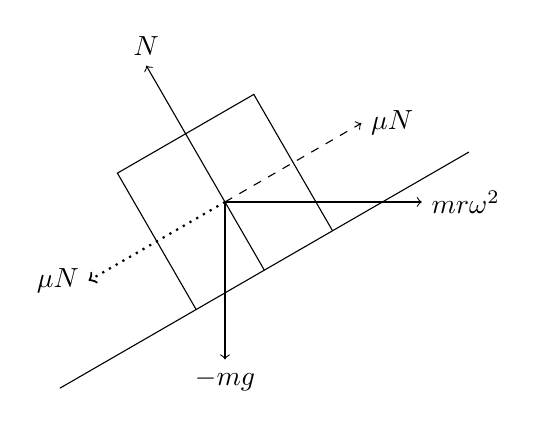
\begin{tikzpicture}
            %\draw[lightgray] (0, 0) grid (6, 6);
            \begin{scope}[rotate=30]
                \draw (0, 0) -- (6, 0);
                \draw (2, 0) -- (2, 2) -- (4, 2) -- (4, 0);
                \draw[->] (3, 0) -- (3, 3);
                \node[above] at (3, 3) {\(N\)};
                \draw[->, dashed] (3, 1) -- (5, 1);
                \draw[->, dotted, thick] (3, 1) -- (1, 1);
                \node[right] at (5, 1) {\(\mu N\)};
                \node[left] at (1, 1) {\(\mu N\)};
                \begin{scope}[rotate around={-30:(3, 1)}]
                    \draw[->] (3, 1) -- (5.5, 1);
                    \draw[->] (3, 1) -- (3, -1);
                    \node[right] at (5.5, 1) {\(mr\omega^2\)};
                    \node[below] at (3, -1) {\(-mg\)};
                \end{scope}
            \end{scope}
        \end{tikzpicture}
        \caption{Car on a banked track with possible frictions}
        \label{fig:banked track}
    \end{figure}
    A car is travelling around a circular track banked at \(\varphi = \SI{30}{\SIUnitSymbolDegree}\) with a radius of \(r = \SI{300}{m}\).
    First we will consider the case of a smooth track.
    At what speed must the car drive to not slip?
    
    We ignore the dotted and dashed lines in figure \ref{fig:banked track} as there is no friction.
    Separating into vertical and horizontal components we get respectively:
    \[N\cos\varphi = mg \qquad N\sin\varphi = mr\omega^2 = \frac{mv^2}{r}\]
    Dividing the horizontal component by the vertical gives
    \[\tan\varphi = \frac{v^2}{rg} \implies v = \sqrt{rg\tan\varphi}\]
    This gives a speed of \(v = \SI{41}{m.s^{-1}}\).
    
    What if instead we have friction?
    Take the coefficient of static friction to be \(\mu = 0.4\).
    The friction can act in one of two directions, up the track or down.
    This is the dashed and dotted lines on figure \ref{fig:banked track} respectively.
    This gives two cases:
    \begin{itemize}
        \item At speeds less than \(\SI{41}{m.s^{-1}}\) the friction acts up the track to stop the car slipping down
        \item At speeds greater than \(\SI{41}{m.s^{-1}}\) the friction acts down the track to stop the car slipping up
    \end{itemize}
    In the case that the car is slower than \(\SI{41}{m.s^{-1}}\) we get vertical and horizontal components
    \[mg = N\cos\varphi + \mu N\sin\varphi \qquad \frac{mv^2}{r} = N\sin\varphi - \mu N\cos\varphi\]
    \[N = \frac{mg}{\cos\varphi + \mu\sin\varphi}\]
    \[\frac{mv^2}{r} = mg\frac{\sin\varphi - \mu\cos\varphi}{\cos\varphi + \mu \sin\varphi}\]
    \[v^2 = rg\frac{\tan\varphi - \mu}{1 - \mu\tan\varphi}\]
    This gives \(v = \SI{21}{m.s^{-1}}\).
    We will now consider the case where the car is going faster than \(\SI{41}{m.s^{-1}}\).
    Now we get vertical and horizontal components
    \[mg = N\cos\varphi - \mu N \sin\varphi\qquad \frac{mv^2}{r} = N\sin\varphi + \mu N\cos\varphi\]
    \[N = \frac{mg}{\cos\varphi - \mu \sin\varphi}\]
    \[\frac{mv^2}{r} = mg\frac{\sin\varphi + \mu\cos\varphi}{\cos\varphi - \mu\sin\varphi}\]
    \[v^2 = rg\frac{\tan\varphi + \mu}{1 - \mu\tan\varphi}\]
    This gives \(v = \SI{61}{m.s^{-1}}\).
    This means that with friction any speed in the range \(\SI{21}{m.s^{-1}}\) to \(\SI{61}{m.s^{-1}}\) will result in no slipping.
    
    \example
    A charge \(q\) moving with velocity \(v\) in a magnetic field \(\vv B\) feels a Lorentz force
    \[\vv F = q\vv v\times \vv B\]
    This will give rise to circular motion, if the magnetic field is purely along the \(z\) axis then
    \[mr\omega^2 = qvB_z = q\omega rB_z \implies \omega = \frac{qB_z}{m}\]
    This is known as the cyclotron frequency.
    If there is also an electric field \(\vv E\) then the force is instead
    \[\vv F = q\vv E + q\vv v\times\vv B\]
    We will consider two cases:
    \begin{itemize}
        \item \(\vv E\) parallel to \(\vv B\). The magnetic field causes circular motion and the electric field causes linear acceleration.
        The result is that the charge corkscrews around the vector \(\vv B\) in the general direction of \(\vv B\).
        \item \(\vv E\) is perpendicular to \(\vv B\). The magnetic field causes circular motion and the electric field causes linear acceleration.
        The result is that the charge travels in the \(\vv E\) direction while in a spiral in the plane with normal \(\vv B\) following a cycloidal path.
    \end{itemize}
    In the latter case the force has components
    \begin{align*}
        F_x &= m\dv{v_x}{t} = qv_yB_z\\
        F_y &= m\dv{v_y}{t} = qv_xB_z + qE_y
    \end{align*}
    These are coupled equations as \(\dot v_x\) depends on \(v_y\) and \(\dot v_y\) depends on \(v_x\).
    
    \section{First order ODEs}
    \subsection{Fictitious Forces}
    When solving a problem in a non-inertial frame one can add a ``fictitious force" to pretend it is an inertial frame.
    For example going around a bend we add a centrifugal force outwards that accounts for the fact that our frame is non-inertial.
    
    \subsection{General Dynamics Approach}
    The general approach for a lot of dynamics problems is
    \begin{enumerate}
        \item Draw a diagram labelling all relevant quantities
        \item Choose a method (N2, conservation of energy, Lagrangian mechanics) to solve the problem and write down the equations
        \item Solve the (system of) ODEs
        \item Use boundary conditions/initial conditions to get constants of integration
        \item Obtain \(\vv x(t)\) and/or \(\vv v(t)\)
        \item Perform a sanity check (Consider: dimensions, limiting cases eg. \(t\to\infty\), \(m\to 0\), specific angles such that forces align, qualitative behaviour, does it match your intuition?)
    \end{enumerate}
    
    \subsection{ODEs}
    There will be a lot of differential equations in dynamics and physics in general.
    For this reason we will focus on solving them in general in this section and at other times throughout the course without worrying about where they come from.
    
    An ordinary differential equation (ODE) is a function \(f\) satisfying
    \[f(y(t), \dv{y}{t}, \dv[2]{y}{t},\dotsc ,\dv[n]{y}{t}, t) = 0\]
    The order of the differential equation is \(n\).
    A homogeneous ODE has no explicit dependence on \(t\) for example the following is a first order homogeneous ODE and the equation after is inhomogeneous:
    \[\dv{y}{t} + P(t)y = 0\]
    \[\dv{y}{t} + P(t)y = Q(t)\]
    A linear ODE only has \(y\) and its derivatives appear to the power of 1.
    For example the following don't occur in a linear ODE:
    \[y^-1,\qquad \left(\dv{y}{t}\right)^{1/2},\qquad \left(\dv[2]{y}{t}\right)^3\]
    Note that homogeneous and linear ODEs may not seem to be at first but they are if they can be rearranged into a homogeneous or linear ODE.
    
    Partial differential equations (PDEs) occur when instead \(y = y(t_1, \dotsc, t_n)\) and hence the differential equation contains partial derivatives of \(y\) or total derivatives since these can be written in terms of partial derivatives.
    
    \subsubsection{Separation of Variables}
    An ODE of the form
    \[\dv{y}{t} = f(t)g(y)\]
    can be written as
    \[\frac{1}{g(y)}\dv{y}{t} = f(t)\]
    Next we integrate both sides with respect to \(t\) to get
    \[\int \frac{1}{g(y)}\dv{y}{t}\,dt = \int f(t)\,dt\]
    The integral on the right hand side can then be found assuming sufficiently nice \(f\).
    We can use the fact that \(y = y(t)\):
    \begin{align*}
        y &= y(t)\\
        \dv{y}{t} &= \dv{y(t)}{t}\\
        dy &= \dv{y}{t}dt\\
    \end{align*}
    The term on the right hand side appears appears in the left hand side integral above:
    \[\int \frac{1}{g(y)}\dv{y}{t}\,dt = \int \frac{1}{g(y)}\,dy\]
    This integral can then be found assuming sufficiently nice \(1/g(y)\).
    
    \example
    Radioactive decay is described by the equation
    \[\dv{N(t)}{t} = -\lambda N(t)\]
    and the initial condition that \(N(0) = N_0\).
    Hence we can solve by separating variables:
    \[\frac{1}{N}\dv{N}{t} = -\lambda\]
    \[\int\frac{1}{N}\dv{N}{t}\,dt = -\lambda\int dt\]
    \[\int\frac{1}{N}\,dN = -\lambda t\]
    \[\ln N = -\lambda t + \ln C\]
    \[N = Ce^{-\lambda t}\]
    \[N(0) = N_0 = C\]
    \[N = N_0e^{-\lambda t}\]
    here we have used the trick of choosing a form for the constant of integration such that it simplifies later.
    This isn't necessary as we could always just rename the constant later to another constant but it can make it easier to think about.
    
    \example
    Generalised drag depends on both \(v\) and \(v^2\).
    The equation of motions for an object undergoing generalised drag can be written as
    \[\dv{v}{t} = av - bv^2\]
    \[\int\frac{1}{av - bv^2}\,dv = \int\, dt\]
    \[\frac{1}{av - bv^2} = \frac{1}{a}\left[\frac{1}{v} + \frac{b}{a - bv}\right]\]
    \[\frac{1}{a}\int\frac{1}{v} + \frac{b}{a - bv}\,dv = t\]
    \[\frac{1}{a}[\ln v - \ln(a - bv)] = t + \frac{\ln C}{a}\]
    \[\ln\left(\frac{v}{a - bv}\right) = at - \ln C\]
    \[\ln\left(\frac{a - bv}{v}\right) = - at + \ln C\]
    \[Ce^{-at} = \frac{a - bv}{v}\]
    We take the initial conditions to be \(v(0) = ak/b\) for some constant \(k\)
    \[v = \frac{a}{b}\left[\frac{1}{1 + (k - 1)e^{-at}}\right]\]
    When \(k = 1\) \(v = a/b\).
    
    \subsubsection{Substitution}
    It may be possible to choose a substitution such that separation of variables is possible.
    If we have
    \[\dv{y}{t} = f(y, t)\]
    then we choose \(u(y, t)\) for our substitution:
    \[\dv{u}{t} = \dv{u}{y}\dv{y}{t} = \dv{u}{y}f(y, t)\]
    We try to choose \(u\) such that the right hand side of this is separable, ie
    \[\dv{u}{y}f(y, t) = g(t)h(u)\]
    and this is solvable.
    This then allows us to find \(y\).
    
    \example
    \[\dv{y}{t} = f\left(\frac{y}{t}\right)\]
    Try \(u = y/t\), \(y = ut\):
    A more concrete example is
    \[\dv{y}{t} = \frac{y^2 + 2yt}{t^2} = \left(\frac{y}{t}\right)^2 + 2\left(\frac{y}{t}\right)\]
    choose \(y = ut\)
    \[\dv{y}{t} = u^2 + 2u\]
    \[\dv{y}{t} = \dv{t}[ut] = \dv{u}{t}t + u\dv{t}{t} = \dv{u}{t}t + u\]
    \[\dv{u}{t}t + u = u^2 + 2u\]
    \[\dv{u}{t}\frac{1}{u^2 + u} = \frac{1}{t}\]
    \[\int\frac{1}{u^2 + u}\,du = \int \frac{1}{t}\,dt\]
    \[\ln u - \ln(1 + u) = \ln t + \ln C\]
    \[y = \frac{Ct^2}{1 - Ct}\]
    
    \example
    \[\dv{y}{t} = f(at + by + c)\]
    Try \(u = at + by + c\)
    \[\dv{u}{t} = a + b\dv{y}{t} = a + bf(u)\]
    \[\frac{du}{a + bf(u)} = dt\]
    This can then be solved
    
    In general if
    \[\dv{y}{t} = f(g(y, t))\]
    then a good substitution to try is \(u = g(y, t)\).
    
    \subsubsection{Integrating Factors}
    This method will allow us to solve \emph{any} first order linear ODE.
    The most general form of one of these is
    \[\dv{y}{t} + P(t)y = Q(t)\]
    We now multiply through by some as yet unknown function \(\mu\):
    \[\mu(t)\left[\dv{y}{t} + P(t)y\right] = Q(t)\mu(t)\]
    We choose \(\mu\) such that
    \[\mu(t)Q(t) = \dv{t}[\mu(t)y] = \dv{\mu}{t}y + \mu\dv{y}{t}\]
    \[\mu\dv{y}{t} + P(t)\mu y = y\dv{\mu}{t} + \mu\dv{y}{t}\]
    \[P(t)\mu y = y\dv{\mu}{t}\]
    \[P(t)\mu = \dv{\mu}{t}\]
    \[\frac{1}{\mu}\dv{\mu}{t} = P(t)\]
    \[\int\frac{1}{\mu}\,d\mu = \int P(t)\, dt\]
    \[\ln\mu = \int P(t)\, dt + \ln C\]
    \[\mu = C\exp\left(\int P(t)\, dt\right)\]
    Since we multiply both sides of the original equation by \(\mu\) the \(C\)s cancel out and so we can choose any value we like.
    For simplicity we choose \(C = 1\).
    \[\mu(t) = \exp\left(\int P(t)\, dt\right)\]
    We had previously that
    \[Q(t)\mu(t) = \dv{t}[\mu(t)y]\]
    integrating both sides with respect to \(t\) gives us
    \[\int Q(t)\mu(t)\,dt + C = \mu(t)y\]
    where \(C\) is the constant of integration of \(\int Q\mu\,dt\).
    This allows us to say that
    \[y = \frac{1}{\mu(t)}\left[\int Q(t)\mu(t)\, dt + D\right]\]
    It is important to divide the constant of integration by \(\mu\) as well as the antiderivative.
    
    \example
    \[\dv{y}{t} + 2yt = 4t\]
    We identify \(P(t) = 2t\) and \(Q(t) = 4t\).
    \[\ln\mu = \int 2t\,dt = t^2 \implies \mu = e^{t^2}\]
    \[y = e^{-t^2}\left[\int 4te^{t^2}\,dt + C\right]\]
    \[= e^{-t^2}\left(2e^{t^2} + C\right)\]
    \[= 2 + Ce^{-t^2}\]
    
    \section{Bernoulli's Equation and Variable Mass}
    \subsection{Bernoulli's Equation}
    Bernoulli's equation is any differential equation that can be written in the form
    \[\dv{y}{t} + P(t)y = Q(t)y^n\]
    This is in general non-linear.
    In the cases that \(n = 0\) or \(n = 1\) this reduces to a form that can be solved by a method previously discussed.
    If this isn't the case then we have to make use of a specific substitution:
    \[u = y^{1-n}\]
    This gives us
    \[\dv{u}{t} = (1 - n)y^{-n}\dv{y}{t}\]
    \[\dv{y}{t} = \frac{y^n}{1-n}\dv{u}{t}\]
    Using \(y = y^nu\) we get
    \[\frac{y^n}{1 - n}\dv{u}{t} + P(t)y^nu = Q(t)y^n\]
    Cancelling the factors of \(y^n\) (assuming that \(y = 0\) the trivial solution is not the case)
    \[\frac{1}{1 - n}\dv{u}{t} + P(t)u = Q(t)\]
    This has now been reduced to a linear first order ODE which we can solve.
    
    \example
    \(n = 2\), \(u = 1/y\):
    \[\dv{y}{t} + P(t)y = Q(t)y^2\]
    \[-\dv{u}{t} + P(t)u = Q(t)\]
    \(n = 0.5\), \(u = \sqrt{y}\):
    \[\dv{y}{t} + P(t)y = Q(t)y^{1/2}\]
    \[2\dv{u}{t} + P(t)u = Q(t)\]
    
    \subsection{Logistic Equation}
    The logistic equation is used in modelling population growth.
    The size of the population is \(N\), the reproduction rate is \(r\) and there is some limited resource \(k\) that has to be shared between the entire population.
    The equation is
    \[\dv{N}{t} = rN\left(1 - \frac{N}{k}\right) = rN - \frac{r}{k}N^2\]
    \[\dv{N}{t} - rN = -\frac{r}{k}N^2\]
    This is Bernoulli's equation with \(n = 2\) so we can write it as
    \[\dv{u}{t} + ru = \frac{r}{k}\]
    where \(u = 1/N\).
    \[\int\frac{k}{1-ku}\,du = r\int dt\]
    \[-ln(1 - ku) = rt - \ln C\]
    \[u(t) = \frac{1}{k} + Ce^{-t}\]
    We have the initial condition that \(N(t=0) = N_0\) and hence \(u(t=0) = 1/N_0\).
    This means that the constant is
    \[C = \frac{1}{N_0} - \frac{1}{k}\]
    Rewriting in terms of \(N\) and rearranging we get
    \[N(t) = \frac{kN_0}{N_0\left(1 - e^{-rt}\right) + ke^{-rt}}\]
    This gives a curve that increases rapidly from \(N_0\) before flattening off and asymptoting a value of \(k\).
    
    \subsection{Variable Mass}
    Up until now we have only considered constant mass problems but there are many situations where the mass of an object is not constant.
    This means that either there must be a force or there must be a change in velocity to cancel out the effect of the mass change in Newton's second law:
    \[\vv F = \dv{\vv p}{t} = m\dv{\vv v}{t} + \dv{m}{t}\vv v\]
    
    \example
    A train has initial mass \(M_0\) and velocity \(v_0\).
    It is raining and the train is collecting water at a rate \(\mu\).
    Find the equation for the velocity of the train at a time \(t\).
    Assume that the rain falls vertically.
    
    The mass of the train as a function of time is
    \[M(t) = M_0 + \mu t\]
    The force in the \(x\) direction is \(F_x = 0\).
    This means that we can write Newton's second law in the \(x\) direction as
    \[\dv{v}{t} = -\frac{v}{M}\dv{M}{t} = -\frac{v\mu}{M_0 + \mu t}\]
    \[\int\frac{1}{v}\,dv = -\int\frac{\mu}{M_0 + \mu t}\,dt\]
    \[\ln v = -\ln(M_0 + \mu t) + \ln C\]
    \[v = \frac{M_0v_0}{M_0 + \mu t}\]
    We can also solve this same problem much faster with Newton's third law:
    
    Initially \(p = M_0v_0\).
    After a time \(t\) the momentum is \(p = Mv = (M_0 + \mu t)v\).
    Equating these we get
    \[M_0v_0 = (M_0 + \mu t)v\]
    \[v = \frac{M_0v_0}{M_0 + \mu t}\]
    Note that as \(t\to \infty\) \(v\propto 1/t\).
    
    \example
    The same train now has a drain installed in the bottom that is sufficiently large that the flow of water out can keep up with the flow of water in.
    After some time the train then has mass \(M(t) = M\) since no rain stays on the train so the mass doesn't increase.
    At time \(t\) the velocity is \(v\).
    At time \(t + dt\) the velocity is \(v + dv\).
    During the time interval \(dt\) a mass of \(\mu dt\) water drains out of the train.
    The momentum loss due to this is \(\mu dt v\).
    Initially the momentum of the train is \(p = Mv\).
    At time \(t + dt\) the momentum of the train is \(p = M(v + dv) + \mu vdt\)
    Equating we get
    \[Mv = Mv + Mdv + \mu vdt\]
    \[0 = Mdv + \mu vdt\]
    \[M\int\frac{1}{v}\,dv = -\mu\int dt\]
    \[v = v_0e^{-\mu t/M}\]
    As \(t\to\infty\) \(v\propto e^{-kt}\).
    This decreases much faster than \(1/t\) which is how the velocity of the train that keeps the water changes.
    This is counter-instinctual at first but we need to consider the momentum lost to the water that drains out of the train as well as the loss of velocity caused by the gain of mass.
    
    \section{Variable Mass and Energy}
    \example
    A raindrop gains mass as it falls.
    The first (somewhat unrealistic) model we will use is that the rate of mass accretion is proportional to the mass:
    \[\dv{m}{t} \propto m \implies \dv{m}{t} = \alpha m\]
    For some constant \(\alpha\).
    We can find the mass as a function of time:
    \[\int \frac{1}{m}\,dm = \alpha\int dt\]
    \[\ln m = \alpha t + \ln C\]
    \[m = Ce^{\alpha t}\]
    \[m(t) = m_0e^{\alpha t}\]
    where we have used the condition \(m(t=0) = m_0\).
    We can apply Newton's second law an we get
    \[-mg = m\dv{v_z}{t} + v_z\dv{m}{t}\]
    \[-mg = m\dv{v_z}{t} + v_z\alpha m\]
    \[-g = \dv{v_z}{t} + \alpha v_z\]
    \[\dv{v_z}{t} = -g - \alpha v_z\]
    \[\int\frac{1}{-g - \alpha v_z}\,dv_z = \int dt\]
    \[-\frac{1}{\alpha}\ln(-g-\alpha v_z) = t - \frac{\ln C}{\alpha}\]
    \[\ln(-g - \alpha v_z) = -\alpha t + \ln C\]
    \[-g - \alpha v_z = Ce^{-\alpha t}\]
    Apply the initial condition that \(v_z(t = 0) = 0\)
    \[-g = C\]
    \[-g - \alpha v_z = -ge^{-\alpha t}\]
    \[v_z = -\frac{g}{\alpha}\left(1 - e^{-\alpha t}\right)\]
    As \(t\to \infty\) we get
    \[v_z \to -\frac{g}{\alpha}\]
    The second model we consider is that mass is accrued at a constant rate.
    \[\dv{m}{t} = k\]
    This gives us mass as a function of time:
    \[m(t) = kt + m_0\]
    where again \(m(t = 0) = m_0\).
    Applying Newton's second law:
    \[-mg = m\dv{v_z}{t} + v_z\dv{m}{t}\]
    \[-mg = m\dv{v_z}{t} + kv_z\]
    \[\dv{v_z}{t} = -g - \frac{kv_z}{kt + m_0}\]
    where we have chosen to write mass as a function of time.
    \[\dv{v_z}{t} + \frac{k}{kt + m_0}v_z = -g\]
    \[P(t) = \frac{k}{kt + m_0},\qquad Q(t) = -g,\qquad \mu(t) = \exp\left(\int \frac{k}{kt + m_0} \,dt\right) = \exp(\ln(kt + m_0)) = kt + m_0\]
    \[v_z = \frac{1}{kt + m_0}\left[\int -g(kt + m_0)\,dt + C\right]\]
    \[v_z = -\frac{g}{kt + m_0}\left[\frac{kt^2}{2} + m_0t - \frac{C}{g}\right]\]
    Applying the initial condition that \(v_z(t=0) = 0\):
    \[0 = \frac{C}{m_0}\implies C = 0\]
    \[v_z = -\frac{gt}{kt + m_0}\left[\frac{kt}{2} + m_0\right]\]
    As \(t\to \infty\) we get
    \[v_z\to -\frac{1}{2}gt\]
    which, unlike the previous case, is not constant.
    This value is exactly half of what we would get for a particle in free fall with no mass accretion.
    The reason it is lower is that velocity has to be lost to account for the increase in mass.
    Since the rate of accretion is constant at some point it becomes negligible compared to the size of the raindrop.
    
    \subsection{The Rocket Equation}
    Consider a rocket of mass \(M_0\) that is carrying fuel of mass \(m_0\) which it will burn.
    The mass of fuel burnt as a function of time is \(m(t)\).
    The total mass of the rocket is as a function of time is then
    \[M(t) = M_0 - m(t)\]
    The exhaust velocity of the rocket is \(u\) relative to the speed of the rocket.
    In time \(dt\) the rocket loses a momentum of \(udm\) due to loss of mass at a velocity.
    The momentum gain due to increased velocity of the rocket from speed \(v\to v + dv\) is \(Mdv\).
    Differentiating \(M(t)\) with respect to time we get
    \[\dv{M}{t} = -\dv{m}{t} \implies dM = -dm\]
    Equating the two momentum changes since they must cancel to no change in overall momentum an using the fact that \(dM = -dm\) we get
    \[Mdv = -udm = -udM\]
    \[\int dv = -u\int\frac{1}{M}\,dM\]
    \[v(M) = -u\ln M + u\ln C\]
    \[v(t) = -u\ln(M(t)) + u\ln C\]
    \[v(t) = u\ln\left(\frac{C}{M(t)}\right)\]
    Applying the initial condition \(M(t=0) = M_0 + m_0\) and \(v(t=0) = 0\) we get
    \[0 = u\ln\left(\frac{C}{M_0 + m_0}\right)\implies C = M_0 + m_0\]
    \[v(t) = u\ln\left(\frac{M_0 + m_0}{M(t)}\right)\]
    At the time \(T\) all of the fuel has been burned, this means \(M(T) = M_0\).
    \[v(T) = u\ln\left(\frac{M_0 + m_0}{M_0}\right) = u\ln\left(1 + \frac{m_0}{M_0}\right)\]
    The right hand side is independent of time so any way that you burn the fuel the final velocity will be the same for the same values of \(M_0\) and \(m_0\).
    \(u\) doesn't need to be greater than the escape velocity which is good since that would be impractical and maybe impossible without destroying the rocket.
    To make a rocket as fast as possible it is desirable to have \(u\) be as large as possible and to have \(m_0/M_0\) be as large as possible so you want a lot of fuel compared to the mass of the rocket.
    Escape velocity is about \(\SI{12}{km.s^{-1}}\) and typical values of \(u\) are about \(\SI{2}{km.s^{-1}}\).
    In this case it is necessary to have \(m_0/M_0\approx400\) this is obviously quite difficult to do.
    
    If we want to include the effects of gravity then the problem becomes more complex.
    We assume that the fuel burn happens close enough to the ground that the gravitational field strength can be approximated as constant during the burn.
    We can write Newton's second law as
    \[M\dv{v}{t} + v\dv{M}{t} = -Mg\]
    \[\int\, dv = -u\int\frac{1}{M}\,dM - g\int\,dt\]
    \[v(t) = u\ln\left(\frac{M_0 + m_0}{M(t)}\right) - gt\]
    Here the right hand side does depend on \(t\).
    To achieve the highest possible velocity we want to burn the fuel as quickly as possible to counteract this.
    
    \subsection{Conservation of Energy}
    \subsubsection{Definitions}
    If a particle moves from point \(A\) to point \(B\) starting at time \(t_A\) and ending at time \(t_B\) then we define the impulse as the change in momentum:
    \[\text{impulse} = \Delta\vv p = \vv{p_B} - \vv{p_A} = \int_{t_A}^{t_B}\dv{\vv p}{t}\,dt = \int_{t_A}^{t_B}\vv F\,dt\]
    where we have Newton's second law to write this in terms of the force \(\vv F\) that causes the change in momentum.
    If the path taken is composed of path elements \(d\vv l\) then we define the work done to travel along the path as
    \[W = \int_{t_A}^{t_B}\vv F\cdot d\vv l\]
    The path is necessarily parallel to the velocity so \(d\vv l = \vv vdt\) which gives
    \[W = \int_{t_A}^{t_B}\vv F\cdot\vv v\,dt = \int_{t_A}^{t_B}P\,dt\]
    where we define \(\vv F\cdot\vv v = P\) as the power.
    Assuming constant mass we can use Newton's second law to write this as
    \[W = \int_{t_A}^{t_B} m\dv{\vv v}{t}\cdot\vv v\, dt = \int_{t_A}^{t_B}\vv v\cdot d\vv v = \left[\frac{1}{2}mv^2\right]_{t_A}^{t_B}\]
    We define the (non-relativistic) kinetic energy, \(T\), as
    \[T = \frac{1}{2}mv^2\]
    From this definition we get that work done is the change in kinetic energy:
    \[W = \Delta T = T_B - T_A\]
    We define the scalar potential for a force \(\vv F\) as the scalar field \(V\) such that 
    \[\vv F = -\grad V(\vv r)\]
    For example the gravitational potential is
    \[V(\vv r) = -\frac{GMm}{r}\implies \vv F = -\grad V = GMm\grad\frac{1}{r} = -\frac{GMm}{r^2}\vh r\]
    This works for any conservative force \(\vv F\).
    It is often easier to solve problems with potentials since it is a scalar quantity and then we can find the gradient if we need the force.
    If the scalar potential is graphed, since the negative of the gradient points in the direction of steepest descent, we can think about the force causing a ball at a point to roll down the potential.
    This gives a good intuitive way of thinking about the relation between potential and force and is the reason that the negative gradient was chosen rather than the positive gradient.
    
    \part[Simple Harmonic Motion]{Simple Harmonic Motion\\[\bigskipamount]\large SHM, Second Order ODEs, Damping, Forced Oscillations, Resonance, Coupled Oscillations}
    \section{Conservative Forces and SHM}
    \subsection{Conservative Forces}
    A conservative force \(\vv F\) causes an object to move from point \(A\) to point \(B\) and have a change in potential of \(\Delta V = V_B - V_A\).
    The work done is
    \[W = \int_A^B\vv F\cdot d\vv l = -\int_A^B\grad V\cdot d\vv l\]
    \[d\vv l = dx_i\ve i\]
    \[\grad V = \ve i\pdvx i V\]
    \[\grad V\cdot d\vv l = \pdv{V}{x_i}dx_i = dV\]
    \begin{align*}
        W &= -\int_A^B dV\\
        &= -(V_B - V_A)\\
        &= -\Delta V
    \end{align*}
    If the force can be written as \(-\grad V\) then the force is conservative since \(W_{AB} = -\Delta V\) and \(W_{BA} = \Delta V\) so \(W_{AA} = -\Delta V + \Delta V = 0\) so no work is done around a close loop.
    The following are conditions for a force to be conservative:
    \begin{itemize}
        \item The force depends only on position.
        This means that force can be written \(\vv F = \grad V(\vv r)\) which is only dependent on position.
        \item The path integral of \(\vv F\) around a closed loop is zero.
        \[\oint \vv F\cdot d\vv l = 0\]
        \item The force is irrotational.
        That is it has zero curl.
        This can be seen from the fact that the curl of a gradient is zero.
        \[\curl\grad V = \vv 0 \implies -\curl\vv F = \vv 0\]
    \end{itemize}
    Using Stoke's Theorem:
    \[\int_S (\curl\vv a)\cdot d\vv S = \oint_C \vv a\cdot d\vv r\]
    we can show that the last two conditions are equivalent:
    \[\oint \vv F\cdot d\vv l = \int (\curl\vv F)\cdot d\vv S = 0\]
    we know by the first of the two conditions that this must be equal to zero and for this to be true for arbitrary \(S\) the curl must be zero.
    
    A conservative force conserves energy.
    The work done is \(W = \Delta T\), that is the change in kinetic energy.
    Also we have shown that \(W = -\Delta V\).
    Equating and rearranging we get
    \[\Delta T + \Delta V = 0\]
    We define the energy as a value
    \[E = T + V\]
    which is constant for conservative forces.
    This same quantity is defined as the Hamiltonian \(\mathcal H\) for a conservative force in Hamiltonian mechanics.
    
    \example
    What is the escape velocity of Earth?
    Define the escape velocity as \(v_0\).
    The initial kinetic energy of an object at this velocity is \(T_i = mv_0^2/2\).
    The potential energy of this object initially is
    \[V_i = -\frac{GMm}{R_E}\]
    To escape the potential well of Earth's gravity we need to go to infinity where \(V_f = 0\) and we want the minimum velocity to do this such that we just run out of kinetic energy at this point so \(T_f = 0\).
    Since the energy between these two points must be conserved we get
    \[T_i + V_i = T_f + V_f = 0 + 0 = 0\]
    \[\frac{1}{2}mv_0^2 = \frac{GMm}{R_E}\]
    \[v_0 = \sqrt{\frac{2GM}{R_E}} = \SI{11.8}{km.s^{-1}}\]
    Note that this is independent of direction so if you could run at \(\SI{11.8}{km.s^{-1}}\) assuming no dissipative forces you would be able to escape Earth.
    
    \subsection{Simple Harmonic Oscillators}
    We define equilibrium as \(\vv F = \vv 0\) so \(-\grad V = 0\).
    In one dimension at equilibrium we have
    \[\dv{V}{x} = 0\]
    We define \(x = 0\) to be at the equilibrium position.
    We can Taylor expand the potential to get
    \[V(x) = V(0) + x\dvat{V}{x}{x=0} + \frac{1}{2}x^2\dvat[2]{V}{x}{x=0} + \mathcal O(x^3)\]
    From the definition of equilibrium the second term must be zero.
    We can define \(V = 0\) anywhere we like so we define \(V(0) = 0\).
    This leaves us, for sufficiently small \(x\), with
    \[V(x) = \frac{1}{2}x^2\dvat[2]{V}{x}{x=0} = \frac{1}{2}kx^2\]
    \[k = \dvat[2]{V}{x}{x=0}\]
    This gives a force of
    \[F = -\dv{V}{x} = -kx\]
    This is Hooke's law for a spring.
    Using Newton's second law we get
    \[m\dv[2]{x}{t} = -kx\]
    We define \(\omega_0\), the natural frequency, as
    \[\omega_0 = \sqrt{\frac{k}{m}}\]
    allowing us to write the equation of motion as
    \[\dv[2]{x}{t} + \omega_0^2x = 0\]
    We make the ansatz:
    \[x = e^{\lambda t}\implies \dv[2]{x}{t} = \lambda^2e^{\lambda t} = \lambda^2 x\]
    \[\lambda^2 x + \omega_0^2 x = 0\]
    \[\lambda^2 = -\omega_0^2\]
    \[\lambda = \pm i\omega_0\]
    
    There are three equivalent solutions to this equation.
    They are
    \begin{itemize}
        \item Exponential form:
        \[x(t) = C_1e^{i\omega_0 t} + C_2e^{-i\omega_0 t}\]
        \item Sine/cosine form:
        \[x(t) = A_1\sin(\omega_0 t) + A_2\cos(\omega_0 t)\]
        \item Amplitude/phase form:
        \[x(t) = A\sin(\omega_0t + \delta) = A\cos(\omega_0t + \delta')\]
    \end{itemize}
    The constants are related by the following:
    \[A_1 = iC_1 - iC_2,\qquad A_2 = C_1 + C_2\]
    \[A = \sqrt{A_1^2 + A_2^2},\qquad \delta = \arctan\left(\frac{A_2}{A_1}\right)\]
    \[\delta' = \delta - \frac{\pi}{2},\qquad A = 2\sqrt{C_1C_2}\]
    The form that you use depends on what you are trying to do.
    For example it is easier to solve in terms of exponentials but the amplitude/phase form gives more information about what is happening physically.
    
    \section{SHM, Period and Damping}
    \subsection{Pendulum}\label{sec:pendulum}
    A pendulum bob is hung from a light rod, length \(L\), and allowed to swing freely as shown in figure \ref{fig:pendulum}
    \begin{figure}[ht]
        \centering
        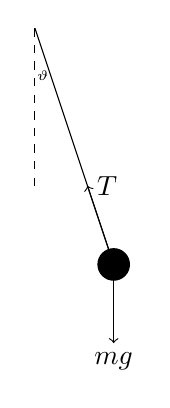
\begin{tikzpicture}
            \draw (0, 4) -- (1, 1);
            \draw[fill=black] (1, 1) circle (0.2);
            \draw[->] (1, 1) -- (1, 0);
            \node[below] at (1, 0) {\(m\vv g\)};
            \draw[dashed] (0, 4) -- (0, 2);
            \node at (0.1, 3.4) {\tiny\(\vartheta\)};
            \draw[->] (1, 1) -- (0.6667, 2);
            \node[right] at (0.6667, 2) {\(\vv T\)};
        \end{tikzpicture}
        \caption{Pendulum force diagram}
        \label{fig:pendulum}
    \end{figure}
    Due to the circular symmetry of the situation it is best to work in polar coordinates.
    This means that the position and its time derivatives are
    \[\vv r = L\vh r\]
    \[\vv v = \dv{\vv r}{t} = L\dv{\vh r}{t} = L\dv{\vartheta}{t}\vh\vartheta\]
    \[\vv a = \dv{\vv v}{t} = L\dv{t}\left[\dv{\vartheta}{t}\vh\vartheta\right] = L\dv[2]{\vartheta}{t}\vh\vartheta + L\dv{\vartheta}{t}\dv{\vh\vartheta}{t} = L\dv[2]{\vartheta}{t}\vh\vartheta - L\left(\dv{\vartheta}{t}\right)^2\vh r\]
    Where we have used the derivatives of the unit vectors derived in section \ref{sec:polar unit vector derivatives}:
    \[\dv{\vh r}{\vartheta} = \vh\vartheta\]
    \[\dv{\vh\vartheta}{\vartheta} = -\vh r\]
    We can decompose the forces into these unit vectors:
    \[\vv T = -T\vh r\]
    \[m\vv g = mg\cos\vartheta\vh r - mg\sin\vartheta\vh\vartheta\]
    Using Newton's second law this gives us
    \[mL\dv[2]{\vartheta}{t} = -mg\sin\vartheta\]
    \[-mL\left(\dv{\vartheta}{t}\right)^2 = mg\cos\vartheta - T\]
    From the first of these two equations if we assume \(\vartheta\) is small and cancel the masses we get
    \[\dv[2]{\vartheta}{t} = -\frac{g}{L}\vartheta\]
    We define the natural frequency as
    \[\omega_0 = \frac{g}{L}\]
    which gives us
    \[\dv[2]{\vartheta}{t} = -\omega_0\vartheta\]
    This is simple harmonic motion at a frequency \(\omega_0\) and has a solution
    \[\vartheta = A_\vartheta\sin(\omega_0 t + \delta)\]
    The velocity is then
    \[v = L\dv{\vartheta}{t} = LA_\vartheta\omega_0\cos(\omega_0 t + \delta)\]
    Taking the second of the two Newton's second law equations we get
    \begin{align*}
        T &= mg\cos\vartheta + mL\left(\dv{\vartheta}{t}\right)^2\\
        &= mg\left(1 - \frac{\vartheta^2}{2}\right) + \frac{mv^2}{L}\\
        &= mg - \frac{1}{2}mg\vartheta^2 + \frac{mv^2}{L}
    \end{align*}
    \(T\) is minimised when \(\vartheta = A_\vartheta\) and \(v = 0\):
    \[T_\text{min} = mg\left(1 - \frac{1}{2}A_\vartheta^2\right)\]
    \(T\) is maximised when \(\vartheta = 0\) and the velocity is at a maximum:
    \[T_\text{max} = mg\left(1 + a_\vartheta^2\right)\]
    We can find the kinetic energy \(K\) and potential energy \(T\):
    \[K = \frac{1}{2}mv^2 = \frac{1}{2}mL^2\left(\dv{\vartheta}{t}\right)^2\]
    \[V = mgh = mg(L - L\cos\vartheta)\]
    
    \subsection{Energy Conservation}
    Both \(K\) and \(V\) depend on time but since \(E = K + T\) is conserved we know that
    \[\dv{E}{t} = \dv{t}[K + T] = 0\]
    \[\dv{K}{t} = \dv{t}\left[\frac{1}{2}mL^2 \left(\dv{\vartheta}{t}\right)^2\right] = mL^2\dv{\vartheta}{t}\dv[2]{\vartheta}{t}\]
    \[\dv{V}{t} = \dv{t}\left[mgL = mgL\cos\vartheta\right] = mgL\sin\vartheta\dv{\vartheta}{t}\]
    \[\dv{E}{t} = ml^2\dv{\vartheta}{t}\dv[2]{\vartheta}{t} + mgL\sin\vartheta\dv{\vartheta}{t} = 0\]
    \[L\dv[2]{\vartheta}{t} + g\sin\vartheta = 0\]
    This shows that sometimes it is possible to find the equations of motion from conservation of energy.
    
    \subsection{Period of Oscillation}
    \[v = \dv{x}{t}\]
    \[t = \int_{-A}^A\frac{1}{v}\,\dd x\]
    The period \(\tau = 2t\) is twice the time taken to go from \(-A\) to \(A\).
    We can write the velocity in terms of the kinetic energy as
    \[v = \sqrt{\frac{2K}{m}} = \sqrt{\frac{2(E - V)}{m}}\]
    \[K = \frac{1}{2}mA^2\omega_0^2\cos^2(\omega_0 t + \delta) = \frac{1}{2}kA^2\cos^2(\omega_0 t + \delta)\]
    \[V = \frac{1}{2}kx^2 = \frac{1}{2}kA^2\sin^2(\omega_0 t + \delta)\]
    \[E = K + T = \frac{1}{2}kA^2(\cos^2(\omega_0 t + \delta) + \sin^2(\omega_0 t + \delta))\]
    This gives us \(v\) as a function of \(x\), allowing us to do the integral
    \[\tau = 2\sqrt{2m}\int_{-A}^A\frac{1}{\sqrt{\frac{1}{2}kA^2 - \frac{1}{2}kx^2}}\,\dd x\]
    The solution to this integral can be found using \(x = A\sin u\) as a substitution.
    \[\dv{x}{u} = A\cos u \implies \dd x = A\cos u\dd u\]
    \[\tau = 2\sqrt{2m}\int_{-\pi/2}^{\pi/2}\frac{\cos u}{\sqrt{\frac{1}{2}kA^2 - \frac{1}{2}kA^2\sin^2u}}\,\dd u\]
    \[\tau = 2\sqrt{\frac{m}{k}}\int_{-\pi/2}^{\pi/2}\frac{\cos u}{\sqrt{
    1 - \sin^2 u}}\,\dd u = 2\sqrt{\frac{m}{k}}\int_{-\pi/2}^{\pi/2}\dd u\]
    \[\tau = 2\pi\sqrt{\frac{m}{k}}\]
    
    \subsection{Damping}
    We can add friction to the system which we assume is proportional to velocity.
    The resulting equation is
    \[F = m\dv[2]{x}{t} = -kx - b\dv{x}{t}\]
    We make the ansatz that \(x = e^{\lambda t}\) for some \(\lambda\in\bb C\). We also define \(\gamma = b/2m\) and \(\omega_0^2 = k/m\).
    Dividing through by \(m\) and substituting in these new definitions we get
    \[\dv[2]{x}{t} + 2\gamma\dv{x}{t} + \omega_0^2 x = 0\]
    We can substitute in the ansatz for \(x\) and we get
    \[\lambda^2e^{\lambda t} + 2\gamma\lambda e^{\lambda t} + \omega_0^2e^{\lambda t} = 0\]
    Since \(e^{\lambda t}\ne 0\A\lambda\) we can divide through by \(e^{\lambda t}\) to get
    \[\lambda^2 + 2\gamma\lambda + \omega_0^2 = 0\]
    \[\lambda = \frac{-2\gamma \pm \sqrt{4\gamma^2 - 4\omega_0^2}}{2} = -\gamma \pm \sqrt{\gamma^2 - \omega_0^2}\]
    Since there are two different values of \(\lambda\) there are two different solutions to the differential equation which is what we would expect since it is second order.
    The general solution is a linear combination of these two solutions.
    We define \(\omega = \sqrt{\omega_0^2 - \lambda^2}\).
    The general solution can then be written as
    \[x(t) = e^{-\gamma t}\left[C_1e^{i\omega t} + C_2e^{-i\omega t}\right]\]
    There are two terms here.
    The first is the \(e^{-\gamma t}\) term.
    This is the damping term and causes the oscillation to decay away.
    The rest can be identified as oscillations at some frequency \(\omega \ne \omega_0\).
    \section{Damped and Driven Oscillations}
    Exactly how the damped oscillations look depends on the size of \(\omega_0\) compared to \(\gamma\).
    If \(\omega _0 > \gamma\) then \(\omega\in\bb R\) so the oscillating term is still oscillatory and the damped term just reduces the amplitude each oscillation.
    This is under-damped simple harmonic motion.
    
    If \(\gamma > \omega_0\) then \(\omega = i\omega'\) for some \(\omega' = \bb R\).
    The \(i\) in this term cancels with the \(i\) in the oscillating term so this term stops being oscillatory and the amplitude just slowly decays to zero without oscillation.
    This is over-damped simple harmonic motion.
    
    If \(\gamma = \omega_0\) then \(\omega = 0\) the analysis that lead to an equation for \(x\) is flawed as we assumed two distinct \(\lambda\).
    In this case the actual solution is given by
    \[x(t) = (C_1 + C_2t)e^{-\gamma t}\]
    Again there is no oscillation.
    See section \ref{sec:d'Alambert's method} for where this equation comes from.
    
    \subsection{Second Order ODEs}
    A homogeneous second order ODE can be written as
    \[\dv[2]{y}{t} + P(t)\dv{y}{t} + Q(t)y = 0\]
    If \(P\) and \(Q\) are constant we can solve this as before.
    We make the ansatz that \(y = e^{\lambda t}\) and we get
    \[\lambda^2 + P\lambda + Q = 0\]
    after substitution and simplification.
    \[\lambda_1, \lambda_2 = \frac{-P \pm \sqrt{P^2 - 4Q}}{2}\]
    \[y(t) = C_1e^{\lambda_1 t} + C_2e^{\lambda_2 t}\]
    
    \subsection{D'Alambert's method}\label{sec:d'Alambert's method}
    If \(P\) and \(Q\) aren't constant then there is no general method that guarantees a solution.
    If we know one solution already (or can guess it) then we can use d'Alambert's method to find the other.
    Let \(y_1\) be the solution we know and \(y_2\) be the solution we seek.
    We know that both \(y_1\) and \(y_2\) must satisfy
    \[\dv[2]{y}{t} + P(t)\dv{y}{t} + Q(t)y = 0\]
    We define a new function \(u(t)\) such that \(y_2 = uy_1\).
    This gives the first and second derivatives of \(y_2\) as
    \[\dv{y_2}{t} = y_1\dv{u}{t} + u\dv{y_1}{t}\]
    \[\dv[2]{y_2}{t} = y_1\dv[2]{u}{t} + 2\dv{y_1}{t}\dv{u}{t} + u\dv[2]{y_1}{t}\]
    We can substitute this into the original differential equation:
    \[y_1\dv[2]{u}{t} + 2\dv{y_1}{t}\dv{u}{t} + u\dv[2]{y_1}{t} + Py_1\dv{u}{t} + Pu\dv{y_1}{t} + Quy_1 = 0\]
    Rearranging we get
    \[y_1\dv[2]{u}{t} + 2\dv{y_1}{t}\dv{u}{t} + u\left[\dv[2]{y_1}{t} + P\dv{y_1}{t} + Qy_1\right] + Py_1\dv{u}{t} = 0\]
    We can see that from the original differential equation the part in brackets is zero.
    \[y_1\dv[2]{u}{t} + 2\dv{y_1}{t}\dv{u}{t} + Py_1\dv{u}{t} = 0\]
    Since \(y_1\) is a known function this is first order in \(\dd u/\dd t\) and if we solve for \(u\) we can use this to find \(y_2\).
    
    \example
    \[t^2\dv[2]{y}{t} - 2t\dv{y}{t} + (2 - t^2)y = 0\]
    One solution to this is \(y_1(t) = te^{-t}\).
    We can identify that \(P(t) = -2/t\) as we have to divide through by \(t^2\) to get \(\dd^2 y/\dd t^2\)  on its own.
    By d'Alambert's method we know that
    \[te^{-t}\dv[2]{u}{t} - 2te^{-t}\dv{u}{t} = 0\]
    When \(t\ne 0\) we get
    \[\dv[2]{u}{t} - 2\dv{u}{t}\]
    which we can solve to get
    \[\dv{u}{t} = Ce^{2t}\]
    Integrating this gives us
    \[u = \frac{C}{2}e^{2t}\]
    From here we can get the second solution
    \[y_2 = uy_1 = \frac{C}{2}e^{2t}e^{-t} = \frac{C}{2}e^{t}\]
    
    If we consider the case we had for damped simple harmonic motion before where \(\gamma = \omega_0\) we had one solution \(y_1 = Ce^{-\gamma t}\).
    We can identify \(P(t) = 2\gamma\) and by d'Alambert's method we know that
    \[Ce^{-\gamma t}\dv[2]{u}{t} - 2\gamma C e^{-\gamma t}\dv{u}{t} + 2\gamma PCe^{-\gamma t}\dv{u}{t} = 0\]
    \[\dv[2]{u}{t} = 0\]
    \[\dv{u}{t} = D\]
    \[u = Dt + E\]
    \[y_2 = Dte^{-\gamma t} + Ee^{-\gamma t}\]
    the general solution is then
    \[y = ((C + E) + tD)e^{-\gamma}\]
    which is what we had before with \(C_1 = C + E\) and \(C_2 = D\).
    
    \subsection{Driven Oscillations}
    An inhomogeneous second order ODE can be written as
    \[\dv[2]{y}{t} + P(t)\dv{y}{t} + Q(T)y = F(t)\]
    In this case the solution has the form
    \[y = y_p + y_c\]
    where \(y_p\), known as the particular solution, depends on the form of \(F\) and \(y_c\), known as the complementary solution, is the solution to the equation if \(F(t) = 0\).
    The complementary solution is itself the linear combination of two solutions and can be found using the methods above.
    To find the particular solution we consider the form of \(F\) and pick a similar form to try as an ansatz and solve for constants.
    Some of the common forms are given in table \ref{tab:F and y_p}.
    In general the function chosen for \(y_p\) should be the most general function of a form similar to \(F\).
    \begin{table}[ht]
        \centering
        \begin{tabular}{c|c}\hline
            \(F(t)\) & \(y_p(t)\) \\\hline
            \(ae^{kt}\) & \(Ae^{kt - \delta)}\)\\
            \(a\sin kt\) & \(A\cos kt + B\sin kt\) or \(A\sin(kt + \delta)\)\\
            \(a_0 + a_1t + a_2 t+\dotsb+ a_nt^n\) & \(A_0 + A_1t + A_2 t+\dotsb+ A_nt^n\)\\\hline
        \end{tabular}
        \caption{Some common forms of \(F\) and the suggested forms of \(y_p\)}
        \label{tab:F and y_p}
    \end{table}

    \example
    Suppose \(F(t) = F_0e^{i\Omega t}\).
    We can apply Newton's second law and divide through by mass to get an equation of the form
    \[\dv[2]{x}{t} + 2\gamma\dv{x}{t} + \omega_0^2 = A_0e^{i\Omega t}\]
    where \(A_0 = F_0/m\).
    The complementary solution is found, as before, to be
    \[x_c = C_1e^{\lambda_1 t} + C_2e^{\lambda_2 t}\]
    where \(\lambda_{1},\lambda_2 = -\gamma\pm i\omega\) and \(\omega = \sqrt{\omega_0^2 - \gamma^2}\).
    We make the ansatz that
    \[x_p = Ae^{i(\Omega t - \delta)}\]
    We can substitute this into the differential equation to get
    \[A[-\Omega^2 + 2i\gamma\Omega + \omega_0^2]e^{i\Omega t}e^{-i\delta} = A_0e^{i\Omega t}\]
    \[(\omega_0^2 - \Omega^2)A + 2i\gamma\Omega A = A_0e^{i\delta} = A_0\cos\delta + iA_0\sin\delta\]
    Equating the real and imaginary parts we get
    \[(\omega_0^2 - \Omega^2)A = A_0\cos\delta\]
    \[2\gamma\Omega A = A_0\sin\delta\]
    Dividing the imaginary part by the real part
    \[\tan\delta = \frac{2\gamma\Omega}{\omega_0^2 - \Omega}\]
    Solving the real and imaginary parts for \(A\) instead we get
    \[A = \frac{A_0}{\sqrt{(\omega_0^2 - \Omega^2)^2 + (2\gamma\Omega)^2}}\]
    
    \section{Properties of Forced Oscillations}
    The general solution to a damped, driven, simple harmonic oscillator is
    \[x(t) = x_c(t) + x_p(t)\]
    If there is any damping then as \(t\to\infty\) we get \(x_c\to 0\) as the factor of \(e^{-\gamma t}\) dominates.
    This means that often if we only care about long term motion we don't need to consider the complementary solution just the particular solution which doesn't go to zero.
    
    We can consider the limits of the equations from the last section at different values of \(\Omega\) as compared to \(\omega_0\).
    
    \subsection{Low Driving Frequency}
    At low driving frequencies \(\Omega \ll \omega_0\) so we get
    \[A\approx\frac{A_0}{\omega_0^2}\]
    \[\tan\delta \approx 0\implies\delta\approx 0\]
    Since \(\omega_0\) is large \(x_c\) quickly decays to zero so we can often ignore it.
    
    \subsection{High Driving Frequency}
    At high driving frequencies \(\Omega \gg \omega_0\) so we get
    \[A\approx\frac{A_0}{\Omega^2}\]
    \[\tan\delta = \frac{2\gamma}{\Omega}\]
    We can't assume that \(x_c\) decays away as quickly since \(\omega_0\) is low.
    
    \subsection{Resonance}
    At resonance \(\Omega = \omega_0\) We get
    \[A = \frac{A_0}{2\gamma\omega_0}\]
    \[\tan\delta\to\infty\implies\delta\to\frac{\pi}{2}\]
    The quality, \(Q\), of an oscillator is defined as
    \[Q = \frac{\text{amplitude at resonance}}{\text{amplitude far below resonance}} = \frac{A(\omega_0)}{A(\Omega\ll\omega_0)} = \frac{\omega_0}{2\gamma}\]
    The resonance width \(\Delta\Omega\) is a measure of how close \(\Omega\) needs to be to \(\omega_0\) to start having resonance effects.
    It is defined as the width of the range \([\Omega_r, \Omega_r+ \Delta\Omega]\) where the oscillator is at at least half of its maximum power.
    This gives a resonance width of \(\Delta\Omega = 2(\omega_0 - \Omega_r)\) since the natural frequency is (almost) the maximum power frequency.
    The amplitude squared is proportional to the power.
    At resonance the amplitude is
    \[A = \frac{A_0}{2\gamma\Omega}\]
    Away from resonance, at half power, the amplitude is
    \[A = \frac{A_0}{\sqrt{(\omega_0^2 - \Omega_r^2)^2 + (2\gamma\Omega_r)^2}}\]
    This is exactly half the value of the peak amplitude when \(\Omega_r^2 - \omega^2 = 2\gamma\Omega_r\).
    We can use the difference of two squares to write this as
    \[\underbrace{(\omega_0 - \Omega)}_{\approx \frac{1}{2}\Delta \Omega}\underbrace{(\omega_0 + \Omega)}_{\approx 2\Omega_r} = 2\gamma\Omega\]
    This gives \(\Delta\Omega = 2\gamma\).
    
    The peak amplitude is actually not at the natural frequency but slightly higher:
    \[\Omega_\text{max} = \sqrt{\omega_0^2 - \Omega^2}\]
    This can be shown by finding the maximum of the equation for the amplitude.
    
    The power is given by
    \[P = Fv = mA_0e^{i\Omega t}\dv{x_p}{t} = mA_0e^{i\Omega t}(Ai\Omega)e^{i(\Omega t - \delta)} = imA_0\frac{A_0\Omega}{\sqrt{(\omega_0^2 - \Omega^2) + (2\gamma\Omega)^2}}e^{2i\Omega t}e^{-i\delta}\]
    If there is no damping then \(\gamma = 0\) and the power is
    \[P = \frac{mA_0^2Omega}{\omega_0^2 - \Omega^2}ie^{2i\Omega t}\]
    We take the real component as the power:
    \[P = \frac{mA_0^2\Omega}{\Omega^2 - \omega_0^2}\sin(2\Omega t)\]
    The average power \(\expected P = 0\) as \(\expected{\sin(kt)} = 0\).
    This makes sense as no power is lost or gained as there is no damping and no long term change in the system.
    
    If we include damping again then we get
    \[P = imA_0\frac{A_0\Omega}{2\gamma\Omega}e^{2i\Omega t}e^{-i\pi/2}\]
    since \(\delta \to \pi/2\).
    Taking the real part again we get
    \[P = \frac{mA_0^2}{2\gamma}\cos^2(\omega_0 t)\]
    \(\expected{\cos^2(kt)} = 1/2\) so the power average is
    \[\expected{P} = \frac{mA_0^2}{4\gamma}\]
    
    \section{Coupled Oscillation}
    \begin{figure}[ht]
        \centering
        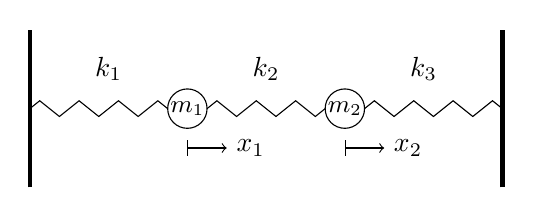
\begin{tikzpicture}
            %\draw[lightgray] (0, 0) grid (6, 2);
            \draw (2, 1) circle (0.25);
            \draw (4, 1) circle (0.25);
            \draw[decoration={zigzag, segment length = 0.5cm, amplitude = 0.1cm}, decorate] (0, 1) -- (1.75, 1);
            \draw[decoration={zigzag, segment length = 0.5cm, amplitude = 0.1cm}, decorate] (2.25, 1) -- (3.75, 1);
            \draw[decoration={zigzag, segment length = 0.5cm, amplitude = 0.1cm}, decorate] (4.25, 1) -- (6, 1);
            \draw[ultra thick] (0, 0) -- (0, 2);
            \draw[ultra thick] (6, 0) -- (6, 2);
            \node at (2, 1) {\small\(m_1\)};
            \node at (4, 1) {\small\(m_2\)};
            \node at (1, 1.5) {\(k_1\)};
            \node at (3, 1.5) {\(k_2\)};
            \node at (5, 1.5) {\(k_3\)};
            \draw[|->] (2, 0.5) -- (2.5, 0.5);
            \draw[|->] (4, 0.5) -- (4.5, 0.5);
            \node[right] at (2.5, 0.5) {\(x_1\)};
            \node[right] at (4.5, 0.5) {\(x_2\)};
        \end{tikzpicture}
        \caption{Coupled mass spring system}
        \label{fig:mass spring coupled system}
    \end{figure}
    Figure \ref{fig:mass spring coupled system} shows a coupled mass--spring system.
    We define \(x_1 = x_2 = 0\) when the system is at equilibrium.
    We can consider the forces on each mass.
    Starting with \(m_1\) the forces are:
    \begin{itemize}
        \item Force due to spring one: \(-k_1x_1\)
        \item Force due to spring two: \(k_2(x_2 - x_1)\)
    \end{itemize}
    and then \(m_2\):
    \begin{itemize}
        \item Force due to spring two: \(-k_2(x_2 - x_1)\)
        \item Force due to spring three: \(-k_3 x_2\)
    \end{itemize}
    This gives us two different equations using Newton's second law:
    \[m_1\dv[2]{x_1}{t} = -(k_1 + k_2)x_1 + k_2x_2\]
    \[m_2\dv[2]{x_2}{t} = k_2 x_1 - (k_2 + k_3)x_2\]
    These are coupled equations as the two functions \(x_1\) and \(x_2\) appear in both.
    One of the best ways to solve this sort of problem is with matrices.
    Let \(X\in\bb R^{2\times 1}\):
    \[X = \begin{pmatrix} x_1 \\ x_2 \end{pmatrix}\]
    Let \(M, K\in\bb R^{2\times 2}\) such that
    \begin{equation}\label{eqn:matrix N2 for mass spring}
        M\dv[2]{X}{t} = -KX
    \end{equation}
    By inspection we can see that
    \[
        M = 
        \begin{pmatrix}
            m_1 & 0 \\ 0 & m_2
        \end{pmatrix}
    \]
    \[
        K = 
        \begin{pmatrix}
            k_1 + k_2 & -k_2 \\ -k_2 & k_2 + k_3
        \end{pmatrix}
    \]
    We make the ansatz that \(X = Ce^{i\omega t}\) for \(C\in\bb R^{2\times 1}\) and \(\omega\in\bb R\).
    Substituting this into equation \ref{eqn:matrix N2 for mass spring} we get
    \[(K - \omega^2M)X = 0\]
    For this to be true for all \(X\) we need
    \[|K-\omega^2 M| = 0\]
    We define \(\lambda = \omega^2\) and we get that this determinant is
    \[
        \begin{vmatrix}
            k_1 + k_2 - \lambda m_1 & -k_2\\
            -k_2 & k_2 + k_3 - \lambda m_2
        \end{vmatrix}
        = (k_1 + k_2 - \lambda m_1)(k_2 + k_3 - \lambda m_2) - k_2^2 = 0
    \]
    \[m_1m_2\lambda^2 - [(k_1 + k_2)m_2 + (k_2 + k_3)m_1]\lambda + (k_1 + k_2)(k_2 + k_3) = 0\]
    This is a quadratic in \(\lambda\) and can be solved to find \(\lambda\) and hence \(\omega^2\) and \(X\).
    For ease we will consider the case where \(m_1 = m_2 = m\) and \(k_1 = k_2 = k_3 = k\).
    Then the quadratic reduces to
    \[(m\lambda - 3k)(m\lambda - k) = 0\]
    This gives two values of \(\lambda\):
    \[\lambda_A = \omega_A^2 = \frac{k}{m},\qquad \lambda_B = \omega_B^2 = \frac{3k}{m}\]
    These two values of \(\lambda\) relate to the fact that there are two modes of oscillation.
    Each mode represents one way of oscillating and the resultant oscillation is a linear combination of all of the modes.
    
    We can substitute these nodes into the eigenvalue equation
    \[(-\lambda M + K)X = 0\]
    This gives similar equations for the top and bottom lines of the matrices.
    The first is
    \[(-\lambda m + 2k)x_1 -kx_2 = 0\implies \frac{x_2}{x_1} = \frac{-m\lambda + 2k}{k}\]
    If we substitute in \(\lambda_A = k/m\) we get
    \[x_1 = x_2\]
    This corresponds to spring two having a constant length and masses one and two moving backwards and forwards in phase.
    If instead we substitute \(\lambda_B = 3k/m\) we get
    \[x_1 = -x_2\]
    This corresponds to the two masses being exactly \(\pi\) radians out of phase and moving together and then apart.
    We can solve for the eigenvectors \(X\) and we get
    \[X_A = \frac{\sqrt{2}}{2}\begin{pmatrix} 1 \\ 1 \end{pmatrix}\]
    \[X_B = \frac{\sqrt{2}}{2}\begin{pmatrix} 1 \\ -1 \end{pmatrix}\]
    The two modes of oscillation can describe the motion of \(m_1\) in the following equations:
    \[x_1 = C_Ae^{i\omega_A t},\qquad x_1 = C_Be^{i\omega_B t}\]
    And then the relationship between \(x_1\) and \(x_2\) for each mode gives the equation of motions for \(x_2\) under each mode as
    \[x_2 = C_Ae^{i\omega_A t},\qquad x_2 = -C_Be^{i\omega_B t}\]
    These two equations for each mass are then added together to give the total equations of motion for each mass as
    \[2x_1 = C_Ae^{i\omega_A t} + C_Be^{i\omega_B t},\qquad 2x_2 = C_Ae^{i\omega_A t} - C_Be^{i\omega_B t}\]
    
    \subsection{Coupled Pendulums}
    Two pendulums of mass \(m\) with angles \(\vartheta_1\) and \(\vartheta_2\) are coupled by a spring of spring constant \(k\).
    The horizontal displacement of the pendulums from equilibrium is given by \(x_1\) and \(x_2\) respectively.
    Newton's second law for the two pendulums is
    \[m\dv[2]{x_1}{t} = -m\omega_0^2x_1 + k(x_2 - x_1)\]
    \[m\dv[2]{x_2}{t} = -m\omega_0^2x_2 - k(x_2 - x_1)\]
    We make the ansatz that
    \[x_1 = Ae^{i\omega t},\qquad x_2 = Be^{i\omega t}\]
    Differentiating and substituting in we get
    \[-m\omega^2 A + m\omega_0^2A + k(A - B) = 0\]
    \[-m\omega^2 B + m\omega_0^2 B - k(A - B) = 0\]
    The first solution to this is \(\omega_1 = \omega_0\) and \(A = B\).
    This corresponds to the normal motion of the pendulums, in phase, with the spring having constant length.
    The second solution is
    \[\omega_2 = \sqrt{\omega_0^2 + \frac{2k}{m}}\]
    and \(A = -B\).
    This corresponds to the pendulums being exactly \(\pi\) radians out of phase and at some slightly higher frequency than the natural frequency.
    
    \subsection{\ce{CO2} molecule}
    A \ce{CO2} molecule behaves very similarly to three masses attached in a line by two springs with spring constants \(k\).
    The middle mass, \(m_C\), is the carbon atom and the outer two masses, \(m_O\), are the oxygen atoms.
    The displacement, along the bond axis, from equilibrium is given by \(x_1\), \(x_2\) and \(x_3\) for the three atoms as you move along the molecule.
    We define the quantity
    \[\mu = \frac{m_C}{m_O}\]
    Like before we can create mass and spring constant matrices to simplify the equations of motion.
    These matrices \(M, K\in\bb R^{3\times 3}\) are
    \[
        M = m_0
        \begin{pmatrix}
            1 & 0 & 0\\
            0 & \mu & 0\\
            0 & 0 & 1
        \end{pmatrix}
        ,\qquad
        K = k
        \begin{pmatrix}
            1 & -1 & 0\\
            -1 & 2 & -1\\
            0 & -1 & 1
        \end{pmatrix}
    \]
    We then need to solve
    \[|K - \lambda M| = 0\]
    This gives three solutions for the three modes of oscillation:
    \begin{itemize}
        \item Pure translation, the springs have constant length and there is no oscillation (ie \(\omega = 0\)).
        \item The carbon atom stays stationary and the oxygen atoms move exactly out of phase with each other.
        \[\omega = \sqrt{\frac{k}{m_O}}\]
        \item The oxygen atoms move in one direction and the carbon atom moves in the opposite direction to conserve momentum.
        \[\omega = \sqrt{\frac{k}{m_O} + \frac{2k}{m_C}}\]
    \end{itemize}
    
    \section{More on Coupled Oscillations}
    Recall the mass spring system shown in figure \ref{fig:mass spring coupled system}. When \(k_1 = k_2 = k_3\) and \(m_1 = m_2 = m\).
    We have already shown that the solutions is a linear superposition of the two modes giving
    \[X = AX_Ae^{-i(\omega_A t + \delta_A)} + BX_Be^{-i(\omega_B t + \delta_B)}\]
    for some unknown phase differences \(\delta_A\) and \(\delta_B\) and constants \(A\) and \(B\).
    Splitting this into two equations we get
    \[x_1 = Ae^{-i(\omega_A t + \delta_A)} + Be^{-i(\omega_B t + \delta_B)}\]
    \[x_2 = Ae^{-i(\omega_A t + \delta_A)} - Be^{-i(\omega_B t + \delta_B)}\]
    since the eigenvectors of the two modes differ only by a minus sign in front of the \(x_2\) component.
    We have the initial conditions that at \(t = 0\) \(x_1 = A_0\), \(x_2 = 0\) and \(v_1 = v_2 = 0\) where \(A_0\) is the maximum amplitude of \(m_1\) and \(v_i = \dot x_i\).
    Adding together the two equations, for \(x_1\) and \(x_2\), at \(t = 0\) we get
    \[A_0 = 2Ae^{-i\delta_A} \implies A = \frac{A_0}{2}e^{i\delta_A}\]
    Subtracting instead we get
    \[A_0 = 2Be^{-i\delta_B} \implies B = \frac{A_0}{2}e^{i\delta_B}\]
    This gives \(x_1\) and \(x_2\) as
    \[x_1 = \frac{A_0}{2}(e^{-i\omega_A t} + e^{-i\omega_B t})\]
    \[x_2 = \frac{A_0}{2}(e^{-i\omega_A t} - e^{-i\omega_B t})\]
    since the \(e^{i\delta_j}\) term in the constant cancels with the \(e^{-i\delta_j}\) term in the exponent.
    We define the average frequency as
    \[\overline\omega = \frac{1}{2}(\omega_A + \omega_B)\]
    and the beats frequency as
    \[\Delta\omega = \frac{1}{2}(\omega_A - \omega_B)\]
    The modal frequencies can then be written as
    \[\omega_A = \overline\omega + \Delta\omega,\qquad \omega_B = \overline\omega - \Delta\omega\]
    This allows us to write \(x_1\) and \(x_2\) as
    \[x_1 = \frac{A_0}{2}e^{i\overline\omega t}(e^{-i\Delta\omega t} + e^{i\Delta\omega t})\]
    \[x_2 = \frac{A_0}{2}e^{i\overline\omega t}(e^{-i\Delta\omega t} - e^{i\Delta\omega t})\]
    Using
    \[e^{-i\vartheta} = \cos\vartheta - i\sin\vartheta = \cos\vartheta + e^{3i\pi/2}\sin\vartheta\]
    we can write this as
    \[x_1 = A_0e^{i\overline\omega}\cos(\Delta\omega t)\]
    \[x_2 = A_0e^{i(\overline\omega + 3\pi/2)}\sin(\Delta\omega t)\]
    The exponential term has a larger frequency than the trig term.
    The exponential term causes oscillations and the trig term causes the amplitude of these oscillations to oscillate.
    \begin{figure}[ht]
        \centering
        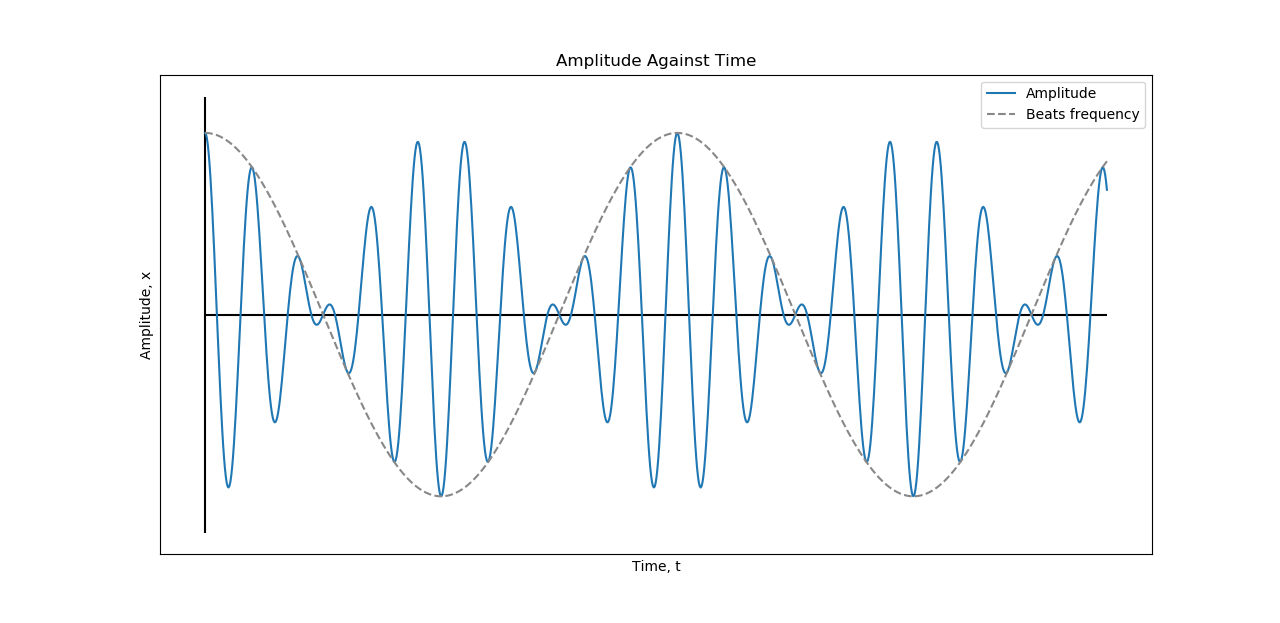
\includegraphics[scale=0.5]{beats_frequency.png}
        \caption{A graph of the amplitude of the oscillator as well as the oscillation of the amplitude}
    \end{figure}

    \subsection{Energy Conservation}
    Consider the mass spring system shown in figure \ref{fig:mass spring coupled system} where \(k_1 = k_3\) and \(m_1 = m_2 = m\) .
    We want to show that the energy of each mode is conserved individually.
    The solution to this is \(\lambda_A = \omega_A^2 = k_1/m\) and \(\lambda_B = \omega_B^2 = (k_1 + 2k_2)/m\).
    The eigenvectors are
    \[
        x_A = \frac{\sqrt{2}}{2}
        \begin{pmatrix}
            1 \\ 1
        \end{pmatrix}
        ,\qquad
        x_B = \frac{\sqrt{2}}{2}
        \begin{pmatrix}
            1 \\ -1
        \end{pmatrix}
    \]
    The kinetic and potential energy is given by
    \[T = \frac{1}{2}mA^2\omega^2,\qquad V = \frac{1}{2}kx^2\]
    We will start with mode \(A\).
    The kinetic energy is at a maximum at the equilibrium position \(x_1 = x_2 = 0\).
    It is a minimum and zero at the instance when the masses are instantaneously at rest at the amplitude \(x_1 = x_2 = A\).
    The difference between these two points is
    \[\Delta T = T_\text{max} - T_\text{min} = 2\frac{1}{2}mA^2\omega_A^2 = mA^2\omega_A^2 = k_1A^2\]
    where we have used \(k_1 = m\omega_A^2\) which comes from \(m\ddot x_1 = -k_1 x_1\) and \(x_1 = e^{i\omega_A} \implies \ddot x_1 = -\omega_A^2x_1\).
    The potential energy is at a maximum at the amplitude \(x_1 = x_2 = A\) and is at a minimum and zero when \(x_1 = x_2 = 0\).
    The difference between these two points is
    \[\Delta V = V_\text{max} - V_\text{min} = 2\frac{1}{2}k_1A^2 = k_1A^2\]
    Since the maximum kinetic energy and minimum potential energy occur at the same time and vice versa the total energy at either time is \(k_1A^2\) so energy is conserved (at least at these two points).
    We can do the same for mode \(B\).
    The maximum kinetic energy now occurs at \(x_1 = x_2 = 0\).
    Since the masses are moving in different directions the kinetic energies are
    \[\Delta T = 2\frac{1}{2}mA^2\omega_B^2 = mA^2\omega_B^2\]
    The maximum potential energy now occurs at \(x_1 = -x_2 = A\).
    The minimum potential energy is the same.
    \[\Delta V = 2\frac{1}{2}(k_1A^2 + 2k_2(-A)^2) = A^2(k_1 + 2k_2)\]
    The \(k_1\) term comes from the extension of the outer springs and the \(k_2\) term from the extension of the inner spring due to \(x_1\) and \(x_2\) (hence the factor of 2).
    \(\Delta T = \Delta V\) if \(\omega_B^2 = (k_1 + 2k_2)/m\) which it does.
    
    In fact it turns out that each mode always conserves energy individually and that the higher frequency modes have more energy in general.
    We can show this more generally with matrices.
    
    In this section upright bold will be used to represent a matrix, eg \(\mat M\), \(\mat K\) and \(\mat x_i\).
    We use the normal coordinates \(\mat x_i\in\bb R^{2\times1}\) for each mode.
    The kinetic energy is given by
    \[T = \frac{1}{2}\left(\dv{\mat x_i}{t}\right)\trans\mat M \left(\dv{\mat x_i}{t}\right)\]
    where \(\mat M\in\bb R^{2\times2}\) is
    \[\mat M = \begin{pmatrix}
        m_1 & 0\\
        0 & m_2
    \end{pmatrix}\]
    Note \(\mat M\) is symmetric.
    The potential energy is given by
    \[V = \frac{1}{2}\mat x_i\trans\mat K\mat x_i\]
    where \(\mat K\in\bb R^{2\times2}\) is
    \[\mat K = \begin{pmatrix}
        k_1 + k_2 & -k_2\\
        -k_2 & k_1 + k_2
    \end{pmatrix}\]
    Note \(\mat K\) is symmetric.
    To show that energy is conserved we show that
    \[\dv{E}{t} = \dv{t}[T + V] = 0\]
    \[\dv{t}T = \frac{1}{2}\left(\dv[2]{\mat x_i}{t}\right)\trans\mat M\left(\dv{\mat x_i}{t}\right) + \frac{1}{2}\left(\dv{\mat x_i}{t}\right)\trans\mat M\left(\dv[2]{\mat x_i}{t}\right)\]
    \[\dv{t}V = \frac{1}{2}\left(\dv{\mat x_i}{t}\right)\trans\mat K\mat x_i + \frac{1}{2}\mat x_i\trans\mat K\left(\dv{\mat x_1}{t}\right)\]
    Combining and factoring out \(\dd\mat x_i/\dd t\) and \((\dd\mat x_i/\dd t)\trans\) where appropriate we get
    \[\dv{E}{t} = \frac{1}{2}\left(\dv{\mat x_i}{t}\right)\trans\left[\mat M\left(\dv[2]{\mat x_i}{t}\right) + \mat K\mat x_i\right] + \frac{1}{2}\left[\left(\dv[2]{\mat x_i}{t}\right)\trans\mat M + \mat x_i\trans\mat K\right]\left(\dv{\mat x_i}{t}\right)\]
    The first term is the transpose of the second and the first term is zero since by Newton's second law we started with
    \[\mat M\left(\dv[2]{\mat x_i}{t}\right) = -\mat K\mat x_i\]
    This means that the rate of change of energy is zero so energy is conserved.
    
    \subsection{Double Pendulum}\label{sec:double pendulum}
    Energy conservation can also be used to find equations of motion.
    For example a double pendulum as shown in figure \ref{fig:double pendulum}
    \begin{figure}[ht]
        \centering
        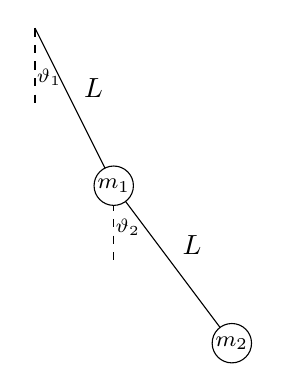
\begin{tikzpicture}
            \draw (0, 4) -- (1, 2);
            \draw (1, 2) -- (2.5, 0);
            \draw[dashed] (0, 4) -- (0, 3);
            \draw[dashed] (1, 2) -- (1, 1);
            \draw[fill=white] (1, 2) circle (0.25);
            \draw[fill=white] (2.5, 0) circle (0.25);
            \node at (1, 2) {\footnotesize\(m_1\)};
            \node at (2.5, 0) {\footnotesize\(m_2\)};
            \node[below right] at (-0.1, 3.6) {\scriptsize\(\vartheta_1\)};
            \node[below right] at (0.9, 1.7) {\scriptsize\(\vartheta_2\)};
            \node[above right] at (0.5, 3) {\(L\)};
            \node[above right] at (1.75, 1) {\(L\)};
        \end{tikzpicture}
        \caption{A double pendulum}
        \label{fig:double pendulum}
    \end{figure}
    The trouble with the Newton's second law approach to this problem is that there is no nice set of coordinates to describe the position of both masses.
    This means that vectors are not the ideal approach.
    Conservation of energy allows us to use scalars instead.
    We start by defining zero potential energy as \(\vartheta_1 = \vartheta_2 = 0\).
    At any point in time the first mass is \(L - L\cos\vartheta_1\) above this equilibrium position.
    Likewise the second mass is higher due to its pivot at mass one being higher and due to the angle it is at, its height above equilibrium is \(L - L\cos\vartheta_1 + L - L\cos\vartheta_2\).
    The potential energy is the
    \[V = m_1g(L - L\cos\vartheta_1) + m_2g(L - L\cos\vartheta_1 + L - L\cos\vartheta_2)\]
    This can be simplified using the small angle approximation we get \(L - L\cos\vartheta \approx L - L(1 - \vartheta^2/2) = L\vartheta^2/2\)
    \begin{align*}
        V &= m_1g\frac{L\vartheta_1^2}{2} + m_2g\left[\frac{L\vartheta_1^2}{2} + \frac{L\vartheta_2^2}{2}\right]\\
        &= \frac{gL}{2}\left[m_1\vartheta_1^2 + m_2(\vartheta_1^2 + \vartheta_2^2)\right]
    \end{align*}
    The kinetic energy is slightly trickier.
    The kinetic energy of the first mass is
    \[T_1 = \frac{1}{2}m_1L^2\left(\dv{\vartheta_1}{t}\right)^2\]
    since \(v_1 = L\omega_1 = L\dot\vartheta_1\).
    To find the kinetic energy of the second pendulum we consider its \(x\) and \(y\) velocities.
    \[x_2 = L\sin\vartheta_1 + L\sin\vartheta_2\]
    \[y_2 = L\cos\vartheta_1 + L\cos\vartheta_2\]
    \[\dv{x_2}{t} = L\left[\cos\vartheta_1\dv{\vartheta_1}{t} + \cos\vartheta_2\dv{\vartheta_2}{t}\right]\]
    \[\dv{y_2}{t} = -L\left[\sin\vartheta_1\dv{\vartheta_1}{t} + \sin\vartheta_2\dv{\vartheta_2}{t}\right]\]
    The kinetic energy of the second pendulum is then
    \begin{align*}
        T_2 &= \frac{1}{2}m_2\left[\left(\dv{x_2}{t}\right)^2 + \left(\dv{y_2}{t}\right)^2\right]\\
        &= \frac{1}{2}m_2L^2\left[\cos^2\vartheta_1\left(\dv{\vartheta_1}{t}\right)^2 + \cos^2\vartheta_2\left(\dv{\vartheta_2}{t}\right)^2 + 2\cos\vartheta_1\cos\vartheta_2\dv{\vartheta_1}{t}\dv{\vartheta_2}{t}\right.\\
        &\hphantom{=\frac{1}{2}m_2L^2[]} + \left.\sin^2\vartheta_1\left(\dv{\vartheta_1}{t}\right)^2 + \sin^2\vartheta_2\left(\dv{\vartheta_2}{t}\right) + 2\sin\vartheta_1\sin\vartheta_2\dv{\vartheta_1}{t}\dv{\vartheta_2}{t}\right]\\
        &= \frac{1}{2}m_2L^2\left[\left(\dv{\vartheta_1}{t}\right)^2 + \left(\dv{\vartheta_2}{t}\right)^2 + 2\dv{\vartheta_1}{t}\dv{\vartheta_2}{t}\,\! (\cos\vartheta_1\cos\vartheta_2 + \sin\vartheta_1\sin\vartheta_2)\right]
    \end{align*}
    Using \(\cos\vartheta_1\cos\vartheta_2 + \sin\vartheta_1\sin\vartheta_2 = \cos(\vartheta_1 - \vartheta_2)\), since \(\vartheta_1\) and \(\vartheta_2\) are small \(\vartheta_2 - \vartheta_1\) is also small so to first order \(\cos(\vartheta_2 - \vartheta_2) = 1 + \mathcal O ((\vartheta_2 - \vartheta_1)^2)\)
    \[T_2 = \frac{1}{2}m_2L^2\left[\left(\dv{\vartheta_1}{t}\right)^2 + \left(\dv{\vartheta_2}{t}\right)^2 + 2\dv{\vartheta_1}{t}\dv{\vartheta_2}{t}\right]\]
    The total kinetic energy is then
    \[T = T_1 + T_2 = \frac{1}{2}L^2\left[m_1\left(\dv{\vartheta_1}{t}\right)^2 + m_2\left(\left(\dv{\vartheta_1}{t}\right)^2 + \left(\dv{\vartheta_2}{t}\right)^2 + 2\dv{\vartheta_1}{t}\dv{\vartheta_2}{t}\right)\right]\]
    This can be written in matrix form using coordinates \(\vartheta_i\) as
    \[T = \frac{1}{2}L^2\left(\dv{\vartheta_i}{t}\right)\trans\mat M_T\left(\dv{\vartheta_i}{t}\right)\]
    where \(\mat M_T\in\bb R^{2\times2}\) is
    \[\mat M_T = \begin{pmatrix}
        m_1 + m_2 & m_2\\
        m_2 & m_2
    \end{pmatrix}\]
    Likewise the potential energy can be written in matrix form as
    \[V = \frac{1}{2}gL\vartheta_i\trans\mat M_V\vartheta_i\]
    where \(\mat M_V\in\bb R^{2\times2}\) is
    \[\mat M_V = \begin{pmatrix}
        m_1 + m_2 & 0\\
        0 & m_2
    \end{pmatrix}\]
    We can take the time derivative of \(T\) and \(V\) to get
    \[\dv{T}{t} = \frac{1}{2}L^2\left[\left(\dv[2]{\vartheta_i}{t}\right)\trans\mat M_T\left(\dv{\vartheta_i}{t}\right) + \left(\dv{\vartheta_i}{t}\right)\trans \mat M_T\left(\dv[2]{\vartheta_i}{t}\right)\right]\]
    \[\dv{V}{t} = \frac{1}{2}gL\left[\left(\dv{\vartheta_i}{t}\right) \trans\mat M_V\vartheta_i + \vartheta_i\trans\mat M_V \left(\dv{\vartheta_i}{t}\right)\right]\]
    Adding these together we get the total rate of change of energy which we know is zero.
    We factor out \(\dd\vartheta_i/\dd t\) and \((\dd\vartheta_i/\dd t)\trans\) as appropriate to get
    \[0 = \dv{E}{t} = \dv{T}{t} + \dv{V}{t}\]
    \begin{align*}
        0 &= \left(\dv{\vartheta_i}{t}\right)\trans\left[\frac{L^2}{2}\mat M_T\left(\dv[2]{\vartheta_i}{t}\right) + \frac{gL}{2}\mat M_V\vartheta_i\right] + \left[\frac{L^2}{2}\left(\dv[2]{\vartheta_i}{t}\right)\trans\mat M_T + \frac{gL}{2}\vartheta_i\trans\mat M_V\right]\left(\dv{\vartheta_i}{t}\right)
    \end{align*}
    Note that since \(\mat M_T\) and \(\mat M_V\) are symmetric the first term is the transpose of the second.
    So for energy to be conserved we require that
    \[\frac{L^2}{2}\mat M_T\dv[2]{\vartheta_i}{t} + \frac{gL}{2}\mat M_V\vartheta_i = 0\]
    This gives the equation of motion
    \[\mat M_T\dv[2]{\vartheta_i}{t} + \frac{g}{L}\mat M_V\vartheta_i = 0\]
    We assume that \(\vartheta_i = \mat Ce^{i\omega t}\) for \(\mat C\in\bb R^{2\times1}\).
    This gives \(\ddot\vartheta_i = -\omega^2\vartheta_i = -\lambda\vartheta_i\).
    From this we can see that
    \[\left(\frac{g}{L}\mat M_V - \lambda\mat M_T\right)\vartheta_i = 0\]
    For this to be true for all \(\vartheta_i\) we need
    \[\left|\frac{g}{L}\mat M_V - \lambda\mat M_T\right| = 0\]
    \[
        \left|\frac{g}{L}
        \begin{pmatrix}
            m_1 + m_2 & 0\\
            0 & m_2
        \end{pmatrix}
        - \lambda
        \begin{pmatrix}
            m_1 + m_2 & m_2\\
            m_2 & m_2
        \end{pmatrix}
        \right| = 0
    \]
    \[
    \begin{vmatrix}
        (m_1 + m_2)\left(\frac{g}{L} - \lambda\right) & -m_2\lambda\\
        -m_2\lambda & m_2\left(\frac{g}{L} - \lambda\right)
    \end{vmatrix}
    = 0
    \]
    \[m_2(m_1 + m_2)\left(\frac{g}{L} - \lambda\right)^2 - m_2^2\lambda^2 = 0\]
    we will consider the case where \(m_1 = m_2 = m\) to simplify this further.
    \[2m^2\left(\lambda^2 - 2\frac{g}{L}\lambda + \frac{g^2}{L^2}\right) - m^2\lambda^2 = 0\]
    \[\lambda^2 - 2\frac{g}{L}\lambda + 2\frac{g^2}{L^2} = 0\]
    \[\lambda_i = \omega_i^2 = \frac{g}{L}(2\pm\sqrt{2})\]
    The eigenvectors are
    \[\vartheta_A = \frac{\sqrt{3}}{3}\begin{pmatrix} 1 \\ \sqrt{2}\end{pmatrix},\qquad \vartheta_B = \frac{\sqrt{3}}{3}\begin{pmatrix}1 \\ -\sqrt{2}\end{pmatrix}\]
    
    \part[Orbits and Scattering]{Orbits and Scattering\\[\bigskipamount]\large Central Forces, Angular Momentum, Orbit Equation, Kepler's Laws, Precession, Hyperbolic Orbits, Scattering, Hard-body Scattering, Rutherford Scattering}
    
    \section{Central Forces}
    \subsection{Central Force Properties}
    A central force \(\vv F(\vv r)\) is a force such that \(\vv F(\vv r) = F(r)\vh r\) that is the strength of the force only depends on the distance from the origin and the direction is always \(\vh r\).
    Such a force has curl given by
    \[\curl\vv F(\vv r) = \curl(F(r)\vh r) = (\grad F(r))\times\vh r + F(r)(\curl\vh r) = \frac{F'(r)}{r}\vh r\times\vh r + F(r)(\curl\vh r) = \vv 0\]
    Since the curl is always zero there exists a potential \(V(\vh r)\) such that \(\vv F(\vv r) = -\grad V(\vh r)\).
    To be able to use Newton's second law with a central force we want to know the acceleration.
    To find this we need the velocity.
    \[\vv v = \dv{\vv r}{t} = \dv{t}[r\vh r] = \dv{r}{t}\vh r + r\dv{\vh r}{t}\]
    recall the derivatives of the polar unit vectors:
    \[\dv{\vh r}{t} = \dv{\vartheta}{t}\vh\vartheta,\qquad \dv{\vh\vartheta}{t} = -\dv{\vartheta}{t}\vh r\]
    Using these the velocity is
    \[\vv v = \dv{r}{t}\vh r + r\dv{\vartheta}{t}\vh \vartheta\]
    The acceleration is then
    \[\vv a = \dv{\vv v}{t} = \dv[2]{r}{t}\vh r + \dv{r}{t}\dv{\vh r}{t} + \dv{r}{t}\dv{\vartheta}{t}\vh \vartheta + r\dv[2]{\vartheta}{t}\vh\vartheta + r\dv{\vartheta}{t}\dv{\vh\vartheta}{t}\]
    \[\vv a = \dv[2]{r}{t}\vh r + \dv{r}{t}\dv{\vartheta}{t}\vh\vartheta + \dv{r}{t}\dv{\vartheta}{t}\vh \vartheta + r\dv[2]{\vartheta}{t}\vh\vartheta - r\dv{\vartheta}{t}\dv{\vartheta}{t}\vh r\]
    \[\vv a = \left[\dv[2]{r}{t} - r\left(\dv{\vartheta}{t}\right)^2\right] + \left[r\dv[2]{\vartheta}{t} + 2\dv{r}{t}\dv{\vartheta}{t}\right]\]
    A central force only has a component in the \(\vh r\) direction.
    \[a_r = \frac{F(r)}{m} = \dv[2]{r}{t} - r\left(\dv{\vartheta}{t}\right)^2 = \dv[2]{r}{t} - r\omega^2\]
    where \(\omega = \dd\vartheta/\dd t\).
    This is like \(a = F/m\) but we are in a non--inertial frame so there is a fictitious force \(-mr\omega^2\) acting.
    The \(\vh\vartheta\) component of acceleration must be zero
    \[a_\vartheta = 0 = r\dv{\omega}{t} + 2\omega\dv{r}{t} = \frac{1}{r}\left[r^2\dv{\omega}{t} + 2r\omega\dv{r}{t}\right] = \frac{1}{r}\dv{t}[r^2\omega]\]
    for this to be zero we require \(r^2\omega\) to be constant.
    This comes from conservation of angular momentum \(L = mr\omega^2\).
    The angular momentum is
    \[\vv L = m\vv r\times(\vv\omega\times\vv r) = m\vv r\times\vv v = \vv r\times\vv p\]
    We can show that this is conserved for a central force:
    \[\dv{\vv L}{t} = \dv{\vv r}{t}\times\vv p + \vv r\times\dv{\vv p}{t} = \vv v\times m\vv v + \vv r\times\vv F = \vv 0\]
    this is zero as any vector crossed with itself is zero and \(\vv F = F\vh r\).
    So angular momentum is conserved.
    
    \subsection{Moment of Inertia and Torque}
    The moment of inertia is defined as the tensor \(I\) such that
    \[\vv L = I\vv\omega\]
    In this course we will almost always consider the case where \(I\) is a scalar.
    The moment of inertia is analogous to the mass in that \(\vv L = I\vv\omega\) is analogous to \(\vv p = m\vv v\).
    The torque, \(\vv\tau\), is defines as
    \[\vv\tau = \dv{\vv L}{t}\]
    hence the torque is analogous to a force in that \(\vv\tau = \dd\vv L/\dd t\) is analogous to \(\vv F = \dd\vv p/\dd t\).
    \[\vv\tau = \dv{\vv L}{t} = \dv{\vv r}{t}\times\vv p + \vv r\times\dv{\vv p}{r} = \vv r\times\vv F\]
    \[\vv\tau = \vv r\times\vv F = I\dv{\vv\omega}{t}\]
    This is analogous to \(\vv F = m\vv a\).
    
    \subsection{Energy}
    The kinetic energy is given by
    \[T = \frac{1}{2}mv^2 = \frac{1}{2}m\vv v\cdot\vv v = \frac{1}{2}m\left(\dv{r}{t}\right)^2 + \frac{1}{2}mr^2\omega^2\]
    We define the first term as \(T_r\) which is the kinetic energy due to changing \(r\) and the second term as \(T_\vartheta\) which is the kinetic energy due to changing \(\vartheta\).
    We can use the angular momentum to find \(\omega\) in terms of \(r\):
    \[L = mr^2\omega\implies \omega = \frac{L}{mr^2}\]
    This allows us to rewrite the second term as
    \[T_\vartheta = \frac{1}{2}mr^2\frac{L^2}{m^2r^4} = \frac{L^2}{2mr^2}\]
    The total energy is
    \[E = V(r) + T_\vartheta + T_r = V(r) + \frac{L^2}{2mr^2} + \frac{1}{2}m\left(\dv{r}{t}\right)^2\]
    We define an effective potential \(V_\text{eff} = V(r) + T_\vartheta\) which controls \(r\) in the same way that a potential controls \(x\) in a one dimensional Cartesian problem.
    
    \subsection{Orbital Motion}
    Orbital motion will occur for a force of the form
    \[F(r) = \frac{K}{r^2}\]
    for some constant \(K\).
    We can find the potential \(V(r)\) as
    \[V(r) = -\int_r^\infty F(r')\,\dd r' = -\frac{K}{r}\]
    where we have chosen to define \(V(\infty) = 0\).
    The acceleration at a distance \(r\) is
    \[\dv[2]{r}{t} = -\frac{K}{mr^2} + r\omega^2 = -\frac{K}{mr^2} + \frac{L^2}{m^2r^3}\]
    This is a non--linear differential equation in \(r\).
    We will solve this with the substitution \(u = 1/r\).
    \[\dv{r}{t} = -\frac{1}{u^2}\dv{u}{t}\]
    \[\dv{u}{t} = \dv{\vartheta}{t}\dv{t}{\vartheta} = \omega\dv{u}{\vartheta}\]
    \[\dv{r}{t} = -\frac{\omega}{u^2}\dv{u}{\vartheta}\]
    using \(\omega = L/mr^2 = Lu^2/m\) this is
    \[\dv{r}{t} = -\frac{L}{m}\dv{u}{\vartheta}\]
    \[\dv[2]{r}{t} = -\frac{L}{m}\dv[2]{u}{\vartheta}\dv{\vartheta}{t} = -\frac{L}{m}\dv[2]{u}{\vartheta}\omega = -\frac{L^2u^2}{m^2}\dv[2]{u}{\vartheta}\]
    substituting into the original differential equation we get
    \[-\frac{L^2u^2}{m^2}\dv[2]{u}{\vartheta} = -\frac{Ku^2}{m} + \frac{L^2u^3}{m^2}\]
    \[-\frac{L^2}{m^2}\dv[2]{u}{\vartheta} = -\frac{K}{m} + \frac{L^2}{m^2}u\]
    \[\dv[2]{u}{\vartheta} + u = \frac{Km}{L^2}\]
    this is the orbit equation.
    We solve it with the ansatz \(u = A\cos\vartheta + B\) (note that we choose a phase of zero)
    \[\dv[2]{u}{\vartheta} = -A\cos\vartheta\]
    \[-A\cos\vartheta + A\cos\vartheta + B = \frac{Km}{L^2}\]
    \[B = \frac{Km}{L^2}\]
    we define two constants
    \[R = \frac{1}{B},\qquad e = \frac{A}{B}\]
    the solution is
    \[u = \frac{1}{r} = \frac{1}{R}(1 + e\cos\vartheta)\]
    \[r = \frac{R}{1 + e\cos\vartheta}\]
    This is the solution to the orbital equation.
    It corresponds to a conic section.
    The shape depends on the value of \(e\):
    \begin{itemize}
        \item \(e = 0\implies A = 0\) - the orbit is a circle
        \item \(0 < e < 1\implies A < B\) - the orbit is elliptical
        \item \(e = 1\implies A = B\) - the orbit is parabolic
        \item \(e > 1\implies A > B\) - the orbit is hyperbolic
    \end{itemize}
    The closest that the orbiting body will get is
    \[\frac{R}{1 + e}\]
    this is known as the pericentre of the orbit.
    An ellipse also has a furthest point that the two bodies will get which is a distance of
    \[\frac{R}{1 - e}\]
    this is known as the apocentre of the orbit.
    A circle or ellipse is a bound orbit and parabolas and hyperbolas are unbound as the ellipse will go to infinity as at some value of \(\vartheta\) \(1 - e\cos\vartheta\) will be zero.
    \section{Orbits and Kepler's Laws}
    \subsection{Energy in Orbit}
    The total energy of an orbiting object in a central force of \(F(r) = -K/r^2\) is
    \[E = \frac{1}{2}m\left(\dv{r}{t}\right)^2 - \frac{K}{r} + \frac{1}{2}\frac{L^2}{mr^2}\]
    As before we substitute \(u = 1/r\) and we get
    \[\dv{r}{t} = -\frac{L}{m}\dv{u}{\vartheta}\]
    Hence the total energy is
    \[E = \frac{L^2}{2m}\left(\dv{u}{\vartheta}\right)^2 - Ku + \frac{L^2u^2}{2m}\]
    this has a minimum when \(r = R\), this point represents the most stable orbital radius which will be the radius at which a circular orbit will be performed.
    
    \subsection{Elliptic Orbits}
    \begin{figure}[ht]
        \centering
        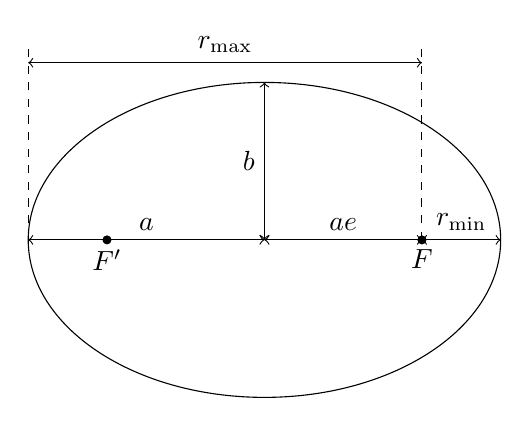
\begin{tikzpicture}
            %\draw[lightgray] (0, 0) grid (6, 6);
            \draw (3, 2) ellipse[x radius=3cm, y radius=2cm];
            \draw[fill=black] (1, 2) circle[radius=0.05cm];
            \draw[fill=black] (5, 2) circle[radius=0.05cm];
            \node[below] at (5, 2) {\(F\)};
            \node[below] at (1, 2) {\(F'\)};
            \draw[<->] (3, 2) -- (3, 4);
            \draw[<->] (3, 2) -- (0, 2);
            \node[left] at (3, 3) {\(b\)};
            \node[above] at (1.5, 2) {\(a\)};
            \draw[<->] (3, 2) -- (5, 2);
            \node[above] at (4, 2) {\(ae\)};
            \draw[<->] (5, 2) -- (6, 2);
            \node[above] at (5.5, 2) {\(r_\text{min}\)};
            \draw[dashed] (5, 2) -- (5, 4.5);
            \draw[dashed] (0, 2) -- (0, 4.5);
            \draw[<->] (0, 4.25) -- (5, 4.25);
            \node[above] at (2.5, 4.25) {\(r_\text{max}\)};
        \end{tikzpicture}
        \caption{Elliptical orbit with its orbital and geometric parameters marked}
    \end{figure}
    An ellipse is the set of all points such that the sum of the distances from the point each focus is a constant.
    In an elliptic orbit the central body is at one focus of the ellipse.
    The geometric parameters of an ellipse are its semimajor axis, \(a\), its semiminor axis, \(b\), and its eccentricity, \(e\).
    \[e^2 = 1 - \frac{b^2}{a^2}\]
    The parameters of the orbit such as \(r_\text{min}\) and \(r_\text{max}\) are related to the geometric parameters by
    \[r_\text{min} = a(1 - e),\qquad r_\text{max} = a(1 + e)\]
    Defining the angle \(\vartheta\) as the angle from the semimajor axis then when \(\vartheta = 0\) we are at \(r_\text{min}\) and
    \[r_\text{min} = \frac{R}{1 + e}\implies a = \frac{R}{1 - e^2}\]
    \[b^2 = a^2(1 - e^2) = \frac{R^2}{(1 - e^2)^2} \implies b \frac{R}{\sqrt{1 - e^2}}\]
    \[R = \frac{B^2}{a}\]
    \[R = \frac{L^2}{Km}\implies L^2 = KmR = Km\frac{b^2}{a}\]
    \[L^2 = m^2r^2v^2 = KmR \implies v^2 = \frac{KR}{mr^2}\]
    For an ellipse the distance oscillates around the minimum potential distance (that is the distance at which the potential is minimal not the distance).
    \[v^2(r_\text{min}) = \frac{KR}{mr_\text{min}^2} = \frac{Kr_\text{min}(1 + e)}{mr_\text{min}^2} = \frac{K(1 + e)}{mr_\text{min}}\]
    \[v^2(r_\text{max}) = \frac{KR}{mr_\text{max}^2} = \frac{Kr_\text{max}(1 - e)}{mr_\text{max}^2} = \frac{K(1 - e)}{mr_\text{max}}\]
    At \(r_\text{min}\) and \(r_\text{max}\) \(\dd r/\dd t = 0\) as \(r\) is at a minimum or maximum.
    This means that the radial kinetic energy term is zero:
    \[T_r = \frac{1}{2}m\left(\dv{r}{t}\right)^2 = 0\]
    Hence the total energy is
    \[E = V(r) + T_\vartheta = -\frac{K}{r} + \frac{1}{2}mv^2\]
    \[E(r_\text{min}) = -\frac{K}{r_\text{min}} + \frac{K(1 + e)}{2r_\text{min}} = \frac{K}{2}\left(\frac{e - 1}{r_\text{min}}\right) = -\frac{K}{2a}\]
    since energy is conserved the total energy anywhere on the orbit must be \(-K/2a\).
    
    \subsection{Kepler's Laws}
    Kepler's laws are laws that Kepler proposed for all orbits.
    They are:
    \begin{enumerate}
        \item Orbits are ellipses with the sun at one focus.
        \item A radius vector from the sun to the planet sweeps out equal areas in equal times.
        If the planet moves at speed \(v\) over time \(\dd t\) it sweeps out an area \(\dd A = r^2\dd\vartheta/2\) hence
        \[\dv{A}{t} = \frac{1}{2}r^2\omega = \frac{L}{2m}\]
        this is constant so the area swept out per unit time is constant.
        \item If the period of an orbit is \(\tau\) and the semimajor axis is \(a\) then \(\tau^2\propto a^3\).
        \[L = mr^2\dv{\vartheta}{t}\implies \int_0^\tau\dd t = \int_0^{2\pi}\frac{m}{L}r^2\,\dd\vartheta = \tau = \frac{m}{L}\int_0^{2\pi}2\,\dd A = \frac{2mA}{L} = \frac{2m\pi ab}{L}\]
        where we have used \(2\dd A = r^2\dd\vartheta\) from before and that \(A = \pi ab\).
        \[L^2 = \frac{Kmb^2}{a}\implies b^2 = \frac{aL^2}{Km}\]
        \[\tau^2 = \frac{4\pi^2m^2}{L^2}a^2b^2 = \frac{4\pi^2m^2}{L^2}a^2\frac{aL^2}{Km} = \frac{4\pi^2m}{K}a^3\]
        so \(\tau^2 \propto a^3\) as we were initially trying to show.
        The \(m\) in the numerator of the prefactor of \(a^3\) cancels with the \(m\) in \(K\) for gravity to make the orbits independent of mass.
    \end{enumerate}
    
    \section{Transfer Orbits and Precession}
    \subsection{Transfer Orbits}
    \begin{figure}[ht]
        \centering
        \begin{tikzpicture}
            \draw (0, 0) circle[radius=1];
            \draw (0, 0) circle[radius=4];
            \draw[dashed] (0, 1.5) ellipse[x radius=1.5, y radius=2.5];
            \draw[->] (0, -1) -- (1.5, -1);
            \draw[->] (0, 4) -- (-1.5, 4);
            \node[right] at (1.5, -1) {\(v_1\)};
            \node[left] at (-1.5, 4) {\(v_2\)};
        \end{tikzpicture}
        \caption{Transfer orbit between two circular orbits}
        \label{fig:transfer orbit}
    \end{figure}
    Figure \ref{fig:transfer orbit} shows a transfer orbit.
    This is the most energy efficient orbit to move from one circular orbit to another.
    Consider the central circular orbit to be that of Earth and the outer to be that of Jupiter.
    The velocity of earth is given by
    \[v_E = \sqrt{\frac{GM_\text{sun}}{R_E}} = \SI{29.8}{km.s^{-1}}\]
    where \(M_\text{sun}\) is the mass of the sun, \(R_E\) is the radius of the orbit of the Earth and \(G\) is the gravitational constant.
    Likewise the velocity of Jupiter is
    \[v_J = \sqrt{\frac{GM_\text{sun}}{R_J}} = \SI{13.1}{km.s^{-1}}\]
    where \(R_J\) is the radius of the orbit of Jupiter.
    The radius of Earth's orbit defines one atomic unit.
    That is \(\SI{1}{AU}\defeq R_E\).
    The radius of Earth's orbit, in terms of the transfer orbit's parameters, is
    \[R_E = a(1 - e) = \SI{1}{AU}\]
    The radius of Jupiter's orbit is
    \[R_J = a(1 + e) = \SI{5.2}{AU}\]
    This gives two simultaneous equations.
    We can solve them and we find that \(a = \SI{3.1}{AU}\) and \(e = 0.677\).
    The velocity squared at \(r_\text{min}\) is \(v^2(r_\text{min})\) and
    \[v^2(r_\text{min}) \propto \frac{1 + e}{r_\text{min}}\]
    The transfer orbit starts with a boost to velocity \(v_1\) given by
    \[v_1 = v_E\sqrt{1 + e} = \SI{38.6}{km.s^{-1}}\]
    this is found by taking the position when leaving Earth to be \(r_\text{min}\) and assuming the orbit of Earth is circular so \(e_E = 0\).
    Therefore the velocity change needed for the first boost is
    \[\Delta v_1 = v_1 - v_E = \SI{8.8}{km.s^{-1}}\]
    Note that this is less than the escape velocity of Earth, as we would expect as the rocket will never be infinitely far away.
    At Jupiter we take the position to be the \(r_\text{max}\) and we find
    \[v^2(r_\text{max}) \propto \frac{1 - e}{r_\text{max}}\]
    We then boost to \(v_2\) to match the velocity of Jupiter.
    \[v_2 = v_J\sqrt{1 - e} = \SI{7.4}{km.s^{-1}}\]
    where we have assumed a circular orbit for Jupiter so \(e_J = 0\).
    This means that the velocity change for the second boost is
    \[\Delta v_2 = v_j - v_2 = \SI{5.7}{km.s^{-1}}\]
    The time period of the orbit is \(\tau\) and is given by
    \[\tau^2 = \frac{4\pi^2a^3}{GM_\text{sun}}\]
    \(\tau = \SI{5.4}{yrs}\).
    So to get from Earth to Jupiter will take half of this time which is \(\SI{2.7}{yrs}\).
    
    \subsection{Two Body Orbits}
    So far we have considered the central body to be fixed.
    If we want to allow all bodies to move then we can do this by considering orbits around the centre of mass of the system.
    There are two bodies of mass \(m_1\) and \(m_2\) at positions \(\vv r_1\) and \(\vv r_2\) respectively.
    The centre of mass of these two bodies is positioned at
    \[\vv R = \frac{m_1\vv r_1 + m_2\vv r_2}{m_1 + m_2}\]
    We choose a coordinate system such that the centre of mass is at the origin.
    We define the vector from body 2 to body 1 as \(\vv r = \vv r_1 - \vv r_2\).
    This allows us to rewrite \(\vv r_1\) and \(\vv r_2\) as
    \[\vv r_1 = \frac{m_2}{m_1 + m_2}\vv r,\qquad \vv r_2 = \frac{m_1}{m_1 + m_2}\vv r\]
    Applying Newton's second law we get
    \[m_1\dv[2]{\vv r_1}{t} = \vv F_1 = F(r)\vh r,\qquad m_2\dv[2]{\vv r_2}{t} = \vv F_2 = -F(r)\vh r\]
    subtracting the second equation from the first we get
    \[2F(r)\vh r = m_1\dv[2]{\vv r_1}{t} - m_2\dv[2]{\vv r_2}{t} = 2\frac{m_1m_2}{m_1 + m_2}\dv[2]{\vv r}{t}\]
    \[F(r)\vh r = \frac{m_1m_2}{m_1 + m_2}\dv[2]{\vv r}{t} = \mu\dv[2]{\vv r}{t}\]
    where \(\mu\) is the reduced mass:
    \[\mu = \frac{m_1m_2}{m_1 + m_2}\]
    This is the same force as for a single body orbit but the mass is replaced with \(\mu\).
    The kinetic energy is
    \[T = \frac{1}{2}\left[m_1\left(\dv{r_1}{t}\right)^2 + m_2\left(\dv{r_2}{t}\right)\right]^2 = \frac{1}{2}\mu\left(\dv{r}{t}\right)^2\]
    Assuming circular orbits the forces are given by \(F_1 = m_1r_1\omega_1^2\) and \(F_2 = m_2r_2\omega_2^2\), since both periods are the same we require \(\omega_1 = \omega_2 = \omega\) so
    \[F_1 = -F_2 = \mu r\omega^2\]
    if the force is gravity then
    \[\omega^2 = \frac{G(m_1 + m_2)}{r^3}\]
    The time period \(\tau\) is given by
    \[\tau^2 = \left(\frac{2\pi}{\omega}\right)^2 = \frac{4\pi^2r^3}{G(m_1 + m_2)}\]
    
    \subsection{Precession}
    If there are more than two bodies but one body is the cause of most of the force acting on each other body, as is the case with the sun in our solar system, then the situation is more complicated.
    This scenario can be modelled as a two body interaction between each body and the sun as well as some perturbation.
    We assume an almost \(1/r^2\) force given by
    \[F = -\frac{K}{r^{2 + \alpha}}\]
    where \(\alpha\) is some small constant.
    Recall that
    \[u^2\dv[2]{u}{\vartheta} + u^3 = \frac{Km}{L^2}u^2\]
    where \(u = 1/r\).
    The factors of \(u^2\) on the left hand side come from the fact that we are working in polar coordinates.
    The factor of \(u^2\) on the right hand side comes from the force.
    For this reason we replace only this term with \(u^{2 + \alpha}\).
    Cancelling \(u^2\) we get
    \[\dv[2]{u}{\vartheta} + u = \frac{u^\alpha}{R}\]
    where \(R = L^2/Km\).
    We assume a solution of the form
    \[u = \frac{1}{R}[1 + \varepsilon(\vartheta)]\]
    where \(\varepsilon(\vartheta)\) is some error term that is \(e\cos\vartheta\) if \(\alpha = 0\).
    This is so that we recover the original orbit equation.
    This differentiating and then plugging into the differential equation we get
    \[\dv[2]{u}{\vartheta} = \frac{1}{R}\dv[2]{\varepsilon}{\vartheta}\]
    \[\frac{1}{R}\dv[2]{\varepsilon}{\vartheta} + \frac{1}{R}(1 + \varepsilon) = \frac{1}{R}\frac{1}{R^\alpha}(1 + \varepsilon)^\alpha\]
    \[\dv[2]{\varepsilon}{\vartheta} + 1 + \varepsilon = \frac{1}{R^\alpha}(1 + \varepsilon)^\alpha\]
    The term on the right can be Taylor expanded if \(\alpha\ll 1\), we also assume that \(R^{-\alpha}\approx 1\).
    \[\dv[2]{\varepsilon}{\vartheta} + 1 + \varepsilon = 1 + \alpha\varepsilon + \mathcal{O}(\alpha^2)\]
    \[\dv[2]{\varepsilon}{\vartheta} = -(1 - \alpha)\varepsilon\]
    we can identify this with SHM with solution
    \[\varepsilon = \frac{1}{R}(1 + e\cos\omega\vartheta),\qquad\omega = \sqrt{1 - \alpha}\]
    This is slightly different to before.
    The orbit no longer ends at \(\vartheta = 2\pi\) but somewhere else slightly further, or earlier, on.
    This causes the whole orbit to process.
    
    \section{Hyperbolic orbits}
    A hyperbola has the equation
    \[\frac{x^2}{a^2} - \frac{y^2}{b^2} = 1\]
    Like an elliptic orbit there are geometric and orbital parameters to a hyperbolic orbit.
    The eccentricity of a hyperbola is \(e\) and is given by \(e^2 = 1 + b^2/a^2\).
    The closest that a particle on an hyperbolic orbit comes to the origin is \(a\).
    The body that it is orbiting is at one of the focuses.
    The closest distance between the two bodies is \(r_\text{min}\).
    The distance from the focus to the origin is \(ae\).
    From this we get 
    \[r_\text{min} = a(e - 1) = \frac{R}{1 + e} \implies a \frac{R}{2^2 - 1}\]
    \[b = \frac{R}{\sqrt{e^2 - 1}}\implies R = \frac{b^2}{a}\]
    as before.
    \(b\) is known as the impact parameter and it is the closest that the two objects would get without the central force that changes the orbit.
    \(\vartheta\) is the deflection angle and is the angle through which the orbit turns.
    \(\vartheta = \pi - 2\alpha\) where \(\alpha\) is the angle from the \(x\) axis to the asymptotes of the hyperbola.
    The two branches of the hyperbola account for the two different orbits that would occur for a repulsive or attractive central force.
    Both \(b\) and \(\vartheta\) are easily measured and are often the two parameters that are chosen to characterise a hyperbolic orbit.
    The angular momentum is given by
    \[L^2 = KmR = \frac{Kmb^2}{a}\]
    The velocity infinitely far away from the body being orbited is \(v_\infty\) and is given by
    \[L^2 = |m\vv r\times\vv v| = mbv_\infty\]
    \[L^" = m^2b^2v_\infty^2 = \frac{Kmb^2}{a}\implies v_\infty^2 = \frac{K}{ma}\]
    At \(r_\text{min}\) \(\dd r/\dd t = 0\) and
    \[L = ma(e - 1)v_\text{min} \implies v_\text{min} = \frac{bv_\infty}{a(e - 1)}\]
    \[v_\text{min}^2 = \frac{b^2 v_\infty^2}{a^2(e - 1)^2} = \frac{(e^2 - 1)v_\infty^2}{(e - 1)^2} = \frac{(e - 1)(e + 1)v_\infty^2}{(e - 1)^2} = \frac{(e^2 + 1)v_\infty^2}{(e - 1)} = \frac{K}{ma}\frac{e + 1}{e - 1}\]
    since \(\dd r/\dd t = 0\) we get
    \[E(r_\text{min}) = -\frac{K}{r_\text{min}} + \frac{1}{2}mv_\text{min}^2 = -\frac{K}{a(e - 1)} + \frac{K}{2a}\frac{e + 1}{e - 1} = \frac{K}{2a(e - 1)}(-2 + e - 1) = \frac{K}{2a}\]
    so, by conservation of energy, the total energy is \(K/2a\) everywhere.
    Note that this is the same as an ellipse but that was negative.
    This is because an ellipse is a bound orbit whereas a hyperbola is an unbound orbit.
    At infinity \(V = 1\) so
    \[E(r_\infty) = \frac{1}{2}mv_\infty^2 = \frac{1}{2}m\frac{K}{ma} = \frac{K}{2a}\]
    as expected.
    Since \(E\) only depends on \(a\) then by specifying \(E\) we specify \(a\) and by specifying \(L\) we can then specify \(b\) since \(L\) only depends on \(a\) and \(b\) and we have already fixed \(a\).
    This means that it is common to talk about orbits in terms of \(E\) and \(L\).
    
    \example
    A comet is in a hyperbolic orbit.
    The velocity of the comet at infinity is given by
    \[v_\infty^2 = \frac{4GM}{3b}\]
    what are the values of \(r_\text{min}\), \(v(r_\text{min})\) and \(\vartheta\)?
    \[E = \frac{K}{2a} = \frac{1}{2}mv_\infty^2\implies v_\infty^2 = \frac{GM}{a}\implies a = \frac{3b}{4}\]
    \[\implies e^2 = 1 + \frac{b^2}{a^2} = \frac{25}{9} \implies e = \frac{5}{3} \implies r_\text{min} = a(e - 1) = \frac{2}{3}a = \frac{b}{2}\]
    \[L = mv(r_\text{min})r_\text{min} = mv_\infty b \implies v(r_\text{min}) = 2v_\infty\]
    \[\frac{b}{a} = \tan\alpha = \frac{4}{3}\implies \alpha = \arctan\frac{4}{3} = \SI{53}{\SIUnitSymbolDegree} \implies \vartheta = \pi - 2\alpha = \SI{74}{\SIUnitSymbolDegree}\]
    
    \section{Scattering}
    \subsection{Differential Cross Sections}\label{sec:diff cross sec}
    The cross section is a measure used in scattering experiments to measure the size of the target area and also the incident particle.
    It is possible to find the cross section by inspection for simple shapes, for example two spheres of radii \(R_1\) and \(R_2\) have a cross section of \(\pi(R_1 + R_2)^2\).
    For more complicated cases we use differential cross sections.
    
    Consider two slightly different trajectories of the incident object.
    One has impact parameter \(b\) and the other \(b + \dd b\).
    Since the second trajectory starts farther out it is deflected less by the object and hence ends up actually being closer to the object.
    The area through which the particles must enter is a ring of width \(\dd b\) and inner radius \(b\):
    \[\dd A_\text{in} = \pi(b + \dd b)^2 - \pi b^2 = \pi(b^2 + 2b\dd b + \dd b^2 - b^2) = 2\pi b\dd b = \dd\sigma\]
    If the deflection angle is \(\vartheta\) then at a distance \(r\) from the target, after scattering, the area in which the objects can be is a ring of width \(r\dd\vartheta\) and inner radius \(r\sin\vartheta\)
    \[\dd A_\text{out} = 2\pi r\sin\vartheta r\dd\vartheta\]
    This corresponds to a solid angle
    \[\dd\Omega = \frac{\dd A_\text{out}}{r^2} = 2\pi\sin\vartheta\dd\vartheta\]
    We define the differential cross section \(\sigma(\vartheta)\) as
    \[\sigma(\vartheta) = -\dv{\sigma}{\Omega} = -\frac{2\pi b\dd b}{2\pi\sin\vartheta\dd\vartheta} = -\frac{b}{\sin\vartheta}\dv{b}{\vartheta}\]
    The negative sign reflects the fact that the particle on the outside ends up on the inside so in a way the area is flipped.
    Note that the derivative \(\dd b/\dd\vartheta < 0\) so \(\sigma(\vartheta) > 0\).
    The total cross section is found by integrating:
    \[\sigma_T = \int_0^{\infty}\dd\sigma = \int_0^\infty 2\pi b\,\dd b = 2\pi\int_0^\pi\sigma(\vartheta)\sin\vartheta\,\dd\vartheta\]
    The limits in the last integral come from the fact that at \(b = 0\) \(\vartheta = \pi\) since the particle bounces right back and at \(b = \infty\) \(\vartheta = 0\) as there is no interaction.
    The limits are then swapped as there is a negative sign if they are the other way.
    
    \subsection{Hard Body Scattering}
    There are two balls of radii \(R_1\) and \(R_2\).
    The ball of radius \(R_2\) is kept fixed and the other ball is fired at it with impact parameter \(b\).
    We model the collision as a central force from the fixed ball with a sudden impulse as soon as the balls come into contact.
    \begin{figure}[ht]
        \centering
        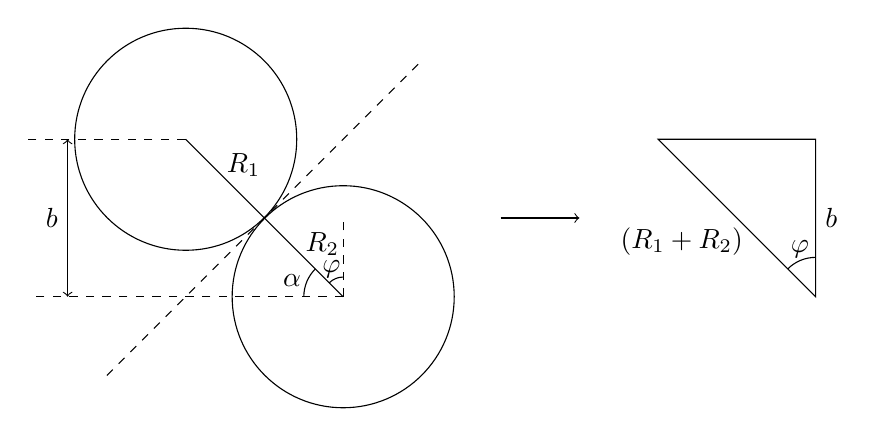
\begin{tikzpicture}
        %\draw[color=lightgray] (-1, -2) grid (10, 5);
        %\draw (0, 0) circle[radius=0.1];
        \draw (1, 2) circle[radius=1.41];
        \draw (3, 0) circle[radius=1.41];
        \draw[dashed] (0, -1) -- (4, 3);
        \draw (1, 2) -- (3, 0);
        \draw[dashed] (1, 2) -- (-1, 2);
        \draw[dashed] (3, 0) -- (-1, 0);
        \draw[<->] (-0.5, 0) -- (-0.5, 2);
        \node[left] at (-0.5, 1) {\(b\)};
        \node[above right] at (2.4, 0.4) {\(R_2\)};
        \node[above right] at (1.4, 1.4) {\(R_1\)};
        \begin{scope}
            \clip (3, 0) -- (2, 0) -- (2, 1) -- (3, 0);
            \draw (3, 0) circle[radius=0.5];
        \end{scope}
        \node at (2.35, 0.2) {\(\alpha\)};
        \begin{scope}
            \clip (3, 0) -- (2, 1) -- (3, 1) -- (3, 0);
            \draw (3, 0) circle[radius=0.25];
        \end{scope}
        \draw[dashed] (3, 0) -- (3, 1);
        \node at (2.85, 0.35) {\(\varphi\)};
        \draw[->] (5, 1) -- (6, 1);
        \draw (7, 2) -- (9, 2) -- (9, 0) -- cycle;
        \node[below left] at (8.2, 1) {\((R_1 + R_2)\)};
        \node[right] at (9, 1) {\(b\)};
        \begin{scope}
            \clip (7, 2) -- (9, 2) -- (9, 0) -- cycle;
            \draw (9, 0) circle[radius=0.5];
        \end{scope}
        \node at (8.8, 0.6) {\(\varphi\)};
        \end{tikzpicture}
        \caption{Collision between two spheres}
        \label{fig:collision between spheres}
    \end{figure}
    Figure \ref{fig:collision between spheres} shows the two spheres at the moment of contact.
    The angle \(\varphi = \pi/2 - \alpha\) and we have seen previously that \(\vartheta = \pi - 2\alpha\) so \(\varphi = \vartheta/2\).
    Using basic trig we get that
    \[b = (R_1 + R_2)\cos(\varphi) = (R_1 + R_2)\cos\left(\frac{\pi}{2} - \alpha\right) = (R_1 + R_2)\cos\left(\frac{\vartheta}{2}\right)\]
    The differential cross section is then
    \begin{align*}
        \sigma(\vartheta) &= -\frac{b}{\sin\vartheta}\dv{b}{\vartheta}\\
        &= -\frac{(R_1 + R_2)\cos\left(\!\frac{\vartheta}{2}\!\right)}{\sin\vartheta}\dv{\vartheta}\left[(R_1 + R_2)\cos\left(\frac{\vartheta}{2}\right)\right]\\
        &= -\frac{(R_1 + R_2)\cos\left(\!\frac{\vartheta}{2}\!\right)}{\sin\vartheta}\left[-\frac{1}{2}(R_1 + R_2)\sin\left(\frac{\vartheta}{2}\right)\right]\\
        &= \frac{(R_1 + R_2)^2\cos\left(\!\frac{\vartheta}{2}\!\right)\sin\left(\!\frac{\vartheta}{2}\!\right)}{2\sin\vartheta}\\
        &= \frac{(R_1 + R_2)^2\frac{1}{2}\sin\vartheta}{2\sin\vartheta}\\
        &= \frac{1}{4}(R_1 + R_2)^2
    \end{align*}
    Thus the total cross section is
    \[\sigma_T = 2\pi\frac{1}{4}(R_1 + R_2)^2\int_0^\pi \sin\vartheta\,\dd\vartheta = \pi(R_1 + R_2)^2\]
    which is the same as the result we got by inspection in section \ref{sec:diff cross sec}.
    The question that we now ask is what if we allow the second ball to move as in a game of pool?
    We now need to know the masses of the balls, we will take them to be \(m_1\) and \(m_2\).
    It is now useful to work in a different frame to answer the question.
    We work in the centre of mass (CM) frame as opposed to the LAB frame we were in previously.
    In the CM frame we define the origin to be where the centre of mass of the two balls is.
    We will denote quantities in the CM frame with a \(^*\) such as \(\vv v_1^*\), the velocity of ball one in the CM frame.
    In the CM frame both balls have equal and opposite momentums so ball one has momentum \(\vv p^*\) and ball two has momentum \(-\vv p^*\).
    The scattering angle is \(\vartheta^*\).
    The positions of the two balls in the CM frame are
    \[\vv r_1^* = \frac{\mu}{m_1}\vv r,\qquad \vv r_2^* = -\frac{\mu}{m_2}\vv r\]
    where \(\vv r = \vv r_1 - \vv r_2 = \vv r^*\) is the vector from ball two to ball one, and is the same in both frames, and \(\mu\) is the reduced mass defined as
    \[\mu = \frac{m_1 m_2}{m_1 + m_2}\]
    The velocities of the two balls are
    \[\vv v_1^* = \frac{\mu}{m_1}\dv{\vv r}{t} = \frac{\mu}{m_1}\vv v,\qquad \vv v_2^* = -\frac{\mu}{m_2}\dv{\vv r}{t} = -\frac{\mu}{m_2}\vv v\]
    where \(\vv v = \dd \vv r/\dd t\).
    The initial momenta in the LAB frame are 
    \[\vv p_1 = m_1\vv v_1,\qquad \vv p_2 = 0\]
    In the CM frame
    \[\vv p^* = m_1\vv v_1^* = -m_2\vv v_2^* = \mu\vv v = \mu\vv v_1\]
    since initially \(\vv v_2 = 0\) so \(\vv v = \vv v_1 - \vv v_2 = \vv v_1\).
    The velocity between the frames is
    \[\vv u = \frac{m_1\vv v_1}{m_1 + m_2} = \frac{\mu\vv v_1}{m_2} = \frac{\vv p^*}{m_2} = -\vv v_2^*\]
    In the CM frame both balls see a collision with a stationary object.
    The scattering angle is \(\vartheta^* = \pi - 2\alpha^*\) and the impact parameter is \(b = (R_1 + R_2)\cos(\vartheta^*/2)\) as for a stationary object, giving a differential cross section of \((R_1 + R_2)^2/4\) and a total cross section of \(\pi(R_1 + R_2)^2\).
    We now need to ask: What is \(\vartheta^*\) and how does it relate to values in the LAB frame that we can measure?
    
    \section{Rutherford Scattering}
    \subsection{Scattering angles in the CM and LAB frames}
    Since all motion in both frames is only along the \(x\) axis initially the \(y\) components of the CM and LAB frames are the same.
    If ball one scatters with a momentum \(\vv p_1\) at an angle \(\vartheta_1\) above the \(x\) axis then we can use the components of the momentum to find the angle as
    \[\tan(\vartheta_1) = \frac{p_1^y}{p_1^y}\]
    Using the fact that the \(y\) components are the same between frames we get
    \[p_1^y = m_1v_1^*\sin\vartheta^*\]
    Then using the fact that \(\vv v_1 = \vv v_1^* + m_1\vv u\) and the fact that \(u = m_1v_1^*/m_2\) we get
    \[p_1^x = m_1v_1^*\cos\vartheta^* + mu = m_1v_1^*\cos\vartheta^* + m_1\frac{m_1v_1^*}{m_2}\]
    So the angle is
    \[\tan(\vartheta_1) = \frac{m_1v_1^*\sin\vartheta^*}{m_1v_1^*\cos\vartheta^* + m_1\frac{m_1v_1^*}{m_2}} = \frac{\sin\vartheta^*}{\cos\vartheta^* + \frac{m_1}{m_2}}\]
    Given \(b\) we can calculate \(\vartheta^*\) from \(b = (R_1 + R_2)\cos(\vartheta^*/2)\).
    We can also calculate the angle \(\vartheta_2\) at which the second ball rebounds below the \(x\) axis using the same method.
    \[p_2^y = -m_2v_2^*\sin\vartheta^*\]
    \[p_2^x = m_2v_2^*\cos\vartheta^* - m_2v_2^*\]
    \[\tan(\vartheta_2) = \frac{p_2^y}{p_2^x} = \frac{-m_2v_2^*\sin\vartheta^*}{m_2v_2^*\cos\vartheta^* - m_2v_2} = \frac{\sin\vartheta^*}{1 - \cos\vartheta^*}\]
    This is independent of the masses.
    We now consider the case where \(m_1 = m_2\), we get
    \[\tan(\vartheta_1) = \frac{\sin\vartheta^*}{\cos\vartheta^* + 1} = \frac{2\cos\left(\!\frac{\vartheta^*}{2}\!\right)\sin\left(\!\frac{\vartheta^*}{2}\!\right)}{1 + 2\cos^2\left(\!\frac{\vartheta^*}{2}\!\right) - 1} = \frac{2\cos\left(\!\frac{\vartheta^*}{2}\!\right)\sin\left(\!\frac{\vartheta^*}{2}\!\right)}{2\cos^2\left(\!\frac{\vartheta^*}{2}\!\right)} = \frac{\sin\left(\!\frac{\vartheta^*}{2}\!\right)}{\cos\left(\!\frac{\vartheta^*}{2}\!\right)} = \tan\left(\frac{\vartheta^*}{2}\right)\]
    so \(\vartheta_1 = \vartheta^*/2\) since all angles are in \([0, \pi]\).
    Doing the same with  \(\vartheta_2\) we get
    \[\tan(\vartheta_2) = \frac{\sin\vartheta^*}{1 - \cos\vartheta^*} = \frac{2\cos\left(\!\frac{\vartheta^*}{2}\!\right)\sin\left(\!\frac{\vartheta^*}{2}\!\right)}{1 - 2\cos^2\left(\!\frac{\vartheta^*}{2}\!\right) + 1} = \frac{2\cos\left(\!\frac{\vartheta^*}{2}\!\right)\sin\left(\!\frac{\vartheta^*}{2}\!\right)}{2 - 2\cos^2\left(\!\frac{\vartheta^*}{2}\!\right)} = \frac{\cos\left(\!\frac{\vartheta^*}{2}\!\right)\sin\left(\!\frac{\vartheta^*}{2}\!\right)}{1 - \cos^2\left(\!\frac{\vartheta^*}{2}\!\right)}\] 
    \[= \frac{\cos\left(\!\frac{\vartheta^*}{2}\!\right)\sin\left(\!\frac{\vartheta^*}{2}\!\right)}{\sin^2\left(\!\frac{\vartheta^*}{2}\!\right)} = \frac{\cos\left(\!\frac{\vartheta^*}{2}\!\right)}{\sin\left(\!\frac{\vartheta^*}{2}\!\right)} = \frac{\sin\left(\!\frac{\pi}{2} - \frac{\vartheta^*}{2}\!\right)}{\cos\left(\!\frac{\pi}{2} - \frac{\vartheta^*}{2}\!\right)} = \tan\left(\frac{\pi}{2} - \frac{\vartheta^*}{2}\right)\]
    so \(\vartheta_2 = \pi/2 - \vartheta^*/2\).
    The balls recoil from each other at an angle of \(\vartheta_1 + \vartheta_2 = \vartheta^*/2 +\pi/2 - \vartheta^*/2 = \pi/2\) so the balls recoil at a right angle.
    
    \subsection{Rutherford Scattering}
    In Rutherford's famous scattering experiment he and his collaborators, Hans Geiger and Ernest Marsden, fired alpha particles at a gold foil and measured the angle at which they were deflected.
    Based on the plumb pudding model of the atom they expected the alpha particles to be deflected very little so were very surprised when a significant number of alpha particles were deflected at large angles.
    This could only be explained if there was a large concentration of charge in one place.
    This turned out to be key information for the existence of the nucleus.
    We now know that this charge concentration is positive but the same maths would hold if it were negative.
    
    The question that we now want to answer is what is the size of the nucleus?
    Alpha particles were fired at the gold foil with impact parameter \(b\).
    The angle \(\alpha = \pi/2 - \vartheta/2\) is such that
    \[\tan\alpha = \frac{b}{a} \implies b = a\cot\frac{\vartheta}{2}\]
    For hyperbolic orbits the energy is
    \[E = \frac{k}{2a}\implies a = \frac{k}{2E}\implies b = \frac{k}{2E}\cot\frac{\vartheta}{2}\]
    For the case of Rutherford scattering the force is the Coulomb force so \(k = qQ/(4\pi\varepsilon_0)\).
    \[\dv{b}{\vartheta} = -\frac{k}{4E}\cosec^2\frac{\vartheta}{2}\]
    \[\sigma(\vartheta) = -\frac{b}{\sin\vartheta}\dv{b}{\vartheta} = \frac{k^2}{16E^2\sin^4\frac{\vartheta}{2}}\]
    If we put in the constants and find \(k\) for the case of an alpha particle and gold nucleus then we get
    \[\sigma(\vartheta) = \frac{\SI{0.766e-28}{m^2}}{\sin^4\frac{\vartheta}{2}}\]
    We define the unit \(\SI{1}{barn} = \SI{e-28}{m^2}\) for use with this sort of calculation.
    When making measurements Rutherford predicted this and the results confirmed it.
    For small values of \(\vartheta\) \(\sigma\) is very big however \(\sigma\) is small compared to the size of the atom and the nucleus is smaller than \(\sigma\) since the repulsive force acts at a distance so the nucleus must be very small.
    
    \subsection{Rutherford Scattering by Momentum Change}
    It is also possible to answer the same question using the change of momentum.
    If the total momentum is \(\vv p\) then the change in momentum after deflection is \(|\Delta\vv p| = 2p\cos\alpha\).
    Since the \(y\) component of momentum is unchanged by the deflection and the \(x\) component starts at \(-p\cos\alpha\) and ends at \(p\cos\alpha\).
    In time \(\dd t\) the force is
    \[F_x = \frac{k}{r^2}\cos\vartheta'\]
    where \(\vartheta'\) is the polar coordinate.
    The momentum change is
    \[|\Delta\vv p| = \int_{-\infty}^\infty \frac{k}{r^2}\cos\vartheta'\,\dd t = 2p\cos\alpha\]
    \[\omega = \dv{\vartheta'}{t} = \frac{L}{mr^2} = \frac{mv_\infty b}{mr^2} = \frac{v_\infty b}{r^2} \implies \frac{1}{r^2}\dd t = \frac{1}{v_\infty b}\dd\vartheta'\]
    \[|\Delta\vv p| = \int_{-\alpha}^\alpha \frac{k\cos\vartheta'}{v_\infty b}\,\dd\vartheta ' = \frac{k}{v_\infty b}\int_{-\alpha}^\alpha \cos\vartheta' \,\dd\vartheta' = \frac{2k\sin\alpha}{bv_\infty}\]
    \[b = \frac{2k\sin\alpha}{v_\infty|\Delta\vv p|} = \frac{2k\sin\alpha}{v_\infty2p\cos\alpha} = \frac{k}{pv_\infty}\tan\alpha = \frac{k}{mv_\infty^2}\tan\alpha = \frac{k}{2E}\tan\alpha = \frac{k}{2E}\cot\frac{\vartheta}{2}\]
    using \(p = mv_\infty\) and \(E = mv_\infty^2/2\).
    This gives the same value of \(b\) as the previous method so will result in the same prediction for the cross section of the nucleus.
    
    \section{Non--inertial Frames}
    A frame \(S'\) is accelerating in frame S at constant acceleration \(\vv A\).
    An object with acceleration \(\vv a\) in frame S will have acceleration \(\vv a' = \vv a - \vv A\) in frame \(S'\).
    The object will then have a velocity
    \[\vv v' = \int \vv a - \vv A\,\dd t = \vv v + \vv u - \vv At\]
    where the constant of integration \(\vv u = \vv v'(0) - \vv v(0)\) is the velocity of frame \(S'\) in frame \(S\) at \(t = 0\).
    In frame \(S'\) the object sees a fictitious force \(\vv F' = -m\vv A\) to explain the motion.
    Alternatively in frame \(S\) an object at rest in frame \(S'\) has a real force \(\vv F = m\vv A\) being applied to it.
    
    \subsection{Rotating Frame}
    \(S\) is a fixed frame such as the fixed stars frame and \(S'\) is a rotating frame such as Earth.
    We want to know how a vector transforms from frame \(S\) to \(S'\) and vice versa.
    We consider an arbitrary vector \(\vv B\) in frame \(S\).
    To define \(\vv B\) in each frame we need a set of basis vectors.
    In frame \(S\) we use \(\{\vi, \vj, \vk\}\) and in frame \(S'\) we choose \(\{\vi', \vj', \vk'\}\).
    Hence in the two frames \(\vv B\) is:
    \[\vv B = B_x\vi + B_y\vj + B_z\vk\]
    \[\vv B = B_x'\vi' + V_y'\vj' + B_z'\vk'\]
    Note that this is the same vector in both frames, we are dealing with passive transforms between frames.
    We consider the time derivatives of \(\vv B\) in each frame:
    \[\left[\dv{\vv B}{t}\right]_S = \dv{B_x}{t}\vi + \dv{B_y}{t}\vj + \dv{B_z}{t}\vk\]
    \[\left[\dv{\vv B}{t}\right]_{S'} = \dv{B_x'}{t}\vi + \dv{B_y'}{t}\vj + \dv{B_z'}{t}\vk + B_x'\dv{\vi'}{t} + B_y'\dv{\vj'}{t} + B_z'\dv{\vk'}{t}\]
    The first three terms are just \(\dd\vv B'/\dd t\).
    The last three terms are there as the basis vectors in frame \(S'\) are not constant in time.
    Consider the small change \(\dd\vi'\) in time \(\dd t\).
    It is possible to show geometrically that
    \[\left|\dv{\vi'}{t}\right| = \dv{\vartheta}{t} = \omega\]
    and that the direction is given by
    \[\dv{\vi'}{t} = \vv\omega\times\vi'\]
    The same can be done for \(\vj'\) and \(\vk'\).
    Hence we can relate the derivatives as
    \[\left[\dv{\vv B}{t}\right]_S = \left[\dv{\vv B'}{t}\right] + \vv\omega\times\vv B\]
    
    \subsection{Fictitious Forces}
    If we set \(\vv B = \vv r\) then we get
    \[\vv v_S = \left[\dv{\vv r}{t}\right]_S\]
    \[\vv v_S = \vv v_{S'} + \vv\omega\times\vv r\]
    Since we are only dealing with rotations \(\vv r\) doesn't depend on the frame so \(\vv r' = \vv r\).
    Now we set \(\vv B = \vv v_S\) and we get
    \[\vv a_S = \left[\dv{\vv v}{t}\right]_S\]
    \[\vv a_S = \vv a_{S'} + \vv\omega\times\vv v_S = \vv a_{S'} + \vv\omega\times(\vv v_{S'} + \vv\omega\times\vv r) = \vv a_{S'} + \vv\omega\times\vv v_{S'} + \vv\omega\times(\vv\omega\times\vv r)\]
    \[\vv a_{S'} = \left[\dv{\vv v_S}{t}\right]_{S'} = \dv{t}[\vv v_{S'} + \vv\omega\times\vv r] = \dv{\vv v_{S'}}{t} + \vv\omega\times\vv v_{S'}\]
    where we have used the fact that \(\vv\omega\) is a constant and that \(\dd\vv r/\dd t = \vv v_{S'}\).
    Combining these
    \[\vv a_S = \vv a_{S'} + 2\vv\omega\times\vv v_{S'} + \vv\omega\times(\vv\omega\times\vv r)\]
    Rearranging this and multiplying through by the mass we get
    \[\vv F_{S'} = \vv F_S - 2m\vv\omega\times\vv v_{S'} - m\vv\omega\times(\vv\omega\times\vv r)\]
    The second term, \(2m\vv\omega\times\vv v_{S'}\), is the Coriolis force and the last term, \(m\vv\omega\times(\vv\omega\times\vv r)\), is the centrifugal force.
    Both are fictitious forces that are needed in the, non--inertial, rotating frame to explain motion.
    Note that the magnitude of the Coriolis force is proportional to \(\omega\) whereas the magnitude of the centrifugal force is proportional to \(\omega^2\).
    This means that for small \(\omega\ll 1\) it is often possible to ignore the centrifugal force as it is a much smaller effect than the Coriolis force.
    For large values of \(\omega\) the opposite is true.
    
    \subsection{Earth As a Rotating Frame}
    The Earth is a rotating frame with the fixed (far away) stars as an inertial frame.
    The angular velocity of Earth is
    \[\vv\omega_E = \frac{2\pi}{24\cdot60\cdot60}\vk = \SI{7.3e-5}{rad.s^{-1}}\vk\]
    Where \(\vk\) is defined as being the axis of rotation.
    This is a very small value so for most cases we don't need to consider it.
    Even when it is important it is often possible to ignore the centrifugal force as it is proportional to \(\omega_E^2 = \SI{5.3e-9}{rad^2.s^{-2}}\).
    
    \example
    A skydiver jumps from a stationary object such that they have no horizontal velocity relative to Earth.
    They start directly above a target.
    We define the coordinate system on Earth as \(x'\) being North, \(y'\) being East and \(z'\) being height above the surface of Earth.
    We can see immediately that \(x' = x\) since all motion of Earth is along the \(y'\) direction.
    We will ignore the centrifugal force.
    Newton's second law gives us
    \[m\dv[2]{y'}{t}\vj' = -2m\vv\omega_E\times\vv v_{S'}\]
    We need to find the \(\vj'\) component of the cross product:
    \[(\vv\omega_E\times\vv v_{S'})\cdot\vj' = \omega_{x'}v_{z'} - \omega_{z'}v_{x'}\]
    \(v_{x'} = 0\) since there is no horizontal motion in the Earth frame.
    It is possible to show that at a latitude \(\varphi\) the angular frequency has \(x'\) component \(\omega_{x'} = \omega_E\cos\varphi\).
    \[(\vv\omega_E\times\vv v_{S'})\cdot\vj' = \omega_E\cos(\varphi)\dv{z'}{t}\]
    \[\dv[2]{y'}{t} = -2\omega_E\cos(\varphi)\dv{z'}{t} = 2\omega_E gt\cos(\varphi)\]
    Where we used the fact that \(\ddot z' = -g\implies \dot z = -gt\) where the constant of integration is zero as at \(t = 0\) the downward velocity is zero.
    \[y' = \frac{1}{3}\omega_Egt^3\cos\varphi\]
    This is how far they will be from the target when they hit the ground.
    
    \subsection{Foucault's Pendulum}
    Foucault's pendulum is an experiment where a large (so it keeps swinging for a long time) pendulum is swung and as Earth spins the Coriolis force cause the plane through which the pendulum swings to rotate relative to Earth.
    The set up to calculate how much is the same as in section \ref{sec:pendulum} but we now include the Coriolis force as well.
    Newton's second law gives
    \[m\left[\dv{\vv v'}{t} + 2\vv\omega_E\times\vv v'\right] = -mg\vh z' - T\vh r'\]
    where \(\vh z'\) is the distance of the pendulum above the lowest point of its swing and \(\vh r'\) is a unit vector from the point where it is attached towards the bob and \(T\) is the tension.
    The cross product gives us
    \[\vv\omega_E\times\vv v' = (\omega_{y'}v_{z'} - \omega_{z'}v_{y'})\vi' + (\omega_{z'}v_{x'} - \omega_{x'}v_{z'})\vj' + (\omega_{x'}v_{y'} - \omega_{y'}v_{x'})\vk'\]
    Vertical displacements are small so we can approximate \(v_z = 0\) and the \(\vk'\) component is unimportant so we discard it.
    This leaves us with
    \[\vv\omega_E\times\vv v' = -\omega_{z'}v_{y'}\vi' + \omega_{z'}v_{x'}\vj'\]
    As before we can show \(\omega_{z'} = \omega_E\sin\varphi\) so we have
    \[\vv\omega_E\times\vv v' =\omega_E\sin(\varphi)\dv{y'}{t}\vi' + \omega_E\sin(\varphi)\dv{x'}{t}\vj'\]
    We can put this into the original Newton's second law equation and split it into two components
    \[\dv[2]{x'}{t} - 2\omega_E\sin(\varphi)\dv{y'}{t} + \omega_0^2x' = 0\]
    \[\dv[2]{y'}{t} + 2\omega_E\sin(\varphi)\dv{x'}{t} + \omega_0^2y' = 0\]
    where \(\omega_0 = \sqrt{g/L}\).
    We make the ansatz that \(x' = \cos(\alpha t)\) and \(y' = \sin(\alpha t)\) are solutions and substituting in to the \(x'\) equation we get
    \[-\alpha^2\cos(\alpha t) - 2\omega_E\alpha\sin(\varphi)\cos(\alpha t) + \omega_0^2\cos(\alpha t) = 0\]
    \[-\alpha^2 - 2\omega_E\sin(\varphi) + \omega_0 = 0\]
    \[\alpha = \frac{2\omega_E\sin(\varphi) \pm \sqrt{[2\omega_E\sin(\varphi)]^2 + 4\omega_0^2}}{-2}\]
    \[\alpha = -\omega_E\sin(\varphi) \pm \sqrt{[\omega_E\sin(\varphi)]^2 + \omega_0^2}\]
    \(\alpha\) is the frequency at which the pendulum precesses.
    In Edinburgh \(\varphi = \SI{56}{\SIUnitSymbolDegree}\) and the rate of rotation is \(\SI{298}{\SIUnitSymbolDegree}\) per day.
    
    \section{Rigid Bodies}
    So far we have treated all objects as point masses but in reality all objects have size.
    We will consider rigid bodies that maintain their shape and size.
    The best way to describe a rigid body for dynamics is using its moment of inertia, which in the most general case is a 2--tensor.
    We can consider the moments of inertia, \(I\), about the principle symmetry axes of the body.
    This introduces three additional degrees of freedom for rotation about the three principle symmetry axes.
    These are orthogonal and pass through the centre of mass of the body.
    
    \subsection{Moments of Inertia}
    The moment of inertia of a rigid body about one of its principle axes \(A\) is
    \[I_A = \int_V|\vv r_A|^2\rho(\vv r)\,\dd V\]
    where \(V\) is the volume of the body, \(\vv r_A\) is the distance of \(\vv r\) perpendicular to the axes \(A\) and \(\rho(\vv r)\) is the mass density of the object.
    To simplify things we will restrict ourselves to uniform densities and simple shapes.
    Some common moments of inertia are
    \begin{itemize}
        \item A hoop of radius \(R\) and mass \(M\) about the symmetry axis through its centre.
        Here \(|\vv r_A| = R\) so
        \[I = R^2\int\rho\,\dd V = MR^2\]
        Note that this doesn't require constant \(\rho\) since this is the definition of \(\rho\).
        
        \item A solid cylinder of radius \(R\), height \(H\), and mass \(M\) about its symmetry axis
        \[I = H\rho\int_0^Rr^2_A2\pi r_A\,\dd r_A = 2\pi H\rho\frac{R^4}{4}\]
        The volume \(V\) is
        \[V = \int_0^R2\pi r_A\,\dd r_A = 2\pi H\frac{R^2}{2}\]
        so this is
        \[I = \frac{1}{2}\rho VR^2 = \frac{1}{2}MR^2\]
        
        \item A solid sphere (ball) of radius \(R\) and mass \(M\) about an axis through its centre
        \[I = \frac{2}{5}MR^2\]
        
        \item A spherical shell (sphere) of radius \(R\) and mass \(M\) about an axis through its centre
        \[I = \frac{2}{3}MR^2\]
        
        \item A thin rod of length \(L\) and mass \(M\) about its centre
        \[I = \frac{1}{12}ML^2\]
    \end{itemize}
    The numerical factor in each of these can be absorbed into the definition of the radius of gyration, \(k_A\), for each object:
    \[k_A^2 = \frac{1}{M}\int |\vv r_A|^2\rho(\vv r)\,\dd V\]
    \[I_A = Mk_A^2\]
    This represents the distance from the axis where the mass would need to be put in a hoop to give the same moment of inertia.
    
    \subsection{Parallel and Perpendicular Axes}
    The parallel axes theorem states that for parallel axis \(A\) and \(A'\) with a distance \(d\) between axes if \(A\) passes through the centre of mass then we can find \(I_{A'}\) as
    \[I_{A'} = I_A + Md^2\]
    This can be proved by replacing \(\vv r_A\) with \(\vv r_A + \vv d\) in the definition of \(I_A\) and recognising that by the definition of the centre of mass
    \[\int\vv r_A\rho\,\dd V = \vv 0\]
    since \(A\) passes through the centre of mass so \(\vv r_A = \vv 0\).
    
    The perpendicular axes theorem states that if instead \(A'\) is perpendicular to \(A\) then
    \[I = I_A + I_{A'}\]
    This can be shown by setting \(\vv r_A\) to \(\vv r_A + \vv d\) and using the fact that \(\vv r_A\cdot\vv d = 0\).
    
    From this we can deduce that:
    \begin{itemize}
        \item A hoop has a moment of inertia about an axis through its centre and in the plane of the hoop of
        \[I = \frac{1}{2}MR^2\]
        \item A cylinder has a moment of inertia about an axis through its centre, perpendicular to the symmetry axis, of
        \[I = \frac{1}{4}MR^2 + \frac{1}{12}MH^2\]
    \end{itemize}
    
    \subsection{The Inertia Tensor}
    For more complicated and non--uniform shapes the moments of inertia can be generalised in the form of the moment of inertia tensor:
    \[I_{ij} = \int\left[\delta_{ij}\left(\sum_{k=1}^3 x_k^2\right) - x_ix_j\right]\rho\,\dd V\]
    The moments of inertia for the three Cartesian axes are the diagonal of this tensor.
    \[I_{11} = I_x = \int(y^2 + z^2)\rho\,\dd V,\qquad I_{22} = I_y = \int(x^2 + z^2)\rho\,\dd V,\qquad I_{33} = I_z = \int(x^2 + y^2)\rho\,\dd V\]
    The off diagonal elements are
    \[I_{12} = I_{21} = -\int(xy)\rho\,\dd V,\qquad I_{23} = I_{32} = -\int(yz)\rho\,\dd V,\qquad I_{31} = I_{13} = -\int(xz)\rho\,\dd V\]
    The inertia tensor is a symmetric matrix that can be diagonalised by finding the eigenvalues and eigenvectors and constructing the transformation matrix \(\mat M\) such that the diagonalised moment of inertia tensor \(\mat I'\) is
    \[\mat I' = \mat M\cdot\mat I\cdot\mat M\trans\]
    If this is done then you will find that \(\mat M\) represents a rotation from the Cartesian coordinates to the principle axes of the body.
    
    \subsection{Rolling}
    An object being a rigid body is important only if there is rotation about an axis since if it doesn't rotate the physics is the same as for a point mass.
    The angular momentum of a body around an axis, \(A\), is
    \[L = I_A\omega_A\]
    where \(\vv L\) and \(\vv \omega_A\) point along the direction of \(A\).
    The rotational kinetic energy is
    \[T = \frac{1}{2}I_A\omega_A^2\]
    This can be written more generally with the inertia tensor as
    \[\vv L = \mat I\cdot\vv\omega,\qquad L_i = I_{ij}\omega_j\]
    \[T = \frac{1}{2}\vv\omega\trans\cdot\mat I\cdot\vv\omega\]
    Spherical or cylindrical objects will roll across a surface.
    For an object of radius \(R\) in order to be rolling with no sliding the distance travelled during rotation \(\Delta\vartheta\) must be \(\Delta x = R\Delta\vartheta\).
    Dividing by \(\Delta t\) we get
    \[v = \frac{\Delta x}{\Delta t} = R\frac{\Delta\vartheta}{t} = R\omega\]
    More generally the roll condition is
    \[\vv v = R(\vv\omega\times\vk)\]
    where \(\vk\) is normal to the surface.
    Hence to roll without sliding the object must satisfy two equations, one for linear velocity, set by the force, and one for angular velocity, set by the torque.
    If it doesn't then the object will slide as well as roll.
    
    \example
    Consider a pool ball at rest on a table.
    If it is struck by a cue through its centre then initially there is a force but no torque.
    The roll condition can't be satisfied immediately because \(\vv\omega\) is zero but \(\vv v\) isn't.
    If you want immediate rolling the ball needs to be struck with impact parameter \(b\) above its centre such that the force and torque are just right to satisfy the rolling condition.
    What is \(b\)?
    
    The linear force is
    \[F = M\dv{v}{t} = MR\dv{\omega}{t}\]
    using the roll condition that \(v = R\omega\).
    Meanwhile the torque is \(\tau = |\vv r\times\vv F|\).
    This picks out the perpendicular distance at which the force is applied relative to the centre of the ball which we have defined as \(b\).
    Hence 
    \[\tau = bF = bMR\dv{\omega}{t}\]
    We can equate this to the torque
    \[\tau = I\dv{\omega}{t},\qquad I = \frac{2}{5}MR^2\]
    \[bMR\dv{\omega}{t} = I\dv{\omega}{t} = \frac{2}{5}MR^2\dv{\omega}{t}\implies b = \frac{2}{5}R\]
    Hence the ball must be struck at a distance \(0.4R\) above the centre to roll initially.
    Using the different moments of inertia we can show that for hollow sphere \(b = 2R/3\) and for a cylinder \(b = 0.5 R\).
    
    \example
    Now the pool table has friction.
    The ball is struck in the middle.
    At first it slides and there is only translational motion.
    Friction will cause the ball to slow down and will also apply a torque to the ball, at some point the roll condition will be satisfied and the ball will start rolling.
    At what velocity relative to the initial velocity \(V\) does this happen?
    
    We assume that until the roll condition is satisfied the ball's motion is purely translational.
    After the ball starts moving it experiences a force \(\vv F = -F_\text{frict}\vi\).
    The linear force is equation is thus
    \[M\dv{\vv v}{t} = -F_\text{frict}\vi\]
    As before we substitute this into the equation for torque.
    The frictional force is applied along the surface of the ball so at a point \(\vv r = -R\vk\) where the ball meets the table.
    Hence
    \[\tau = \frac{2}{5}MR^2\dv{\vv\omega}{t} = \vv r\times\vv F = (-R\vk)\times(-F_\text{frict}\vi) = (-R\vk)\times \left(M\dv{\vv v}{t}\right)\]
    \[\frac{2}{5}MR^2\dv{\vv\omega}{t} = -MR\left(\vk\times\dv{\vv v}{t}\right)\]
    Now we want to apply the roll condition.
    First we think about the directions of things.
    The velocity is in the \(x\) direction so \(\vv v = v_x\vi i\).
    The rotation is in the \(y\) direction so \(\vv\omega = \omega_y\vj\). 
    Since \(\vk\times\vi = \vj\) the result for both sides is in the \(\vj\) direction which is good.
    Substituting for \(\vv v\) and \(\vv\omega\) we get
    \[\dv{v_x}{t} = -\frac{2}{5}R\dv{\omega_y}{t}\]
    Integrating with respect to time and noting that the initial \(x\) velocity is \(V\) and there is no initial rotation we get
    \[\int_0^t\dv{v_x}{t}\,\dd t = v_x(t) - v_x(0) = v_x(t) - V = -\frac{2}{5}R\int_0^t \dv{\omega_y}{t}\,\dd t = -\frac{2}{5}R[\omega_y(t) - \omega_y(0)] = -\frac{2}{5}R\omega_y(t)\]
    \[v_x(t) - V = \frac{2}{5}R\omega_y(t)\]
    For the roll condition to be satisfied we need \(v_x = R\omega_y\).
    Solving for \(v_x\) we get
    \[v_x(\tau) - V = \frac{2}{5}v_x(\tau)\implies v_x(\tau) = \frac{5}{7}V\]
    where \(\tau\) is the time when rolling starts.
    So if the ball is hit in the middle it loses \(2/7\) of its initial speed before it starts to roll.
    Notice that this is independent of \(F_\text{frict}\) or the radius.
    
    \section{Lagrangian Dynamics}
    Lagrangian dynamics is another way to get the the equations of motion.
    Previously we have used Newton's second law, conservation of energy and conservation of momentum.
    We still need to solve the equations of motion after we find them but that is ``just maths".
    
    \subsection{The Euler--Lagrange Equation}
    Given a function \(f\) of variables \(q\) and \(\dot q = \partial_t q\) the principle of least action states that \(f\) is such that the action, \(S\), is minimised (or strictly speaking extremised).
    The action is defined as
    \[S = \int_{t_1}^{t_2}f(q, \dot q)\,\dd t\]
    Here we are working only in one dimension (\(q\) and \(\dot q\)).
    All of the maths holds for \(n\) dimensions if the coordinates \(q_i\) where \(i = 1,\dotsc,n\) are independent of each other and as such any cross terms in derivatives are zero.
    It is just a lot more terms to write.
    
    What does it mean for \(f\) for it to satisfy the principle of least action?
    Both \(q\) and \(\dot q\) are functions of \(t\) so depend on the path taken from \(t_1\) to \(t_2\).
    Define the ``true" path taken from \(t_1\) to \(t_2\) to be the one that minimises \(S\).
    This path can be parametrised as \(q_\text{true}(t)\).
    Any other path from \(t_1\) to \(t_2\) can then be described by how it differs from this path.
    We define the deviation \(\eta(t)\) to be a function for a path \(q(t)\) such that
    \begin{equation}\label{eqn:q}
        q(t) = q_\text{true}(t) + \varepsilon\eta(t)
    \end{equation}
    where \(\varepsilon\) is some small constant independent of \(t\).
    This gives
    \begin{equation}\label{eqn:q dot}
        \dot q(t) = \dot q_\text{true}(t) + \varepsilon \dv{\eta}{t}
    \end{equation}
    Mathematically what it means to minimise \(S\) is to have
    \[\dv{S}{\varepsilon} = 0\]
    We can find this value from the definition of \(S\) and use it to impose restrictions of \(f\):
    \[\dv{S}{\varepsilon} = \dv{\varepsilon}\int_{t_1}^{t_2} f(q, \dot q)\,\dd t\]
    Since \(\varepsilon\) and \(t\) are independent of each other we can bring the derivative into the integral and we get
    \[\dv{S}{\varepsilon} = \int_{t_1}^{t_2} \dv{f}{\varepsilon}\,\dd t\]
    We can then use the chain rule to express the integrand in terms of the derivatives of \(f\) with respect to \(q\) and \(\dot q\) and the derivatives of \(q\) and \(\dot q\) with respect to \(\varepsilon\):
    \[\dv{S}{\varepsilon} = \int_{t_1}^{t_2} \left(\pdv{f}{q}\dv{q}{\varepsilon} + \pdv{f}{\dot q}\dv{\dot q}{\varepsilon}\right) \,\dd t\]
    Differentiating equations \ref{eqn:q} and \ref{eqn:q dot} with respect to \(\varepsilon\) we get
    \[\dv{q}{\varepsilon} = \dv{\varepsilon}[q_\text{true}(t) + \varepsilon\eta(t)] = \eta(t)\]
    \[\dv{\dot q}{\varepsilon} = \dv{\varepsilon}\left[\dot q_\text{true}(t) + \varepsilon\dv{\eta}{t}\right] = \dv{\eta}{t}\]
    Substituting this back into our equation we get
    \[\dv{S}{\varepsilon} = \int_{t_1}^{t_2}\left(\pdv{f}{q}\eta + \pdv{f}{\dot q}\dv{\eta}{t}\right)\]
    The second term can be expressed as the derivative of a product:
    \[\dv{t}\left(\pdv{f}{\dot q}\eta\right) = \pdv{f}{\dot q}\dv{\eta}{t} + \dv{t}\left(\pdv{f}{\dot q}\right)\eta\]
    \[\implies \pdv{f}{\dot q}\dv{\eta}{t} = \dv{t}\left(\pdv{f}{\dot q}\eta\right) - \dv{t}\left(\pdv{f}{\dot q}\right)\eta\]
    Substituting into our original integral we get
    \[\dv{S}{\varepsilon} = \int_{t_1}^{t_2}\left[\pdv{f}{q}\eta + \dv{t}\left(\pdv{f}{\dot q}\eta\right) - \dv{t}\left(\pdv{f}{\dot q}\right)\eta\right] \,\dd t\]
    Using the linearity of the integral this is
    \[\dv{S}{\varepsilon} = \int_{t_1}^{t_2}\left[\pdv{f}{q}\eta - \dv{t}\left(\pdv{f}{\dot q}\right)\eta\right]\,\dd t + \int_{t_1}^{t_2} \dv{t}\left(\pdv{f}{\dot q}\eta\right)\,\dd t\]
    Using the fundamental theorem of calculus the second integral is
    \[\int_{t_1}^{t_2}\dv{t}\left(\pdv{f}{\dot q}\eta\right)\,\dd t = \left[\pdv{f}{\dot q}\eta(t)\right]_{t_1}^{t_2} = \pdv{f}{\dot q}\biggr|_{t = t_2}\eta(t_2) - \pdv{f}{\dot q}\biggr|_{t = t_1}\eta(t_1) = 0\]
    Since for the path to start and end in the same place we require that \(q(t_1) = q_\text{true}(t_1)\) and \(q(t_2) = q_\text{true}(t_2)\).
    This is true if and only if \(\eta(t_1) = \eta(t_2) = 0\) so the integral above is zero.
    Hence
    \[0 = \dv{S}{\varepsilon} = \int_{t_1}^{t_2}\left[\pdv{f}{q} - \dv{t}\left(\pdv{f}{\dot q}\right)\right]\eta\,\dd t\]
    For this to be true for we require the integrand to be zero and for non--zero \(\eta(t)\) this forces
    \[\pdv{f}{q} = \dv{t}\left(\pdv{f}{\dot q}\right)\]
    This is the Euler--Lagrange equation and is true for any \(f\) that satisfies the principle of least action.
    It can be extended to multiple dimensions for a function \(f\) of independent variables \(\{q_i\}\) and their derivatives \(\{\dot q_i\}\) the Euler--Lagrange equation becomes a series of equations
    \[\pdv{f}{q_i} = \dv{t}\left(\pdv{f}{\dot q_i}\right)\]
    Note that so far this is just maths.
    This holds for any function \(f\) that satisfies the principle of least action and any independent variables \(\{q_i\}\).
    Even \(t\) doesn't have to be time.
    To do physics though we want to give a physical meaning to all quantities and we do this using the Lagrangian.
    
    \subsection{The Lagrangian}
    Lagrange showed that there was a particular form of \(f\) that allowed for a lot of equations of motion to be found.
    The particular form he found that satisfies the principle of least action is now known as the Lagrangian:
    \[\LL(q_i, \dot q_i) = T - V\]
    where \(\{q_i\}\) are some generalised coordinates, \(\{\dot q_i\}\) are some generalised velocities and \(T\) and \(V\) are the kinetic and potential energies of the system at the coordinates.
    Generally the kinetic energy is a function of the velocities, \(T = T(\dot q_i)\) and the potential is a function of both position and velocity so \(V = V(q_i, \dot q_i)\).
    Since the Lagrangian satisfies the principle of least action we require that it satisfies the Euler--Lagrange equations
    \[\pdv{\LL}{q_i} = \dv{t}\left(\pdv{\LL}{\dot q_i}\right)\]
    
    \example
    Linear motion can be described in Lagrangian mechanics.
    The kinetic energy of a particle of mass \(m\) in Cartesian coordinates is
    \[T(v_x, v_y, v_z) = \frac{1}{2}m(v_x^2 + v_y^2 + v_z^2)\]
    We assume a potential that depends only on position so the Lagrangian of the system is
    \[\LL = \frac{1}{2}m(v_x^2 + v_y^2 + v_z^2) - V(x, y, z)\]
    Applying the Euler--Lagrange equations for the \(x\) coordinate we get
    \[\pdv{\LL}{x} = -\pdv{V}{x} = F_x\]
    \[\dv{t}\left(\pdv{\LL}{v_x}\right) = \dv{t}\left(mv_x\right) = ma_x\]
    \[\implies F_x = ma_x\]
    We can do the same for the \(y\) and \(z\) coordinates and we recover \(\vv F = m\vv a\) which is Newton's second law.
    
    \example
    Next we consider rotation around the \(z\) axis.
    This is most naturally described in plane polar coordinates \((r, \vartheta)\).
    Assuming a potential dependent only on position the Lagrangian is
    \[\LL = \frac{1}{2}m(r^2\omega^2 + v_r^2) - V(r, \vartheta)\]
    Note that \(v_r = \dot r\) and \(\omega = \dot\vartheta\).
    Applying the Euler--Lagrange equations for the \(r\) coordinate
    \[\pdv{\LL}{r} = mr\omega^2-\pdv{V}{r} = mr\omega^2 - F_r\]
    \[\dv{t}\left(\pdv{\LL}{v_r}\right) = \dv{t}[mv_r] = m\dv{v_r}{t}\]
    \[mr\omega^2 - F_r = m\dv{v_r}{t}\]
    \[F_r = m\dv{v_r}{t} - mr\omega^2\]
    This is Newton's second law with centripetal force \(mr\omega^2\).
    We can do the same for the \(\vartheta\) coordinate and we get
    \[\pdv{\LL}{\vartheta} = -\pdv{V}{\vartheta} = rF_\vartheta\]
    \[\dv{t}\left(\pdv{\LL}{\omega}\right) = \dv{t}[mr^2\omega] = mr^2\dv[2]{\vartheta}{t}\]
    \[rF_\vartheta = mr^2\dv{\omega}{t}\]
    The term on the left is is the torque \(\tau = |\vv r\times\vv F|\) and the term on the right is the moment of inertia times the time derivative of \(\vartheta\) so we have recovered the rotational analogue of Newton's second law:
    \[\vv\tau = I\dv{\vv\omega}{t}\]
    
    \example
    We can use Lagrangian mechanics to find the equations of motion for a pendulum.
    If the length of the pendulum is \(L\) and the mass of the bob is \(m\) then the kinetic energy is
    \[T = \frac{1}{2}mL^2\omega^2\]
    The potential energy is the gravitational potential.
    A little bit of geometry tells us that if the pendulum is at an angle \(\vartheta\) to the vertical then the bob is \(L(1 - \cos\vartheta)\) above the lowest point of its swing.
    We choose the potential to be zero when \(\vartheta = 0\) at this lowest part of the swing so the potential is
    \[V = mgL(1 - \cos\vartheta)\]
    Hence the Lagrangian is
    \[\LL = \frac{1}{2}mL^2\omega^2 - mgL(1 - \cos\vartheta)\]
    Applying the Euler--Lagrange equations to the \(\vartheta\) coordinate we get
    \[\pdv{\LL}{\vartheta} = -mgL\sin\vartheta\]
    \[\dv{t}\left(\pdv{\LL}{\omega}\right) = \dv{t}[mL^2\omega] = mL^2\dv{\omega}{t}\]
    \[-mgL\sin\vartheta = mL^2\dv{\omega}{t}\implies \dv[2]{\vartheta}{t} = -\frac{g}{L}\sin\vartheta\]
    This is the equation of motion for a pendulum that we derived in section \ref{sec:pendulum}.
    
    \example
    We will now attempt a new problem using Lagrangian mechanics.
    A ball, mass \(m\), is constrained to move on a cylindrical surface, of radius \(R\), under the influence of a central force \(F = -kr\) with the origin being somewhere on the axis of the cylinder.
    The best choice of coordinates is cylindrical polar coordinates.
    The fact that the ball can't leave the cylinder fixes \(\rho = R\).
    The kinetic energy is
    \[T = \frac{1}{2}m(R^2\dot\varphi^2 + \dot z^2)\]
    The potential is
    \[V = \frac{1}{2}kr^2 = \frac{1}{2}k(R^2 + z^2)\]
    The Lagrangian of the system is then
    \[\LL = \frac{1}{2}m(R^2\dot\varphi^2 + \dot z^2) - \frac{1}{2}k(R^2 + z^2)\]
    Applying the Euler--Lagrange equation to the \(\varphi\) coordinate we get
    \[\pdv{\LL}{\varphi} = 0\]
    \[\dv{t}\left(\pdv{\LL}{\dot\varphi}\right) = \dv{t}[mR^2\dot\varphi] = mR^2\ddot\varphi\]
    \[mR^2\ddot\varphi = 0\]
    \[\implies mR^2\dot\varphi = \text{const}\]
    Noting that \(mR^2\dot\varphi = L\) we have shown that angular momentum is conserved.
    Next we apply the Euler--Lagrange equations to the \(z\) coordinate and we get
    \[\pdv{\LL}{z} = -kz\]
    \[\dv{t}\left(\pdv{\LL}{\dot z}\right) = \dv{t}[m\dot z] = m\ddot z\]
    \[m\ddot z = -kz\]
    This is simple harmonic motion in the \(z\) direction so as the ball goes around the sphere it oscillates up and down at frequency \(\omega_0 = \sqrt{k/m}\).
    
    \section{Lagrangian Examples}
    \subsection{Ball on Table and Hanging Below}
    Two balls of mass \(m\) are attached by a string of length \(\ell\).
    One ball rests on a smooth table and the other hangs below the table with the string passing through a smooth hole in the table.
    The ball on the table is a distance \(r\) from the hole and the ball below the table is a distance \(z\) below the table.
    The ball on the table is given some initial velocity, along the table, perpendicular to the string so it circles the hole.
    Find the equations of motion for the balls.
    
    The total kinetic energy of the system has three components.
    One from the vertical motion of the ball under the table and two from the ball on the table for motion around the circle and the direction of the string.
    The total kinetic energy is
    \[T = \frac{1}{2}m\left[r^2\omega^2 + \left(\dv{r}{t}\right)^2 + \left(\dv{z}{t}\right)^2\right]\]
    Using the fact that the length of the string is constant and \(\ell = r + z\) we get \(0 = \dot l = \dot r + \dot z\) so \(\dot z = -\dot r\) this gives
    \[T = \frac{1}{2}m\left[r^2\omega^2 + 2\left(\dv{r}{t}\right)^2\right]\]
    The potential energy all comes from the ball below the table's gravitational potential energy:
    \[V = -mgz = -mg(r - \ell)\]
    The Lagrangian of the system is then
    \[\LL = \frac{1}{2}m[r^2\omega^2 + 2\dot r^2] + mg(r - \ell)\]
    Applying the Euler--Lagrange equations we get
    \[\pdv{\LL}{r} = mr\omega^2 + mg\]
    \[\dv{t}\left(\pdv{\LL}{\dot r}\right) = \dv{t}[2m\dot r] = 2m\ddot r\]
    \[2\dv[2]{r}{t} = r\omega^2 - g\]
    This can then be solved to find the position and velocity of each ball.
    
    \subsection{Bead on a Rotating Wire}
    A bead of mass \(m\) is constrained to move along a wire circle of radius \(R\).
    The circle is vertical and rotating around its vertical axis, at angular frequency \(\omega\), the wire traces out a sphere in space.
    Find the equations of motion for the bead.
    
    The kinetic energy of the bead comes from two places;
    the motion along the wire and the spinning of the wire.
    We define the angle \(\vartheta\) to be the angle around the wire that the bead travels choosing \(\vartheta = 0\) to be the position where the bead is at the bottom of the circle.
    The kinetic energy is then
    \[T = \frac{1}{2}mR^2\left[\left(\dv{\vartheta}{t}\right)^2 + \omega^2\sin^2\vartheta\right]\]
    The first term is the kinetic energy due to motion around the wire and the second term is kinetic energy due to rotating with the wire at a distance \(R\sin\vartheta\) from the axis of rotation.
    The potential energy comes from the gravitational potential of the bead:
    \[V = mgR(1 - \cos\vartheta)\]
    The Lagrangian of the system is
    \[\LL = \frac{1}{2}mR^2[\dot\vartheta^2 + \omega^2\sin^2\vartheta] - mgR(1 - \cos\vartheta)\]
    Applying the Euler--Lagrange equations we get
    \[\pdv{\LL}{\vartheta} = mR^2\sin\vartheta\cos\vartheta - mgR\sin\vartheta\]
    \[\dv{t}\left(\pdv{\LL}{\dot\vartheta}\right) = \dv{t}[mR^2\dot\vartheta] = mR^2\ddot\vartheta\]
    \[mR^2\omega^2\sin\vartheta\cos\vartheta - mgR\sin\vartheta = mR^2\dv[2]{\vartheta}{t}\]
    \[\dv[2]{\vartheta}{t} = \sin\vartheta\left[\omega^2\cos\vartheta - \frac{g}{R}\right]\]
    It can be seen that there are stationary points ate \(\vartheta = 0\) and \(\vartheta = \pi\).
    For \(\omega^2 > g/R\) there are two additional stationary points where \(\cos\vartheta = g/R\omega^2\).
    The stationary points at \(\vartheta = 0, \pi\)  are unstable as if you imagine a small displacement away the centrifugal force will cause the bead to travel along the wire away from the stationary point.
    
    \subsection{Block on a Wedge}
    Another type of problem tow which Lagrangian mechanics is well suited is when there is more than one type of motion occurring at once.
    In this example we look at a block of mass \(m\) sitting on a smooth wedge of mass \(M\) with the top surface making an angle of \(\alpha\) to the bottom.
    The wedge in turn is on a smooth flat surface.
    If the block is released at rest we expect it to slide down the block and as it does so the block exerts a normal contact force on the wedge pushing the wedge in the opposite direction.
    
    First we must define our coordinates.
    We define the horizontal direction as \(x\) and the direction of the slope as \(\ell\).
    Note that although these are not orthogonal they are still an acceptable choice of coordinates and being able to use the variables that we care about as coordinates without having to resolve into orthogonal coordinates is a big advantage of Lagrangian mechanics.
    We define the vector \(\vv\ell\) as the vector from the block to the bottom of the wedge and the vector \(\vv x\) as the position of the wedge relative to its start point.
    Note that the horizontal component of \(\vv\ell\) is in the opposite direction to that of \(\vv x\).
    The kinetic energy of the system comes from the movement of the wedge and the block and is
    \[T = \frac{1}{2}M\left(\dv{x}{t}\right)^2 + \frac{1}{2}m\left[-\dv{\vv\ell}{t} + \dv{\vv x}{t}\right]^2\]
    The second term is the kinetic energy of the block.
    The block moves with the wedge at speed \(\dot{\vv x}\) and also down the wedge at speed \(-\dot{\vv\ell}\).
    We now have to deal with the fact that the coordinates aren't orthogonal.
    \[\left[-\dv{\vv\ell}{t} + \dv{\vv x}{t}\right]^2 = \left(\dv{\ell}{t}\right)^2 + \left(\dv{x}{t}\right)^2 - 2\dv{\vv\ell}{t}\cdot\dv{\vv x}{t}\]
    The time derivatives of both \(\vv\ell\) and \(\vv x\) are in the directions \(-\vv\ell\) and \(\vv x\) respectively so we can use \(-\vv\ell\cdot\vv x = \cos\alpha\) to find the dot product of the derivatives as
    \[\dv{\vv\ell}{t}\cdot\dv{\vv x} = -\dv{\ell}{t}\dv{x}{t}\cos\alpha\]
    giving a kinetic energy of
    \[T = \frac{1}{2}M\left(\dv{x}{t}\right)^2 + \frac{1}{2}m\left[\left(\dv{\ell}{t}\right)^2 + \left(\dv{x}{t}\right)^2 + 2\cos(\alpha)\dv{\ell}{t}\dv{x}{t}\right]\]
    \[T = \frac{1}{2}(m + M)\left(\dv{x}{t}\right)^2 + \frac{1}{2}m\left(\dv{\ell}{t}\right)^2 + m\cos(\alpha)\dv{\ell}{t}\dv{x}{t}\]
    The potential energy is simply the gravitational potential energy of the block.
    Choosing the potential to start at zero we get
    \[V = -mg\ell\sin\alpha\]
    The Lagrangian of the system is
    \[\LL = \frac{1}{2}(m + M)\dot x^2 + \frac{1}{2}m\dot\ell^2 + m\cos(\alpha)\dot\ell\dot x + mg\ell\sin(\alpha)\]
    Applying the Euler--Lagrange equations we get
    \[\pdv{\LL}{x} = 0\]
    \[\dv{t}\left(\pdv{\LL}{\dot x}\right) = \dv{t}[(m + M)\dot x + m\cos(\alpha)\dot\ell] = (m + M)\ddot x + m\cos(\alpha)\ddot\ell\]
    \[\dv{t}[(m + M)\dot x + m\cos(\alpha)\dot\ell] = 0\]
    We see that if there is no explicit \(x\) dependence then \(\partial_{\dot x}\LL\) is conserved.
    If we integrate with respect to time we get
    \[(m + M)\dot x + m\cos(\alpha)\dot\ell = \text{const}\]
    We can recognise this as conservation of momentum and we can think of \(\partial_{\dot q_i}\LL\) as the generalised momentum for a given coordinate \(q_i\) and it is conserved if \(\LL\) has no explicit dependence on \(q_i\).
    Applying the Euler--Lagrange equation to the \(\ell\) coordinate we get
    \[\pdv{\LL}{\ell} = mg\sin\alpha\]
    \[\dv{t}\left(\pdv{\LL}{\dot\ell}\right) = \dv{t}[m\dot\ell + m\cos(\alpha)\dot x] = m\ddot\ell + m\cos(\alpha)\ddot x\]
    \[mg\sin\alpha = m\ddot\ell + m\cos(\alpha)\ddot x\]
    The two Euler--Lagrange equations are coupled equations in \(x\) and \(\ell\).
    If we multiply the second by \(\cos\alpha\), subtract it from the first and rearrange we get
    \[\dv[2]{x}{t} = -\frac{mg\sin\alpha\cos\alpha}{M + m\sin^2\alpha}\]
    Similarly we could multiply the second equation by \((M + m)/m\cos\alpha\) and subtract from the first to get
    \[\dv[2]{\ell}{t} = \frac{(M + m)g\sin\alpha}{M + m\sin^2\alpha}\]
    The right hand side of both of these is constant.
    These can now be solved independently for the motion of the block and wedge.
    If we consider the particular case of \(\alpha = \pi/2\) the wedge is vertical and we have
    \[\dv[2]{\ell}{t} = g,\qquad \dv[2]{x}{t} = 0\]
    so the block is in free fall and the wedge is stationary which is what we would expect.
    If we take \(M\to\infty\) we have
    \[\dv[2]{\ell}{t}\to g\sin\alpha,\qquad \dv[2]{x}{t}\to 0\]
    which is the result for a block on a slope.
    If we take \(M = 0\) then
    \[\dv[2]{x}{t} = \cos\alpha\dv[2]{\ell}{t}\]
    which states that as the block moves down it pushes the wedge back with an acceleration equal and opposite to its own motion in the horizontal direction.
    
    \subsection{Double Pendulum}
    The double pendulum is much easier to solve in Lagrangian mechanics.
    The first pendulum has length \(L_1\) and mass \(m_2\) and the second pendulum has length \(L_2\) and mass \(m_2\).
    Each pendulums position can be defined by the angle that the pendulums make to the vertical being \(\vartheta_1\) and \(\vartheta_2\) for the first and second pendulums respectively.
    The potential energy is the gravitational potential of the two pendulums.
    We define zero potential as \(\vartheta_1 = \vartheta_2 = 0\) so hanging straight down.
    When the first pendulum is at an angle of \(\vartheta_1\) to the vertical it is \(L_1(1 - \cos\vartheta_1)\) above its zero potential position.
    It also lifts the second pendulum above its zero potential position by the same amount.
    When the second pendulum is at an angle of \(\vartheta_2\) to the vertical it is \(L_2(1 - \cos\vartheta_2)\) above the position it was at hanging vertically from the first pendulum.
    Hence the potential is
    \[V = (m_1 + m_2)gL_1(1 - \cos\vartheta_1) + m_2gL_2(1 - \cos\vartheta_2)\]
    Using the small angle approximation \(\cos\vartheta \approx 1 - \vartheta^2/2\implies 1 - \cos\vartheta\approx \vartheta^2/2\) we get
    \[V = \frac{1}{2}(m_1 + m_2)gL_1\vartheta_1^2 + \frac{1}{2}m_2gL_2\vartheta_2^2\]
    When the first pendulum moves it also takes the second pendulum with it so the second pendulum has kinetic energy due to its motion and the motion of the first pendulum giving total kinetic energy
    \[T = \frac{1}{2}m_1\left(L_1\dv{\vartheta_1}{t}\right)^2 + \frac{1}{2}m_2\left(L_1\dv{\vartheta_1}{t} + \dv{\vartheta_2}{t}\right)^2\]
    \[T = \frac{1}{2}(m_1 + m_2)L_1^2\left(\dv{\vartheta_1}{t}\right)^2 + m_2L_1L_2\dv{\vartheta_1}{t}\dv{\vartheta_2}{t} + \frac{1}{2}m_2L_2^2\left(\dv{\vartheta_2}{t}\right)^2\]
    The Lagrangian of the system is
    \[\LL = \frac{1}{2}(m_1 + m_2)L_1^2\dot\vartheta_1^2 + m_2L_1L_2\dot\vartheta_1\dot\vartheta_2 + \frac{1}{2}m_2L_2^2\dot\vartheta_2^2 - \frac{1}{2}(m_1 + m_2)gL_1\vartheta_1^2 - \frac{1}{2}m_2gL_2\vartheta_2^2\]
    Applying the Euler--Lagrange equations we get
    \[\pdv{\LL}{\vartheta_1} = -(m_1 + m_2)gL_1\vartheta_1\]
    \[\dv{t}\left(\pdv{\LL}{\dot\vartheta_1}\right) = \dv{t}[(m_1 + m_2)L_1^2\dot\vartheta_1 + m_2L_1L_2\dot\vartheta_2] = (m_1 + m_2)L_1^2\ddot\vartheta_1 + m_2L_1L_2\ddot\vartheta_2\]
    \[-(m_1 + m_2)gL_1\vartheta_1 = (m_1 + m_2)L_1^2\ddot\vartheta_1 + m_2L_1L_2\ddot\vartheta_2\]
    \[\pdv{\LL}{\vartheta_2} = -m_2gL_2\vartheta_2\]
    \[\dv{t}\left(\pdv{\LL}{\dot\vartheta_2}\right) = \dv{t}[m_2L_1L_2\dot\vartheta_1 + m_2L_2^2\dot\vartheta_2] = m_2L_1L_2\ddot\vartheta_1 + m_2L_2^2\ddot\vartheta_2\]
    \[-m_2gL_2\vartheta_2 = m_2L_1L_2\ddot\vartheta_1 + m_2L_2^2\ddot\vartheta_2\]
    This gives coupled equations in \(\vartheta_1\) and \(\vartheta_2\).
    These can written in matrix form as
    \[\mat{M}\dv[2]{\mat{\vartheta}}{t} = -\mat{K}\mat{\vartheta}\]
    Where \(\mat M, \mat K\in\bb R^{2\times2}\) and \(\vartheta\in\bb R^{2\times 1}\) are given by
    \[
        \mat M = 
        \begin{pmatrix}
            (m_1 + m_2)L_1^2 & m_2L_1L_2\\
            m_2L_1L_2 & m_2L_2^2
        \end{pmatrix}
        ,\qquad
        \mat K = g
        \begin{pmatrix}
            (m_1 + m_2)L_1 & 0\\
            0 & m_2L_2\\
        \end{pmatrix}
        ,\qquad
        \mat \vartheta = 
        \begin{pmatrix}
            \vartheta_1 \\ \vartheta_2
        \end{pmatrix}
    \]
    If \(L_1 = L_2 = L\) and \(m_1 = m_2 = m\)  then this is the same result as we got in section \ref{sec:double pendulum}
    
    \subsection{Spinning Top}
    A top spinning about its axis while precessing is a very complicated system.
    The rotation axis is \(\vh a\) with an angular velocity \(\omega\) and it precesses about the vertical axis \(\vk\) with angular velocity \(\Omega\).
    \[\vv\omega = \omega\vh a + \Omega\vk\]
    The angle \(\vartheta\) between \(\vh a\) and \(\vk\) is constant for steady precession. The rotation axes are related by
    \[\vk = \cos\vartheta\vh a - \sin\vartheta\vh a_\perp\]
    where \(\vh a_\perp\) is a vector perpendicular to \(\vh a\).
    The angular momentum is
    \[\vv L = -I_\perp\Omega\sin\vartheta\vh a_\perp + I_\parallel(\omega + \Omega\cos\vartheta)\vh a\]
    where \(I_\perp\) and \(I_\parallel\) are the principle moments of inertia about axis perpendicular to and parallel to \(\vh a\).
    The total angular momentum about \(\vh a\) is conserved as there is no torque about this axis so
    \[L_a = I_\parallel(\omega + \Omega\cos\vartheta) = I_\parallel\Omega_a = \text{const}\]
    The kinetic energy is given by
    \[T = \frac{1}{2}I_\perp\Omega^2\sin^2\vartheta + \frac{1}{2}(\omega^2 + 2\omega\Omega\cos\vartheta + \Omega\cos^2\vartheta)\]
    The potential energy is just
    \[V = Mgh\cos\vartheta\]
    where \(h\) is the distance along the axis \(\vh a\) between the centre of mass of the top and the point of contact with the table.
    The Lagrangian of the system is then
    \[\LL = \frac{1}{2}I_\perp\Omega^2\sin^2\vartheta + \frac{1}{2}(\omega^2 + 2\omega\Omega\cos\vartheta + \Omega\cos^2\vartheta) - Mgh\cos\vartheta\]
    Applying the Euler--Lagrange equations with the coordinate \(\vartheta\) we get
    \[I_\perp\Omega^2\sin\vartheta\cos\vartheta - I_\parallel(\omega\Omega\sin\vartheta + \Omega^2\cos\vartheta\sin\vartheta) + Mgh\sin\vartheta = 0\]
    Removing the common factor of \(\sin\vartheta\) and simplifying the second term using \(L_a\) we get
    \[I_\perp\Omega^2\cos\vartheta - L_a\Omega + Mgh = 0\]
    \[\Omega = \frac{L_a \pm \sqrt{L_a^2 - 4MghI_\perp\cos\vartheta}}{2I_\perp\cos\vartheta}\]
    There is a small solution corresponding to taking the negative square root which can be approximated for a high spinning rate of \(\Omega_a\gg\Omega\) as
    \[\Omega = \frac{L_a - L_a + 2MghI_\perp\cos\vartheta/L_a}{2I_\perp\cos\vartheta} = \frac{Mgh}{L_a}\]
    This is the steady precession frequency of the axis \(\vh a\) about the \(\vk\) direction.
    It can be interpreted as being due to the torque of the force \(Mg\) acting around the point of contact with the table, that is the force trying to pull the top over.
    The large solution with the positive square root and the same high spin limit is
    \[\Omega = \frac{L_a}{I_\perp\cos\vartheta}\]
    This is the projection of the \(L_a\) component of the angular momentum onto the \(\vk\) direction.
    
    To get the more general solution with non--steady precession you need to add another term to the kinetic energy
    \[T = T_\text{steady} + \frac{1}{2}I_\perp\left(\dv{\vartheta}{t}\right)^2\]
    Which gives the equation of motion in \(\vartheta\):
    \[I_\perp\dv[2]{\vartheta}{t} = (I_\perp\Omega^2\cos\vartheta - L_a\Omega + Mgh)\sin\vartheta\]
    The variation in \(\vartheta\) as the top spins is known as nutation.
    For small \(\vartheta\) the motion is still stable but at larger \(\vartheta\) or lower \(\omega\) it becomes unstable.
    
    \subsection{Hamiltonian Dynamics}
    Another formulation of classical mechanics is Hamiltonian mechanics.
    It is an extension of Lagrangian dynamics.
    We introduce the Hamiltonian
    \[\HH = T + V\]
    which is a function of the generalised positions \(\{p_i\}\) and generalised momentums \(\{p_i\}\).
    We have already seen how the generalised momentum can be calculated from the Lagrangian:
    \[p_i = \pdv{\LL}{\dot q_i}\]
    The time evolution of the system is given by Hamilton's equations:
    \[\dv{p_i}{t} = -\pdv{\HH}{q_i},\qquad \dv{q_i}{t} = \pdv{\HH}{p_i}\]
    These equations hold for each independent coordinate and its associated momentum.
    A simple, illustrative, example is a system of one particle in one dimension.
    The kinetic energy is
    \[T = \frac{p^2}{2m}\]
    and the potential is is a function of position
    \[V = V(q)\]
    Applying Hamilton's equations gives
    \[\dv{p}{t} = -\pdv{\HH}{q} = -\pdv{V}{q} = F\]
    so we have recovered Newton's second law in its more general form \(\vv F = \dot{\vv p}\) and
    \[\dv{q}{t} = v = \pdv{\HH}{p} = \frac{p}{m}\]
    so this shows that in dynamics the generalised momentum is actually just the momentum since this gives \(p = mv\).
    Finally the Hamiltonian can be found from the Lagrangian using a Legendre transform:
    \[\HH = \sum_i \dot q_i\pdv{\LL}{\dot q_i} - \LL = \sum_i \dot q_ip_i - \LL\]
\end{document}
